% $Author: oscar $
% $Translation: martial $
% $Date: Wed Oct 10 17:20:28 CEST 2007 $
% $Revision: 12715 $
%=================================================================
% translated by Martial.Boniou@ifrance.com start: (Fri, 28 Sep 2007)
% relecture par Rene Mages : Thu Dec 20 12:13:40 CET 2007
%=================================================================
\ifx\wholebook\relax\else
% --------------------------------------------
% Lulu:
	\documentclass[a4paper,10pt,twoside]{book}
	\usepackage[
		papersize={6in,9in},
		hmargin={.75in,.75in},
		vmargin={.75in,1in},
		ignoreheadfoot
	]{geometry}
	% $Author$ Martial
% $Date$ Wed Oct 10 13:34:55 CEST 2007
% $Revision$ source: SBE 12715 
% Last Changed Date: 2007-10-08 21:32:45 +0200 (Mon, 08 Oct 2007)
%=============================================================
% NB: documentclass must be set in main document.
% Allows book to be generated in multiple formats.
%=============================================================
%:Packages
\usepackage[french]{babel}
\usepackage[T1]{fontenc}  %%%%%% really important to get the code directly in the text!
\usepackage{lmodern}
%\usepackage[scaled=0.85]{bookmanx} % needs another scale factor if used with \renewcommand{\sfdefault}{cmbr}
\usepackage{palatino}
\usepackage[scaled=0.85]{helvet}
\usepackage{microtype}
\usepackage{graphicx}
\usepackage{theorem}
\usepackage[utf8]{inputenc}
% ON: pdfsync breaks the use of p{width} for tabular columns!
\ifdefined\usepdfsync\usepackage{pdfsync}\fi % Requires texlive 2007
%=============================================================
%:More packages
%Stef should check which ones are used!
%\usepackage{picinpar}
%\usepackage{layout}
%\usepackage{color}
%\usepackage{enum}
%\usepackage{a4wide}
% \usepackage{fancyhdr}
\usepackage{ifthen}
\usepackage{float}
\usepackage{longtable}
\usepackage{makeidx}
\usepackage[nottoc]{tocbibind}
\usepackage{multicol}
\usepackage{booktabs}	% book-style tables
\usepackage{topcapt}	% enables \topcaption
\usepackage{multirow}
\usepackage{tabularx}
%\usepackage[bottom]{footmisc}
\usepackage{xspace}
\usepackage{alltt}
\usepackage{amssymb,textcomp}
\usepackage[usenames,dvipsnames]{color}
%\usepackage{colortbl}
\usepackage[hang]{subfigure}\makeatletter\def\p@subfigure{\thefigure\,}\makeatother
\usepackage{rotating}
\usepackage{enumitem}	% apb: allows more control over tags in enumerations
\usepackage{verbatim}     % for comment environment
\usepackage{varioref}	% for page references that work
\labelformat{footnote}{\thechapter--#1} % to distinguish citations from jurabib
\usepackage{needspace}
\usepackage{isodateo} % enable \isodate
\usepackage[newparttoc]{titlesec}
\usepackage{titletoc}
\usepackage{eurosym}
\usepackage{wrapfig}

\usepackage[
	super,
	citefull=first,
	authorformat={allreversed,and},
	titleformat={commasep,italic}
]{jurabib} % citations as footnotes
\usepackage[
	colorlinks=true,
	linkcolor=black,
	urlcolor=black,
	citecolor=black
]{hyperref}   % should come last

%=============================================================
%:URL style
\makeatletter

\def\url@leostyle{%
  \@ifundefined{selectfont}{\def\UrlFont{\sf}}{\def\UrlFont{\sffamily}}}
% ajouter par Martial pour \traduit (met une dague dans les \doublebox
\def\thempfootnote{\fnsymbol{mpfootnote}}

\makeatother
% Now actually use the newly defined style.
\urlstyle{leo}
%=============================================================
%:Booleans
\newboolean{lulu}
\setboolean{lulu}{false}
\newcommand{\ifluluelse}[2]{\ifthenelse{\boolean{lulu}}{#1}{#2}}
%=============================================================
%:Names
\newcommand{\SUnit}{SUnit\xspace}
\newcommand{\sunit}{SUnit\xspace}
\newcommand{\xUnit}{$x$Unit\xspace}
\newcommand{\JUnit}{JUnit\xspace}
%\newcommand{\XP}{eXtreme Programming\xspace}
\newcommand{\st}{Smalltalk\xspace}
\newcommand{\Squeak}{Squeak\xspace}
\newcommand{\sq}{Squeak\xspace}
\newcommand{\sqmap}{SqueakMap\xspace}
\newcommand{\squeak}{Squeak\xspace}
%\newcommand{\sbe}{\url{scg.unibe.ch/SBE}\xspace}
%\newcommand{\sbe}{\url{squeakbyexample.org}\xspace}
\newcommand{\sbe}{\url{SqueakByExample.org}\xspace}
% squeak-fr: adresse de la version francaise
\newcommand{\spe}{\url{SqueakByExample.org}\xspace} % ?/FR
\newcommand{\sba}{\url{SquareBracketAssociates.org}\xspace}

% squeak-fr: ajout de la \squeakdev pour eviter les problemes de
% changements d'url rencontres dans la VO:
\newcommand{\squeakdev}{\url{www.squeaksource.com/ImageForDevelopers}\xspace} %ou
%\newcommand{\squeakdev}{\url{squeak.ofset.org/squeak-dev}\xspace}

%=============================================================
%:Editorial comment macros
\newcommand{\nnbb}[2]{
    \fbox{\bfseries\sffamily\scriptsize#1}
    {\sf\small$\blacktriangleright$\textit{#2}$\blacktriangleleft$}
   }
\newcommand{\ab}[1]{\nnbb{Andrew}{#1}}
\newcommand{\sd}[1]{\nnbb{St\'{e}f}{#1}}
\newcommand{\md}[1]{\nnbb{Marcus}{#1}}
\newcommand{\on}[1]{\nnbb{Oscar}{#1}}
\newcommand{\damien}[1]{\nnbb{Damien}{#1}}
\newcommand{\lr}[1]{\nnbb{Lukas}{#1}}
\newcommand{\orla}[1]{\nnbb{Orla}{#1}}
%\newcommand{\here}{\nnbb{CONTINUE}{HERE}}
\newcommand{\here}{\nnbb{CONTINUE}{ICI}}

%=============================================================
%:Abbreviation macros
\newcommand{\ie}{\emph{c-\`a-d.}\xspace}
\newcommand{\cad}{\emph{c-\`a-d.}\xspace}
%\newcommand{\eg}{\emph{e.g.},\xspace}
\newcommand{\eg}{\emph{par ex.},\xspace}
\newcommand{\parex}{\emph{par ex.},\xspace}
\newcommand{\etc}{etc\xspace}
%=============================================================
%:Cross reference macros

% [squeak-fr] martial: remarquez les articles devant les noms
\newcommand{\charef}[1]{le chapitre~\ref{cha:#1}\xspace}
% note de martial: utilise dans chapitre Syntax.tex: a redefinir
\newcommand{\charefs}[2]{les chapitres~\ref{cha:#1} et \ref{cha:#2}\xspace}
\newcommand{\secref}[1]{la section~\ref{sec:#1}\xspace}
\newcommand{\figref}[1]{la figure~\ref{fig:#1}\xspace}
\newcommand{\Figref}[1]{La figure~\ref{fig:#1}\xspace}
\newcommand{\appref}[1]{l'annexe~\ref{app:#1}\xspace}
\newcommand{\tabref}[1]{la table~\ref{tab:#1}\xspace}
% defini pour le chapitre Messages.tex
\newcommand{\Tabref}[1]{La table~\ref{tab:#1}\xspace}

% APB: I removed trailing \xspace commands from these macros because
% \xspace mostly doesn't work.  If you want a space after your
% references, type one!
% ON: xspace has always worked just fine for me!  Please leave them in.
%
\newcommand{\ruleref}[1]{\ref{rule:#1}\xspace}
%
\newcommand{\egref}[1]{exemple~\ref{eg:#1}\xspace}
\newcommand{\Egref}[1]{Exemple~\ref{eg:#1}\xspace}
%
\newcommand{\scrref}[1]{script~\ref{scr:#1}\xspace}
\newcommand{\Scrref}[1]{Script~\ref{scr:#1}\xspace}
% t = the
\newcommand{\tscrref}[1]{le script~\ref{scr:#1}\xspace}
\newcommand{\Tscrref}[1]{Le script~\ref{scr:#1}\xspace}
%
\newcommand{\mthref}[1]{m\'ethode~\ref{mth:#1}\xspace}
\newcommand{\mthsref}[1]{m\'ethodes~\ref{mth:#1}\xspace}
\newcommand{\Mthref}[1]{M\'ethode~\ref{mth:#1}\xspace}
\newcommand{\tmthref}[1]{la m\'ethode~\ref{mth:#1}\xspace}
\newcommand{\Tmthref}[1]{La m\'ethode~\ref{mth:#1}\xspace}
%
\newcommand{\clsref}[1]{classe~\ref{cls:#1}\xspace}
\newcommand{\tclsref}[1]{la classe~\ref{cls:#1}\xspace}
\newcommand{\Tclsref}[1]{La classe~\ref{cls:#1}\xspace}
%=============================================================
%:Menu item macro
% for menu items, so we can change our minds on how to print them! (apb)
\definecolor{lightgray}{gray}{0.89}
\newcommand{\menu}[1]{{%
	\setlength{\fboxsep}{0pt}%
	\colorbox{lightgray}{{{\upshape\sffamily\strut \,#1\,}}}}}
% \newcommand{\menu}[1]{{%
% 	\fontfamily{lmr}\selectfont
% 	\upshape\textlangle{\sffamily #1}\textrangle}}
% For submenu items:
\newcommand{\go}{\,$\triangleright$\,}
% \newcommand{\go}{\,$\blacktriangleright$\,}
% For keyboard shortcuts:
%\newcommand{\short}[1]{\mbox{$\langle${\sc CMD}$\rangle$-#1}\xspace}
\newcommand{\short}[1]{\mbox{{\sc cmd}\hspace{0.08em}--\hspace{0.09em}#1}\xspace}
% For buttons:
\newcommand{\button}[1]{{%
	\setlength{\fboxsep}{0pt}%
	\fbox{{\upshape\sffamily\strut \,#1\,}}}}
\newcommand{\toolsflap}{l'onglet \textit{Tools}\xspace}
%=============================================================
%:Reader cues (do this)
%
% Indicate something the reader should try out.
\newcommand{\dothisicon}{\raisebox{-.5ex}{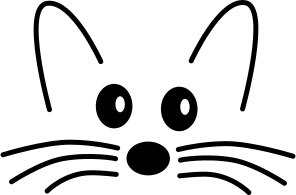
\includegraphics[width=1.4em]{squeak-logo}}}
\newcommand{\dothis}[1]{%
	\medskip
	\noindent\dothisicon
	\ifx#1\empty\else\quad\emph{#1}\fi
	\par\smallskip\nopagebreak}
% NB: To use this in an individual chapter, you must set:
%\graphicspath{{figures/} {../figures/}}
% at the head of the chapter.  Don't forget the final /
%=============================================================
%:Reader hints (hint)
%
% Indicates a non-obvious consequence 
\newcommand{\hint}[1]{\vspace{1ex}\noindent\fbox{\textsc{Astuce}} \emph{#1}}
%=================================================================
% graphics for Morphic handles
\newcommand{\grabHandle}{\raisebox{-0.2ex}{
\includegraphics[width=1em]{blackHandle}}}
\newcommand{\moveHandle}{\raisebox{-0.2ex}{
\includegraphics[width=1em]{moveHandle}}}
\newcommand{\debugHandle}{\raisebox{-0.2ex}{
\includegraphics[width=1em]{debugHandle}}}
% squeak-fr (added for Morphic handles)
\newcommand{\rotateHandle}{\raisebox{-0.2ex}{
\includegraphics[width=1em]{rotateHandle}}}
\newcommand{\viewerHandle}{\raisebox{-0.2ex}{
\includegraphics[width=1em]{viewerHandle}}}
% squeak-fr (add cloverHandle to use \clover in QuickTour.tex as alias
% todo 

%=============================================================
%:Highlighting Important stuff (doublebox)
%
% From Seaside book ...
\newsavebox{\SavedText}
\newlength{\InnerBoxRule}\setlength{\InnerBoxRule}{.75\fboxrule}
\newlength{\OuterBoxRule}\setlength{\OuterBoxRule}{1.5\fboxrule}
\newlength{\BoxSeparation}\setlength{\BoxSeparation}{1.5\fboxrule}
\addtolength{\BoxSeparation}{.5pt}
\newlength{\SaveBoxSep}\setlength{\SaveBoxSep}{2\fboxsep}
%
\newenvironment{doublebox}{\begin{lrbox}{\SavedText}
    \begin{minipage}{.75\textwidth}}
    {\end{minipage}\end{lrbox}\begin{center}
    \setlength{\fboxsep}{\BoxSeparation}\setlength{\fboxrule}{\OuterBoxRule}
    \fbox{\setlength{\fboxsep}{\SaveBoxSep}\setlength{\fboxrule}{\InnerBoxRule}%
      \fbox{\usebox{\SavedText}}}
  \end{center}}
% Use this:
\newcommand{\important}[1]{\begin{doublebox}#1\end{doublebox}}
%=============================================================
%:Section depth
\setcounter{secnumdepth}{2}
%% for this to happen start the file with
%\ifx\wholebook\relax\else
%% $Author$ Martial
% $Date$ Wed Oct 10 13:34:55 CEST 2007
% $Revision$ source: SBE 12715 
% Last Changed Date: 2007-10-08 21:32:45 +0200 (Mon, 08 Oct 2007)
%=============================================================
% NB: documentclass must be set in main document.
% Allows book to be generated in multiple formats.
%=============================================================
%:Packages
\usepackage[french]{babel}
\usepackage[T1]{fontenc}  %%%%%% really important to get the code directly in the text!
\usepackage{lmodern}
%\usepackage[scaled=0.85]{bookmanx} % needs another scale factor if used with \renewcommand{\sfdefault}{cmbr}
\usepackage{palatino}
\usepackage[scaled=0.85]{helvet}
\usepackage{microtype}
\usepackage{graphicx}
\usepackage{theorem}
\usepackage[utf8]{inputenc}
% ON: pdfsync breaks the use of p{width} for tabular columns!
\ifdefined\usepdfsync\usepackage{pdfsync}\fi % Requires texlive 2007
%=============================================================
%:More packages
%Stef should check which ones are used!
%\usepackage{picinpar}
%\usepackage{layout}
%\usepackage{color}
%\usepackage{enum}
%\usepackage{a4wide}
% \usepackage{fancyhdr}
\usepackage{ifthen}
\usepackage{float}
\usepackage{longtable}
\usepackage{makeidx}
\usepackage[nottoc]{tocbibind}
\usepackage{multicol}
\usepackage{booktabs}	% book-style tables
\usepackage{topcapt}	% enables \topcaption
\usepackage{multirow}
\usepackage{tabularx}
%\usepackage[bottom]{footmisc}
\usepackage{xspace}
\usepackage{alltt}
\usepackage{amssymb,textcomp}
\usepackage[usenames,dvipsnames]{color}
%\usepackage{colortbl}
\usepackage[hang]{subfigure}\makeatletter\def\p@subfigure{\thefigure\,}\makeatother
\usepackage{rotating}
\usepackage{enumitem}	% apb: allows more control over tags in enumerations
\usepackage{verbatim}     % for comment environment
\usepackage{varioref}	% for page references that work
\labelformat{footnote}{\thechapter--#1} % to distinguish citations from jurabib
\usepackage{needspace}
\usepackage{isodateo} % enable \isodate
\usepackage[newparttoc]{titlesec}
\usepackage{titletoc}
\usepackage{eurosym}
\usepackage{wrapfig}

\usepackage[
	super,
	citefull=first,
	authorformat={allreversed,and},
	titleformat={commasep,italic}
]{jurabib} % citations as footnotes
\usepackage[
	colorlinks=true,
	linkcolor=black,
	urlcolor=black,
	citecolor=black
]{hyperref}   % should come last

%=============================================================
%:URL style
\makeatletter

\def\url@leostyle{%
  \@ifundefined{selectfont}{\def\UrlFont{\sf}}{\def\UrlFont{\sffamily}}}
% ajouter par Martial pour \traduit (met une dague dans les \doublebox
\def\thempfootnote{\fnsymbol{mpfootnote}}

\makeatother
% Now actually use the newly defined style.
\urlstyle{leo}
%=============================================================
%:Booleans
\newboolean{lulu}
\setboolean{lulu}{false}
\newcommand{\ifluluelse}[2]{\ifthenelse{\boolean{lulu}}{#1}{#2}}
%=============================================================
%:Names
\newcommand{\SUnit}{SUnit\xspace}
\newcommand{\sunit}{SUnit\xspace}
\newcommand{\xUnit}{$x$Unit\xspace}
\newcommand{\JUnit}{JUnit\xspace}
%\newcommand{\XP}{eXtreme Programming\xspace}
\newcommand{\st}{Smalltalk\xspace}
\newcommand{\Squeak}{Squeak\xspace}
\newcommand{\sq}{Squeak\xspace}
\newcommand{\sqmap}{SqueakMap\xspace}
\newcommand{\squeak}{Squeak\xspace}
%\newcommand{\sbe}{\url{scg.unibe.ch/SBE}\xspace}
%\newcommand{\sbe}{\url{squeakbyexample.org}\xspace}
\newcommand{\sbe}{\url{SqueakByExample.org}\xspace}
% squeak-fr: adresse de la version francaise
\newcommand{\spe}{\url{SqueakByExample.org}\xspace} % ?/FR
\newcommand{\sba}{\url{SquareBracketAssociates.org}\xspace}

% squeak-fr: ajout de la \squeakdev pour eviter les problemes de
% changements d'url rencontres dans la VO:
\newcommand{\squeakdev}{\url{www.squeaksource.com/ImageForDevelopers}\xspace} %ou
%\newcommand{\squeakdev}{\url{squeak.ofset.org/squeak-dev}\xspace}

%=============================================================
%:Editorial comment macros
\newcommand{\nnbb}[2]{
    \fbox{\bfseries\sffamily\scriptsize#1}
    {\sf\small$\blacktriangleright$\textit{#2}$\blacktriangleleft$}
   }
\newcommand{\ab}[1]{\nnbb{Andrew}{#1}}
\newcommand{\sd}[1]{\nnbb{St\'{e}f}{#1}}
\newcommand{\md}[1]{\nnbb{Marcus}{#1}}
\newcommand{\on}[1]{\nnbb{Oscar}{#1}}
\newcommand{\damien}[1]{\nnbb{Damien}{#1}}
\newcommand{\lr}[1]{\nnbb{Lukas}{#1}}
\newcommand{\orla}[1]{\nnbb{Orla}{#1}}
%\newcommand{\here}{\nnbb{CONTINUE}{HERE}}
\newcommand{\here}{\nnbb{CONTINUE}{ICI}}

%=============================================================
%:Abbreviation macros
\newcommand{\ie}{\emph{c-\`a-d.}\xspace}
\newcommand{\cad}{\emph{c-\`a-d.}\xspace}
%\newcommand{\eg}{\emph{e.g.},\xspace}
\newcommand{\eg}{\emph{par ex.},\xspace}
\newcommand{\parex}{\emph{par ex.},\xspace}
\newcommand{\etc}{etc\xspace}
%=============================================================
%:Cross reference macros

% [squeak-fr] martial: remarquez les articles devant les noms
\newcommand{\charef}[1]{le chapitre~\ref{cha:#1}\xspace}
% note de martial: utilise dans chapitre Syntax.tex: a redefinir
\newcommand{\charefs}[2]{les chapitres~\ref{cha:#1} et \ref{cha:#2}\xspace}
\newcommand{\secref}[1]{la section~\ref{sec:#1}\xspace}
\newcommand{\figref}[1]{la figure~\ref{fig:#1}\xspace}
\newcommand{\Figref}[1]{La figure~\ref{fig:#1}\xspace}
\newcommand{\appref}[1]{l'annexe~\ref{app:#1}\xspace}
\newcommand{\tabref}[1]{la table~\ref{tab:#1}\xspace}
% defini pour le chapitre Messages.tex
\newcommand{\Tabref}[1]{La table~\ref{tab:#1}\xspace}

% APB: I removed trailing \xspace commands from these macros because
% \xspace mostly doesn't work.  If you want a space after your
% references, type one!
% ON: xspace has always worked just fine for me!  Please leave them in.
%
\newcommand{\ruleref}[1]{\ref{rule:#1}\xspace}
%
\newcommand{\egref}[1]{exemple~\ref{eg:#1}\xspace}
\newcommand{\Egref}[1]{Exemple~\ref{eg:#1}\xspace}
%
\newcommand{\scrref}[1]{script~\ref{scr:#1}\xspace}
\newcommand{\Scrref}[1]{Script~\ref{scr:#1}\xspace}
% t = the
\newcommand{\tscrref}[1]{le script~\ref{scr:#1}\xspace}
\newcommand{\Tscrref}[1]{Le script~\ref{scr:#1}\xspace}
%
\newcommand{\mthref}[1]{m\'ethode~\ref{mth:#1}\xspace}
\newcommand{\mthsref}[1]{m\'ethodes~\ref{mth:#1}\xspace}
\newcommand{\Mthref}[1]{M\'ethode~\ref{mth:#1}\xspace}
\newcommand{\tmthref}[1]{la m\'ethode~\ref{mth:#1}\xspace}
\newcommand{\Tmthref}[1]{La m\'ethode~\ref{mth:#1}\xspace}
%
\newcommand{\clsref}[1]{classe~\ref{cls:#1}\xspace}
\newcommand{\tclsref}[1]{la classe~\ref{cls:#1}\xspace}
\newcommand{\Tclsref}[1]{La classe~\ref{cls:#1}\xspace}
%=============================================================
%:Menu item macro
% for menu items, so we can change our minds on how to print them! (apb)
\definecolor{lightgray}{gray}{0.89}
\newcommand{\menu}[1]{{%
	\setlength{\fboxsep}{0pt}%
	\colorbox{lightgray}{{{\upshape\sffamily\strut \,#1\,}}}}}
% \newcommand{\menu}[1]{{%
% 	\fontfamily{lmr}\selectfont
% 	\upshape\textlangle{\sffamily #1}\textrangle}}
% For submenu items:
\newcommand{\go}{\,$\triangleright$\,}
% \newcommand{\go}{\,$\blacktriangleright$\,}
% For keyboard shortcuts:
%\newcommand{\short}[1]{\mbox{$\langle${\sc CMD}$\rangle$-#1}\xspace}
\newcommand{\short}[1]{\mbox{{\sc cmd}\hspace{0.08em}--\hspace{0.09em}#1}\xspace}
% For buttons:
\newcommand{\button}[1]{{%
	\setlength{\fboxsep}{0pt}%
	\fbox{{\upshape\sffamily\strut \,#1\,}}}}
\newcommand{\toolsflap}{l'onglet \textit{Tools}\xspace}
%=============================================================
%:Reader cues (do this)
%
% Indicate something the reader should try out.
\newcommand{\dothisicon}{\raisebox{-.5ex}{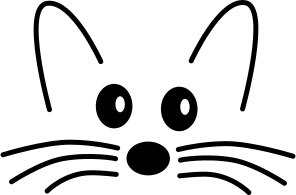
\includegraphics[width=1.4em]{squeak-logo}}}
\newcommand{\dothis}[1]{%
	\medskip
	\noindent\dothisicon
	\ifx#1\empty\else\quad\emph{#1}\fi
	\par\smallskip\nopagebreak}
% NB: To use this in an individual chapter, you must set:
%\graphicspath{{figures/} {../figures/}}
% at the head of the chapter.  Don't forget the final /
%=============================================================
%:Reader hints (hint)
%
% Indicates a non-obvious consequence 
\newcommand{\hint}[1]{\vspace{1ex}\noindent\fbox{\textsc{Astuce}} \emph{#1}}
%=================================================================
% graphics for Morphic handles
\newcommand{\grabHandle}{\raisebox{-0.2ex}{
\includegraphics[width=1em]{blackHandle}}}
\newcommand{\moveHandle}{\raisebox{-0.2ex}{
\includegraphics[width=1em]{moveHandle}}}
\newcommand{\debugHandle}{\raisebox{-0.2ex}{
\includegraphics[width=1em]{debugHandle}}}
% squeak-fr (added for Morphic handles)
\newcommand{\rotateHandle}{\raisebox{-0.2ex}{
\includegraphics[width=1em]{rotateHandle}}}
\newcommand{\viewerHandle}{\raisebox{-0.2ex}{
\includegraphics[width=1em]{viewerHandle}}}
% squeak-fr (add cloverHandle to use \clover in QuickTour.tex as alias
% todo 

%=============================================================
%:Highlighting Important stuff (doublebox)
%
% From Seaside book ...
\newsavebox{\SavedText}
\newlength{\InnerBoxRule}\setlength{\InnerBoxRule}{.75\fboxrule}
\newlength{\OuterBoxRule}\setlength{\OuterBoxRule}{1.5\fboxrule}
\newlength{\BoxSeparation}\setlength{\BoxSeparation}{1.5\fboxrule}
\addtolength{\BoxSeparation}{.5pt}
\newlength{\SaveBoxSep}\setlength{\SaveBoxSep}{2\fboxsep}
%
\newenvironment{doublebox}{\begin{lrbox}{\SavedText}
    \begin{minipage}{.75\textwidth}}
    {\end{minipage}\end{lrbox}\begin{center}
    \setlength{\fboxsep}{\BoxSeparation}\setlength{\fboxrule}{\OuterBoxRule}
    \fbox{\setlength{\fboxsep}{\SaveBoxSep}\setlength{\fboxrule}{\InnerBoxRule}%
      \fbox{\usebox{\SavedText}}}
  \end{center}}
% Use this:
\newcommand{\important}[1]{\begin{doublebox}#1\end{doublebox}}
%=============================================================
%:Section depth
\setcounter{secnumdepth}{2}
%% for this to happen start the file with
%\ifx\wholebook\relax\else
%% $Author$ Martial
% $Date$ Wed Oct 10 13:34:55 CEST 2007
% $Revision$ source: SBE 12715 
% Last Changed Date: 2007-10-08 21:32:45 +0200 (Mon, 08 Oct 2007)
%=============================================================
% NB: documentclass must be set in main document.
% Allows book to be generated in multiple formats.
%=============================================================
%:Packages
\usepackage[french]{babel}
\usepackage[T1]{fontenc}  %%%%%% really important to get the code directly in the text!
\usepackage{lmodern}
%\usepackage[scaled=0.85]{bookmanx} % needs another scale factor if used with \renewcommand{\sfdefault}{cmbr}
\usepackage{palatino}
\usepackage[scaled=0.85]{helvet}
\usepackage{microtype}
\usepackage{graphicx}
\usepackage{theorem}
\usepackage[utf8]{inputenc}
% ON: pdfsync breaks the use of p{width} for tabular columns!
\ifdefined\usepdfsync\usepackage{pdfsync}\fi % Requires texlive 2007
%=============================================================
%:More packages
%Stef should check which ones are used!
%\usepackage{picinpar}
%\usepackage{layout}
%\usepackage{color}
%\usepackage{enum}
%\usepackage{a4wide}
% \usepackage{fancyhdr}
\usepackage{ifthen}
\usepackage{float}
\usepackage{longtable}
\usepackage{makeidx}
\usepackage[nottoc]{tocbibind}
\usepackage{multicol}
\usepackage{booktabs}	% book-style tables
\usepackage{topcapt}	% enables \topcaption
\usepackage{multirow}
\usepackage{tabularx}
%\usepackage[bottom]{footmisc}
\usepackage{xspace}
\usepackage{alltt}
\usepackage{amssymb,textcomp}
\usepackage[usenames,dvipsnames]{color}
%\usepackage{colortbl}
\usepackage[hang]{subfigure}\makeatletter\def\p@subfigure{\thefigure\,}\makeatother
\usepackage{rotating}
\usepackage{enumitem}	% apb: allows more control over tags in enumerations
\usepackage{verbatim}     % for comment environment
\usepackage{varioref}	% for page references that work
\labelformat{footnote}{\thechapter--#1} % to distinguish citations from jurabib
\usepackage{needspace}
\usepackage{isodateo} % enable \isodate
\usepackage[newparttoc]{titlesec}
\usepackage{titletoc}
\usepackage{eurosym}
\usepackage{wrapfig}

\usepackage[
	super,
	citefull=first,
	authorformat={allreversed,and},
	titleformat={commasep,italic}
]{jurabib} % citations as footnotes
\usepackage[
	colorlinks=true,
	linkcolor=black,
	urlcolor=black,
	citecolor=black
]{hyperref}   % should come last

%=============================================================
%:URL style
\makeatletter

\def\url@leostyle{%
  \@ifundefined{selectfont}{\def\UrlFont{\sf}}{\def\UrlFont{\sffamily}}}
% ajouter par Martial pour \traduit (met une dague dans les \doublebox
\def\thempfootnote{\fnsymbol{mpfootnote}}

\makeatother
% Now actually use the newly defined style.
\urlstyle{leo}
%=============================================================
%:Booleans
\newboolean{lulu}
\setboolean{lulu}{false}
\newcommand{\ifluluelse}[2]{\ifthenelse{\boolean{lulu}}{#1}{#2}}
%=============================================================
%:Names
\newcommand{\SUnit}{SUnit\xspace}
\newcommand{\sunit}{SUnit\xspace}
\newcommand{\xUnit}{$x$Unit\xspace}
\newcommand{\JUnit}{JUnit\xspace}
%\newcommand{\XP}{eXtreme Programming\xspace}
\newcommand{\st}{Smalltalk\xspace}
\newcommand{\Squeak}{Squeak\xspace}
\newcommand{\sq}{Squeak\xspace}
\newcommand{\sqmap}{SqueakMap\xspace}
\newcommand{\squeak}{Squeak\xspace}
%\newcommand{\sbe}{\url{scg.unibe.ch/SBE}\xspace}
%\newcommand{\sbe}{\url{squeakbyexample.org}\xspace}
\newcommand{\sbe}{\url{SqueakByExample.org}\xspace}
% squeak-fr: adresse de la version francaise
\newcommand{\spe}{\url{SqueakByExample.org}\xspace} % ?/FR
\newcommand{\sba}{\url{SquareBracketAssociates.org}\xspace}

% squeak-fr: ajout de la \squeakdev pour eviter les problemes de
% changements d'url rencontres dans la VO:
\newcommand{\squeakdev}{\url{www.squeaksource.com/ImageForDevelopers}\xspace} %ou
%\newcommand{\squeakdev}{\url{squeak.ofset.org/squeak-dev}\xspace}

%=============================================================
%:Editorial comment macros
\newcommand{\nnbb}[2]{
    \fbox{\bfseries\sffamily\scriptsize#1}
    {\sf\small$\blacktriangleright$\textit{#2}$\blacktriangleleft$}
   }
\newcommand{\ab}[1]{\nnbb{Andrew}{#1}}
\newcommand{\sd}[1]{\nnbb{St\'{e}f}{#1}}
\newcommand{\md}[1]{\nnbb{Marcus}{#1}}
\newcommand{\on}[1]{\nnbb{Oscar}{#1}}
\newcommand{\damien}[1]{\nnbb{Damien}{#1}}
\newcommand{\lr}[1]{\nnbb{Lukas}{#1}}
\newcommand{\orla}[1]{\nnbb{Orla}{#1}}
%\newcommand{\here}{\nnbb{CONTINUE}{HERE}}
\newcommand{\here}{\nnbb{CONTINUE}{ICI}}

%=============================================================
%:Abbreviation macros
\newcommand{\ie}{\emph{c-\`a-d.}\xspace}
\newcommand{\cad}{\emph{c-\`a-d.}\xspace}
%\newcommand{\eg}{\emph{e.g.},\xspace}
\newcommand{\eg}{\emph{par ex.},\xspace}
\newcommand{\parex}{\emph{par ex.},\xspace}
\newcommand{\etc}{etc\xspace}
%=============================================================
%:Cross reference macros

% [squeak-fr] martial: remarquez les articles devant les noms
\newcommand{\charef}[1]{le chapitre~\ref{cha:#1}\xspace}
% note de martial: utilise dans chapitre Syntax.tex: a redefinir
\newcommand{\charefs}[2]{les chapitres~\ref{cha:#1} et \ref{cha:#2}\xspace}
\newcommand{\secref}[1]{la section~\ref{sec:#1}\xspace}
\newcommand{\figref}[1]{la figure~\ref{fig:#1}\xspace}
\newcommand{\Figref}[1]{La figure~\ref{fig:#1}\xspace}
\newcommand{\appref}[1]{l'annexe~\ref{app:#1}\xspace}
\newcommand{\tabref}[1]{la table~\ref{tab:#1}\xspace}
% defini pour le chapitre Messages.tex
\newcommand{\Tabref}[1]{La table~\ref{tab:#1}\xspace}

% APB: I removed trailing \xspace commands from these macros because
% \xspace mostly doesn't work.  If you want a space after your
% references, type one!
% ON: xspace has always worked just fine for me!  Please leave them in.
%
\newcommand{\ruleref}[1]{\ref{rule:#1}\xspace}
%
\newcommand{\egref}[1]{exemple~\ref{eg:#1}\xspace}
\newcommand{\Egref}[1]{Exemple~\ref{eg:#1}\xspace}
%
\newcommand{\scrref}[1]{script~\ref{scr:#1}\xspace}
\newcommand{\Scrref}[1]{Script~\ref{scr:#1}\xspace}
% t = the
\newcommand{\tscrref}[1]{le script~\ref{scr:#1}\xspace}
\newcommand{\Tscrref}[1]{Le script~\ref{scr:#1}\xspace}
%
\newcommand{\mthref}[1]{m\'ethode~\ref{mth:#1}\xspace}
\newcommand{\mthsref}[1]{m\'ethodes~\ref{mth:#1}\xspace}
\newcommand{\Mthref}[1]{M\'ethode~\ref{mth:#1}\xspace}
\newcommand{\tmthref}[1]{la m\'ethode~\ref{mth:#1}\xspace}
\newcommand{\Tmthref}[1]{La m\'ethode~\ref{mth:#1}\xspace}
%
\newcommand{\clsref}[1]{classe~\ref{cls:#1}\xspace}
\newcommand{\tclsref}[1]{la classe~\ref{cls:#1}\xspace}
\newcommand{\Tclsref}[1]{La classe~\ref{cls:#1}\xspace}
%=============================================================
%:Menu item macro
% for menu items, so we can change our minds on how to print them! (apb)
\definecolor{lightgray}{gray}{0.89}
\newcommand{\menu}[1]{{%
	\setlength{\fboxsep}{0pt}%
	\colorbox{lightgray}{{{\upshape\sffamily\strut \,#1\,}}}}}
% \newcommand{\menu}[1]{{%
% 	\fontfamily{lmr}\selectfont
% 	\upshape\textlangle{\sffamily #1}\textrangle}}
% For submenu items:
\newcommand{\go}{\,$\triangleright$\,}
% \newcommand{\go}{\,$\blacktriangleright$\,}
% For keyboard shortcuts:
%\newcommand{\short}[1]{\mbox{$\langle${\sc CMD}$\rangle$-#1}\xspace}
\newcommand{\short}[1]{\mbox{{\sc cmd}\hspace{0.08em}--\hspace{0.09em}#1}\xspace}
% For buttons:
\newcommand{\button}[1]{{%
	\setlength{\fboxsep}{0pt}%
	\fbox{{\upshape\sffamily\strut \,#1\,}}}}
\newcommand{\toolsflap}{l'onglet \textit{Tools}\xspace}
%=============================================================
%:Reader cues (do this)
%
% Indicate something the reader should try out.
\newcommand{\dothisicon}{\raisebox{-.5ex}{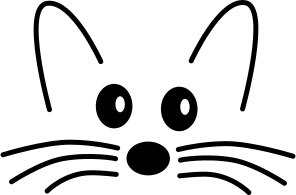
\includegraphics[width=1.4em]{squeak-logo}}}
\newcommand{\dothis}[1]{%
	\medskip
	\noindent\dothisicon
	\ifx#1\empty\else\quad\emph{#1}\fi
	\par\smallskip\nopagebreak}
% NB: To use this in an individual chapter, you must set:
%\graphicspath{{figures/} {../figures/}}
% at the head of the chapter.  Don't forget the final /
%=============================================================
%:Reader hints (hint)
%
% Indicates a non-obvious consequence 
\newcommand{\hint}[1]{\vspace{1ex}\noindent\fbox{\textsc{Astuce}} \emph{#1}}
%=================================================================
% graphics for Morphic handles
\newcommand{\grabHandle}{\raisebox{-0.2ex}{
\includegraphics[width=1em]{blackHandle}}}
\newcommand{\moveHandle}{\raisebox{-0.2ex}{
\includegraphics[width=1em]{moveHandle}}}
\newcommand{\debugHandle}{\raisebox{-0.2ex}{
\includegraphics[width=1em]{debugHandle}}}
% squeak-fr (added for Morphic handles)
\newcommand{\rotateHandle}{\raisebox{-0.2ex}{
\includegraphics[width=1em]{rotateHandle}}}
\newcommand{\viewerHandle}{\raisebox{-0.2ex}{
\includegraphics[width=1em]{viewerHandle}}}
% squeak-fr (add cloverHandle to use \clover in QuickTour.tex as alias
% todo 

%=============================================================
%:Highlighting Important stuff (doublebox)
%
% From Seaside book ...
\newsavebox{\SavedText}
\newlength{\InnerBoxRule}\setlength{\InnerBoxRule}{.75\fboxrule}
\newlength{\OuterBoxRule}\setlength{\OuterBoxRule}{1.5\fboxrule}
\newlength{\BoxSeparation}\setlength{\BoxSeparation}{1.5\fboxrule}
\addtolength{\BoxSeparation}{.5pt}
\newlength{\SaveBoxSep}\setlength{\SaveBoxSep}{2\fboxsep}
%
\newenvironment{doublebox}{\begin{lrbox}{\SavedText}
    \begin{minipage}{.75\textwidth}}
    {\end{minipage}\end{lrbox}\begin{center}
    \setlength{\fboxsep}{\BoxSeparation}\setlength{\fboxrule}{\OuterBoxRule}
    \fbox{\setlength{\fboxsep}{\SaveBoxSep}\setlength{\fboxrule}{\InnerBoxRule}%
      \fbox{\usebox{\SavedText}}}
  \end{center}}
% Use this:
\newcommand{\important}[1]{\begin{doublebox}#1\end{doublebox}}
%=============================================================
%:Section depth
\setcounter{secnumdepth}{2}
%% for this to happen start the file with
%\ifx\wholebook\relax\else
%\input{../common.tex}
%\begin{document}
%\fi
% and terminate by
% \ifx\wholebook\relax\else\end{document}\fi

\DeclareGraphicsExtensions{.pdf, .jpg, .png}
%=============================================================
%:PDF setup
\hypersetup{
%   a4paper,
%   pdfstartview=FitV,
%   colorlinks,
%   linkcolor=darkblue,
%   citecolor=darkblue,
%   pdftitle={Squeak by Example},
pdftitle={Squeak par l'exemple},
   pdfauthor={Andrew Black, St\'ephane Ducasse,	Oscar Nierstrasz,
Damien Pollet},
   pdfkeywords={Smalltalk, Squeak, Programmation Orient\'ee Objet},
pdfsubject={Informatique, Computer Science}
}
%=============================================================
%:Page layout and appearance
%
% \renewcommand{\headrulewidth}{0pt}
\renewcommand{\chaptermark}[1]{\markboth{#1}{}}
\renewcommand{\sectionmark}[1]{\markright{\thesection\ #1}}
\renewpagestyle{plain}[\small\itshape]{%
	\setheadrule{0pt}%
	\sethead[\thepage][][]{}{}{\thepage}%
	\setfoot[][][]{}{}{}}
\renewpagestyle{headings}[\small\itshape]{%
	\setheadrule{0pt}%
	\setmarks{chapter}{section}%
	\sethead[\thepage][][\chaptertitle]{\sectiontitle}{}{\thepage}%
	\setfoot[][][]{}{}{}}
%=============================================================
%:Title section setup and TOC numbering depth
\setcounter{secnumdepth}{1}
\setcounter{tocdepth}{1}
\titleformat{\part}[display]{\centering}{\huge\partname\ \thepart}{1em}{\Huge\textbf}[]
\titleformat{\chapter}[display]{}{\huge\chaptertitlename\ \thechapter}{1em}{\Huge\raggedright\textbf}[]
\titlecontents{part}[3pc]{%
		\pagebreak[2]\addvspace{1em plus.4em minus.2em}%
		\leavevmode\large\bfseries}
	{\contentslabel{3pc}}{\hspace*{-3pc}}
	{}[\nopagebreak]
\titlecontents{chapter}[3pc]{%
		\pagebreak[0]\addvspace{1em plus.2em minus.2em}%
		\leavevmode\bfseries}
	{\contentslabel{3pc}}{}
	{\hfill\contentspage}[\nopagebreak]
\dottedcontents{section}[3pc]{}{3pc}{1pc}
\dottedcontents{subsection}[3pc]{}{0pc}{1pc}
% \dottedcontents{subsection}[4.5em]{}{0pt}{1pc}
% Make \cleardoublepage insert really blank pages http://www.tex.ac.uk/cgi-bin/texfaq2html?label=reallyblank
\let\origdoublepage\cleardoublepage
\newcommand{\clearemptydoublepage}{%
  \clearpage
  {\pagestyle{empty}\origdoublepage}}
\let\cleardoublepage\clearemptydoublepage % see http://www.tex.ac.uk/cgi-bin/texfaq2html?label=patch
%=============================================================
%:FAQ macros (for FAQ chapter)
\newtheorem{faq}{FAQ}
\newcommand{\answer}{\paragraph{R\'eponse}\ }
%=============================================================
%:Listings package configuration
\usepackage{listings}
\newcommand{\caret}{\makebox{\raisebox{0.4ex}{\footnotesize{$\wedge$}}}}
\lstdefinelanguage{Smalltalk}{
%  morekeywords={self,super,true,false,nil,thisContext}, % This is overkill
  morestring=[d]',
  morecomment=[s]{"}{"},
  alsoletter={\#:},
  escapechar={!},
  escapebegin=\itshape, % comment-like by default (Martial 11/2007)
  literate=
    {BANG}{!}1
    {UNDERSCORE}{\_}1
    {\\st}{Smalltalk}9 % convenience -- in case \st occurs in code
    % {'}{{\textquotesingle}}1 % replaced by upquote=true in \lstset
    {_}{{$\leftarrow$}}1
    {>>>}{{\sep}}1
    {^}{{$\uparrow$}}1
    {~}{{$\sim$}}1
    {-}{{\sf -\hspace{-0.13em}-}}1  % the goal is to make - the same width as +
    {+}{\raisebox{0.08ex}{+}}1		% and to raise + off the baseline to match -
    {-->}{{\quad$\longrightarrow$\quad}}3
	, % Don't forget the comma at the end!
  tabsize=4
}[keywords,comments,strings]
% ajout pour les échappements dans les codes
% indispensable pour mettre le code en emphase (cf. Model.tex) 
\newcommand{\codeify}[1]{\NoAutoSpaceBeforeFDP#1\AutoSpaceBeforeFDP}
\newcommand{\normcomment}[1]{\emph{#1}} %cf. Streams
\newcommand{\normcode}[1]{\emph{\codeify{#1}}} %cf. Streams
\newcommand{\emcode}[1]{\textbf{\normcode{#1}}} % Martial 11/2007
\lstset{language=Smalltalk,
	basicstyle=\sffamily,
	keywordstyle=\color{black}\bfseries,
	% stringstyle=\ttfamily, % Ugly! do we really want this? -- on
	%commentstyle=\itshape,
	mathescape=true,
	showstringspaces=false,
	keepspaces=true,
	breaklines=true,
	breakautoindent=true,
	lineskip={-1pt}, % Ugly hack
	upquote=true, % straight quote; requires textcomp package
	columns=fullflexible} % no fixed width fonts
% In-line code (literal)
% Normally use this for all in-line code:
\newcommand{\ct}{\lstinline[mathescape=false,basicstyle={\sffamily\upshape}]}
% apb 2007.8.28 added the \upshape declaration to avoid getting italicized code in \dothis{ } sections.
% In-line code (latex enabled)
% Use this only in special situations where \ct does not work
% (within section headings ...):

% [squeak-fr] Modification de \lct suivant les indications de Martial Boniou
\newcommand{\lct}[1]{\textsf{\textup{\NoAutoSpaceBeforeFDP #1
\AutoSpaceBeforeFDP}}} %\xspace

% Use these for system categories and protocols:
\newcommand{\scat}[1]{\emph{\textsf{#1}}\xspace}
\newcommand{\pkg}[1]{\emph{\textsf{#1}}\xspace}
\newcommand{\prot}[1]{\emph{\textsf{#1}}\xspace}
% Code environments
% NB: the arg is for tests
% Only code and example environments may be tests
\lstnewenvironment{code}[1]{%
	\lstset{%
		frame=lines,
		mathescape=false
	}
}{}
\def\ignoredollar#1{}
%=============================================================
%:Code environments (method, script ...)
% NB: the third arg is for tests
% Only code and example environments may be tests
\lstnewenvironment{example}[3][defaultlabel]{%
	\renewcommand{\lstlistingname}{Exemple}%
	\lstset{
		frame=lines,
		mathescape=false,
		caption={\emph{#2}},
		label={eg:#1}
	}
}{}
\lstnewenvironment{script}[2][defaultlabel]{%
\renewcommand{\lstlistingname}{Script}%
	\lstset{
		frame=lines,
		mathescape=false,
		name={Script},
		caption={\emph{#2}},
		label={scr:#1}
	}
}{}
\lstnewenvironment{method}[2][defaultlabel]{%
	\renewcommand{\lstlistingname}{M\'ethode}%
	\lstset{
		frame=lines,
		mathescape=false,
		name={M\'ethode},
		caption={\emph{#2}},
		label={mth:#1}
	}
}{}
\lstnewenvironment{methods}[2][defaultlabel]{% just for multiple methods at once
	\renewcommand{\lstlistingname}{M\'ethodes}%
	\lstset{
		frame=lines,
		mathescape=false,
		name={M\'ethode},
		caption={\emph{#2}},
		label={mth:#1}
	}
}{}
\lstnewenvironment{numMethod}[2][defaultlabel]{%
	\renewcommand{\lstlistingname}{M\'ethode}%
	\lstset{
		numbers=left,
		numberstyle={\tiny\sffamily},
		frame=lines,
		mathescape=false,
		name={M\'ethode},
		caption={\emph{#2}},
		label={mth:#1}
	}
}{}
\lstnewenvironment{classdef}[2][defaultlabel]{%
	\renewcommand{\lstlistingname}{Classe}%
	\lstset{
		frame=lines,
		mathescape=false,
		name={Classe},
		caption={\emph{#2}},
		label={cls:#1}
	}
}{}
%=============================================================
%:Reserving space
% Usually need one more line than the actual lines of code
\newcommand{\needlines}[1]{\Needspace{#1\baselineskip}}
%=============================================================
%:Indexing macros
% Macros ending with "ind" generate text as well as an index entry
% Macros ending with "index" *only* generate an index entry
\newcommand{\ind}[1]{\index{#1}#1\xspace} % plain text
\newcommand{\subind}[2]{\index{#1!#2}#2\xspace} % show #2, subindex inder #1
\newcommand{\emphind}[1]{\index{#1}\emph{#1}\xspace} % emph #1
\newcommand{\emphsubind}[2]{\index{#1!#2}\emph{#2}\xspace} % show emph #2, subindex inder #1
\newcommand{\scatind}[1]{\index{#1@\textsf{#1} (cat\'egorie)}\scat{#1}} % category
\newcommand{\protind}[1]{\index{#1@\textsf{#1} (protocole)}\prot{#1}} % protocol
% \newcommand{\clsind}[1]{\index{#1@\textsf{#1} (class)}\ct{#1}\xspace}
\newcommand{\clsind}[1]{\index{#1!\#@(classe)}\ct{#1}\xspace} % class
\newcommand{\cvind}[1]{\index{#1@\textsf{#1} (variable de classe)}\ct{#1}\xspace} % class var
\newcommand{\glbind}[1]{\index{#1@\textsf{#1} (globale)}\ct{#1}\xspace} % global
\newcommand{\patind}[1]{\index{#1@#1 (patron)}\ct{#1}\xspace} % pattern
\newcommand{\pvind}[1]{\index{#1@\textsf{#1} (pseudo-variable)}\ct{#1}\xspace} % pseudo variable
% [squeak - fr]Martial: I found the following cleaner (should be
% merged in SBE for self and super)
\newcommand{\subpvindex}[2]{\index{#1@\textsf{#1} (pseudo-variable)!#2}}
\newcommand{\subpvind}[2]{\index{#1@\textsf{#1} (pseudo-variable)!#2}#2\xspace}
% used in Model.tex
\newcommand{\mthind}[2]{\index{#1!#2@\ct{#2}}\ct{#2}\xspace} % show method name only
\newcommand{\lmthind}[2]{\index{#1!#2@\ct{#2}}\lct{#2}\xspace} % show method name only
\newcommand{\cmind}[2]{\index{#1!#2@\ct{#2}}\ct{#1>>>#2}\xspace} % show class>>method
\newcommand{\toolsflapind}{\index{onglet Tools}\toolsflap} % index tools flap
% The following only generate an index entry:
% \newcommand{\clsindex}[1]{\index{#1@\textsf{#1} (class)}}
\newcommand{\clsindex}[1]{\index{#1!\#@(classe)}} % class
\newcommand{\cmindex}[2]{\index{#1!#2@\ct{#2}}} % class>>method
\newcommand{\cvindex}[1]{\index{#1@\textsf{#1} (variable de classe)}} % class var
\newcommand{\glbindex}[1]{\index{#1@\textsf{#1} (globale)}}% global
\newcommand{\pvindex}[1]{\index{#1@\textsf{#1} (pseudo-variable)}}% pseudo var
\newcommand{\seeindex}[2]{\index{#1|see{#2}}} % #1, see #2
\newcommand{\scatindex}[1]{\index{#1@\textsf{#1} (cat\'egorie)}} % category
\newcommand{\protindex}[1]{\index{#1@\textsf{#1} (protocole)}} % protocol
% How can we have the main entry page numbers in bold yet not break the hyperlink?
\newcommand{\boldidx}[1]{{\bf #1}} % breaks hyperlink
%\newcommand{\indmain}[1]{\index{#1|boldidx}#1\xspace} % plain text, main entry
%\newcommand{\emphsubindmain}[2]{\index{#1!#2|boldidx}\emph{#2}\xspace} % subindex, main entry
%\newcommand{\subindmain}[2]{\index{#1!#2|boldidx}#2\xspace} % subindex, main entry
%\newcommand{\clsindmain}[1]{\index{#1@\textsf{#1} (class)|boldidx}\ct{#1}\xspace}
%\newcommand{\clsindmain}[1]{\index{#1!\#@(class)|boldidx}\ct{#1}\xspace} % class main
%\newcommand{\indexmain}[1]{\index{#1|boldidx}} % main index entry only
\newcommand{\indmain}[1]{\index{#1}#1\xspace} 
\newcommand{\emphsubindmain}[2]{\index{#1!#2}\emph{#2}\xspace} % subindex, main entry
\newcommand{\subindmain}[2]{\index{#1!#2}#2\xspace} % subindex, main entry
%\newcommand{\clsindmain}[1]{\index{#1@\textsf{#1} (class)}\ct{#1}\xspace}
\newcommand{\clsindmain}[1]{\index{#1!\#@(classe)}\ct{#1}\xspace} % class main
\newcommand{\indexmain}[1]{\index{#1}} 
%=============================================================
%:Code macros
% some constants
\newcommand{\codesize}{\small}
\newcommand{\codefont}{\sffamily}
\newcommand{\cat}[1]{\textit{Dans la cat\'egorie #1}}%%To remove later
\newlength{\scriptindent}
\setlength{\scriptindent}{.3cm}
%% Method presentation constants
\newlength{\methodindent}
\newlength{\methodwordlength}
\newlength{\aftermethod}
\setlength{\methodindent}{0.2cm}
\settowidth{\methodwordlength}{\ M\'ethode\ }
%=============================================================
%:Smalltalk macros
%\newcommand{\sep}{{$\gg$}}
\newcommand{\sep}{\mbox{>>}}
\newcommand{\self}{\ct{self}\xspace}
\newcommand{\super}{\ct{super}\xspace}
\newcommand{\nil}{\ct{nil}\xspace}
%=============================================================
% be less conservative about float placement
% these commands are from http://www.tex.ac.uk/cgi-bin/texfaq2html?label=floats
\renewcommand{\topfraction}{.9}
\renewcommand{\bottomfraction}{.9}
\renewcommand{\textfraction}{.1}
\renewcommand{\floatpagefraction}{.85}
\renewcommand{\dbltopfraction}{.66}
\renewcommand{\dblfloatpagefraction}{.85}
\setcounter{topnumber}{9}
\setcounter{bottomnumber}{9}
\setcounter{totalnumber}{20}
\setcounter{dbltopnumber}{9}
%=============================================================
%% [Squeak-fr]
% pour identifier les zones de texte à corriger d'urgence!
\newcommand{\arevoir}[1]{#1}
% \traduit utilisé dans Model.tex
\newcommand{\traduit}[1]{\footnote[2]{#1}}
% changeset alias
\newcommand{\changeset}{\emph{change set}\xspace}
\newcommand{\changesets}{\emph{change sets}\xspace}
% callback alias
\newcommand{\callback}{\emph{callback}\xspace}
% blobmorph alias (QuickTour->blob)
\newcommand{\blobmorph}{\emph{blob}\xspace}
% repository
\newcommand{\squeaksource}{\textsf{SqueakSource}\xspace}
\newcommand{\sourceforge}{\textsf{SourceForge}\xspace}
% L'onglet Tools
\newcommand{\Toolsflap}{L'onglet \textit{Tools}\xspace}
% Mac OS X
\newcommand{\macosx}{\mbox{Mac OS X}\xspace}
% code en francais (uniquement dans le chapitre BasicClasses)
\newcommand{\codefrench}[1]{\NoAutoSpaceBeforeFDP\texttt{#1}\AutoSpaceBeforeFDP\xspace}
% mantra du modele objet (suite a l'erreur de martial)
\newcommand{\Mantra}{Tout est objet\xspace}
\newcommand{\mantra}{\MakeLowercase{\Mantra}\xspace}
% césure
\hyphenation{Omni-Brow-ser}
\hyphenation{m\'e-tho-de} % erreur de cesure commune
\hyphenation{m\'e-tho-des}
\hyphenation{e-xem-ple}
\hyphenation{en-re-gi-stre}
\hyphenation{a-na-ly-seur}
\hyphenation{glo-ba-le}
\hyphenation{fi-gu-re}
\hyphenation{vi-si-bles}
\hyphenation{cor-res-pon-dan-te}
\hyphenation{Work-space}
%=============================================================
% apb doesn't like paragraphs to run in to each other without a break
\parskip 1ex
%=============================================================
%:Stuff to check, merge or deprecate
%\setlength{\marginparsep}{2mm}
%\renewcommand{\baselinestretch}{1.1}
%=============================================================

%\begin{document}
%\fi
% and terminate by
% \ifx\wholebook\relax\else\end{document}\fi

\DeclareGraphicsExtensions{.pdf, .jpg, .png}
%=============================================================
%:PDF setup
\hypersetup{
%   a4paper,
%   pdfstartview=FitV,
%   colorlinks,
%   linkcolor=darkblue,
%   citecolor=darkblue,
%   pdftitle={Squeak by Example},
pdftitle={Squeak par l'exemple},
   pdfauthor={Andrew Black, St\'ephane Ducasse,	Oscar Nierstrasz,
Damien Pollet},
   pdfkeywords={Smalltalk, Squeak, Programmation Orient\'ee Objet},
pdfsubject={Informatique, Computer Science}
}
%=============================================================
%:Page layout and appearance
%
% \renewcommand{\headrulewidth}{0pt}
\renewcommand{\chaptermark}[1]{\markboth{#1}{}}
\renewcommand{\sectionmark}[1]{\markright{\thesection\ #1}}
\renewpagestyle{plain}[\small\itshape]{%
	\setheadrule{0pt}%
	\sethead[\thepage][][]{}{}{\thepage}%
	\setfoot[][][]{}{}{}}
\renewpagestyle{headings}[\small\itshape]{%
	\setheadrule{0pt}%
	\setmarks{chapter}{section}%
	\sethead[\thepage][][\chaptertitle]{\sectiontitle}{}{\thepage}%
	\setfoot[][][]{}{}{}}
%=============================================================
%:Title section setup and TOC numbering depth
\setcounter{secnumdepth}{1}
\setcounter{tocdepth}{1}
\titleformat{\part}[display]{\centering}{\huge\partname\ \thepart}{1em}{\Huge\textbf}[]
\titleformat{\chapter}[display]{}{\huge\chaptertitlename\ \thechapter}{1em}{\Huge\raggedright\textbf}[]
\titlecontents{part}[3pc]{%
		\pagebreak[2]\addvspace{1em plus.4em minus.2em}%
		\leavevmode\large\bfseries}
	{\contentslabel{3pc}}{\hspace*{-3pc}}
	{}[\nopagebreak]
\titlecontents{chapter}[3pc]{%
		\pagebreak[0]\addvspace{1em plus.2em minus.2em}%
		\leavevmode\bfseries}
	{\contentslabel{3pc}}{}
	{\hfill\contentspage}[\nopagebreak]
\dottedcontents{section}[3pc]{}{3pc}{1pc}
\dottedcontents{subsection}[3pc]{}{0pc}{1pc}
% \dottedcontents{subsection}[4.5em]{}{0pt}{1pc}
% Make \cleardoublepage insert really blank pages http://www.tex.ac.uk/cgi-bin/texfaq2html?label=reallyblank
\let\origdoublepage\cleardoublepage
\newcommand{\clearemptydoublepage}{%
  \clearpage
  {\pagestyle{empty}\origdoublepage}}
\let\cleardoublepage\clearemptydoublepage % see http://www.tex.ac.uk/cgi-bin/texfaq2html?label=patch
%=============================================================
%:FAQ macros (for FAQ chapter)
\newtheorem{faq}{FAQ}
\newcommand{\answer}{\paragraph{R\'eponse}\ }
%=============================================================
%:Listings package configuration
\usepackage{listings}
\newcommand{\caret}{\makebox{\raisebox{0.4ex}{\footnotesize{$\wedge$}}}}
\lstdefinelanguage{Smalltalk}{
%  morekeywords={self,super,true,false,nil,thisContext}, % This is overkill
  morestring=[d]',
  morecomment=[s]{"}{"},
  alsoletter={\#:},
  escapechar={!},
  escapebegin=\itshape, % comment-like by default (Martial 11/2007)
  literate=
    {BANG}{!}1
    {UNDERSCORE}{\_}1
    {\\st}{Smalltalk}9 % convenience -- in case \st occurs in code
    % {'}{{\textquotesingle}}1 % replaced by upquote=true in \lstset
    {_}{{$\leftarrow$}}1
    {>>>}{{\sep}}1
    {^}{{$\uparrow$}}1
    {~}{{$\sim$}}1
    {-}{{\sf -\hspace{-0.13em}-}}1  % the goal is to make - the same width as +
    {+}{\raisebox{0.08ex}{+}}1		% and to raise + off the baseline to match -
    {-->}{{\quad$\longrightarrow$\quad}}3
	, % Don't forget the comma at the end!
  tabsize=4
}[keywords,comments,strings]
% ajout pour les échappements dans les codes
% indispensable pour mettre le code en emphase (cf. Model.tex) 
\newcommand{\codeify}[1]{\NoAutoSpaceBeforeFDP#1\AutoSpaceBeforeFDP}
\newcommand{\normcomment}[1]{\emph{#1}} %cf. Streams
\newcommand{\normcode}[1]{\emph{\codeify{#1}}} %cf. Streams
\newcommand{\emcode}[1]{\textbf{\normcode{#1}}} % Martial 11/2007
\lstset{language=Smalltalk,
	basicstyle=\sffamily,
	keywordstyle=\color{black}\bfseries,
	% stringstyle=\ttfamily, % Ugly! do we really want this? -- on
	%commentstyle=\itshape,
	mathescape=true,
	showstringspaces=false,
	keepspaces=true,
	breaklines=true,
	breakautoindent=true,
	lineskip={-1pt}, % Ugly hack
	upquote=true, % straight quote; requires textcomp package
	columns=fullflexible} % no fixed width fonts
% In-line code (literal)
% Normally use this for all in-line code:
\newcommand{\ct}{\lstinline[mathescape=false,basicstyle={\sffamily\upshape}]}
% apb 2007.8.28 added the \upshape declaration to avoid getting italicized code in \dothis{ } sections.
% In-line code (latex enabled)
% Use this only in special situations where \ct does not work
% (within section headings ...):

% [squeak-fr] Modification de \lct suivant les indications de Martial Boniou
\newcommand{\lct}[1]{\textsf{\textup{\NoAutoSpaceBeforeFDP #1
\AutoSpaceBeforeFDP}}} %\xspace

% Use these for system categories and protocols:
\newcommand{\scat}[1]{\emph{\textsf{#1}}\xspace}
\newcommand{\pkg}[1]{\emph{\textsf{#1}}\xspace}
\newcommand{\prot}[1]{\emph{\textsf{#1}}\xspace}
% Code environments
% NB: the arg is for tests
% Only code and example environments may be tests
\lstnewenvironment{code}[1]{%
	\lstset{%
		frame=lines,
		mathescape=false
	}
}{}
\def\ignoredollar#1{}
%=============================================================
%:Code environments (method, script ...)
% NB: the third arg is for tests
% Only code and example environments may be tests
\lstnewenvironment{example}[3][defaultlabel]{%
	\renewcommand{\lstlistingname}{Exemple}%
	\lstset{
		frame=lines,
		mathescape=false,
		caption={\emph{#2}},
		label={eg:#1}
	}
}{}
\lstnewenvironment{script}[2][defaultlabel]{%
\renewcommand{\lstlistingname}{Script}%
	\lstset{
		frame=lines,
		mathescape=false,
		name={Script},
		caption={\emph{#2}},
		label={scr:#1}
	}
}{}
\lstnewenvironment{method}[2][defaultlabel]{%
	\renewcommand{\lstlistingname}{M\'ethode}%
	\lstset{
		frame=lines,
		mathescape=false,
		name={M\'ethode},
		caption={\emph{#2}},
		label={mth:#1}
	}
}{}
\lstnewenvironment{methods}[2][defaultlabel]{% just for multiple methods at once
	\renewcommand{\lstlistingname}{M\'ethodes}%
	\lstset{
		frame=lines,
		mathescape=false,
		name={M\'ethode},
		caption={\emph{#2}},
		label={mth:#1}
	}
}{}
\lstnewenvironment{numMethod}[2][defaultlabel]{%
	\renewcommand{\lstlistingname}{M\'ethode}%
	\lstset{
		numbers=left,
		numberstyle={\tiny\sffamily},
		frame=lines,
		mathescape=false,
		name={M\'ethode},
		caption={\emph{#2}},
		label={mth:#1}
	}
}{}
\lstnewenvironment{classdef}[2][defaultlabel]{%
	\renewcommand{\lstlistingname}{Classe}%
	\lstset{
		frame=lines,
		mathescape=false,
		name={Classe},
		caption={\emph{#2}},
		label={cls:#1}
	}
}{}
%=============================================================
%:Reserving space
% Usually need one more line than the actual lines of code
\newcommand{\needlines}[1]{\Needspace{#1\baselineskip}}
%=============================================================
%:Indexing macros
% Macros ending with "ind" generate text as well as an index entry
% Macros ending with "index" *only* generate an index entry
\newcommand{\ind}[1]{\index{#1}#1\xspace} % plain text
\newcommand{\subind}[2]{\index{#1!#2}#2\xspace} % show #2, subindex inder #1
\newcommand{\emphind}[1]{\index{#1}\emph{#1}\xspace} % emph #1
\newcommand{\emphsubind}[2]{\index{#1!#2}\emph{#2}\xspace} % show emph #2, subindex inder #1
\newcommand{\scatind}[1]{\index{#1@\textsf{#1} (cat\'egorie)}\scat{#1}} % category
\newcommand{\protind}[1]{\index{#1@\textsf{#1} (protocole)}\prot{#1}} % protocol
% \newcommand{\clsind}[1]{\index{#1@\textsf{#1} (class)}\ct{#1}\xspace}
\newcommand{\clsind}[1]{\index{#1!\#@(classe)}\ct{#1}\xspace} % class
\newcommand{\cvind}[1]{\index{#1@\textsf{#1} (variable de classe)}\ct{#1}\xspace} % class var
\newcommand{\glbind}[1]{\index{#1@\textsf{#1} (globale)}\ct{#1}\xspace} % global
\newcommand{\patind}[1]{\index{#1@#1 (patron)}\ct{#1}\xspace} % pattern
\newcommand{\pvind}[1]{\index{#1@\textsf{#1} (pseudo-variable)}\ct{#1}\xspace} % pseudo variable
% [squeak - fr]Martial: I found the following cleaner (should be
% merged in SBE for self and super)
\newcommand{\subpvindex}[2]{\index{#1@\textsf{#1} (pseudo-variable)!#2}}
\newcommand{\subpvind}[2]{\index{#1@\textsf{#1} (pseudo-variable)!#2}#2\xspace}
% used in Model.tex
\newcommand{\mthind}[2]{\index{#1!#2@\ct{#2}}\ct{#2}\xspace} % show method name only
\newcommand{\lmthind}[2]{\index{#1!#2@\ct{#2}}\lct{#2}\xspace} % show method name only
\newcommand{\cmind}[2]{\index{#1!#2@\ct{#2}}\ct{#1>>>#2}\xspace} % show class>>method
\newcommand{\toolsflapind}{\index{onglet Tools}\toolsflap} % index tools flap
% The following only generate an index entry:
% \newcommand{\clsindex}[1]{\index{#1@\textsf{#1} (class)}}
\newcommand{\clsindex}[1]{\index{#1!\#@(classe)}} % class
\newcommand{\cmindex}[2]{\index{#1!#2@\ct{#2}}} % class>>method
\newcommand{\cvindex}[1]{\index{#1@\textsf{#1} (variable de classe)}} % class var
\newcommand{\glbindex}[1]{\index{#1@\textsf{#1} (globale)}}% global
\newcommand{\pvindex}[1]{\index{#1@\textsf{#1} (pseudo-variable)}}% pseudo var
\newcommand{\seeindex}[2]{\index{#1|see{#2}}} % #1, see #2
\newcommand{\scatindex}[1]{\index{#1@\textsf{#1} (cat\'egorie)}} % category
\newcommand{\protindex}[1]{\index{#1@\textsf{#1} (protocole)}} % protocol
% How can we have the main entry page numbers in bold yet not break the hyperlink?
\newcommand{\boldidx}[1]{{\bf #1}} % breaks hyperlink
%\newcommand{\indmain}[1]{\index{#1|boldidx}#1\xspace} % plain text, main entry
%\newcommand{\emphsubindmain}[2]{\index{#1!#2|boldidx}\emph{#2}\xspace} % subindex, main entry
%\newcommand{\subindmain}[2]{\index{#1!#2|boldidx}#2\xspace} % subindex, main entry
%\newcommand{\clsindmain}[1]{\index{#1@\textsf{#1} (class)|boldidx}\ct{#1}\xspace}
%\newcommand{\clsindmain}[1]{\index{#1!\#@(class)|boldidx}\ct{#1}\xspace} % class main
%\newcommand{\indexmain}[1]{\index{#1|boldidx}} % main index entry only
\newcommand{\indmain}[1]{\index{#1}#1\xspace} 
\newcommand{\emphsubindmain}[2]{\index{#1!#2}\emph{#2}\xspace} % subindex, main entry
\newcommand{\subindmain}[2]{\index{#1!#2}#2\xspace} % subindex, main entry
%\newcommand{\clsindmain}[1]{\index{#1@\textsf{#1} (class)}\ct{#1}\xspace}
\newcommand{\clsindmain}[1]{\index{#1!\#@(classe)}\ct{#1}\xspace} % class main
\newcommand{\indexmain}[1]{\index{#1}} 
%=============================================================
%:Code macros
% some constants
\newcommand{\codesize}{\small}
\newcommand{\codefont}{\sffamily}
\newcommand{\cat}[1]{\textit{Dans la cat\'egorie #1}}%%To remove later
\newlength{\scriptindent}
\setlength{\scriptindent}{.3cm}
%% Method presentation constants
\newlength{\methodindent}
\newlength{\methodwordlength}
\newlength{\aftermethod}
\setlength{\methodindent}{0.2cm}
\settowidth{\methodwordlength}{\ M\'ethode\ }
%=============================================================
%:Smalltalk macros
%\newcommand{\sep}{{$\gg$}}
\newcommand{\sep}{\mbox{>>}}
\newcommand{\self}{\ct{self}\xspace}
\newcommand{\super}{\ct{super}\xspace}
\newcommand{\nil}{\ct{nil}\xspace}
%=============================================================
% be less conservative about float placement
% these commands are from http://www.tex.ac.uk/cgi-bin/texfaq2html?label=floats
\renewcommand{\topfraction}{.9}
\renewcommand{\bottomfraction}{.9}
\renewcommand{\textfraction}{.1}
\renewcommand{\floatpagefraction}{.85}
\renewcommand{\dbltopfraction}{.66}
\renewcommand{\dblfloatpagefraction}{.85}
\setcounter{topnumber}{9}
\setcounter{bottomnumber}{9}
\setcounter{totalnumber}{20}
\setcounter{dbltopnumber}{9}
%=============================================================
%% [Squeak-fr]
% pour identifier les zones de texte à corriger d'urgence!
\newcommand{\arevoir}[1]{#1}
% \traduit utilisé dans Model.tex
\newcommand{\traduit}[1]{\footnote[2]{#1}}
% changeset alias
\newcommand{\changeset}{\emph{change set}\xspace}
\newcommand{\changesets}{\emph{change sets}\xspace}
% callback alias
\newcommand{\callback}{\emph{callback}\xspace}
% blobmorph alias (QuickTour->blob)
\newcommand{\blobmorph}{\emph{blob}\xspace}
% repository
\newcommand{\squeaksource}{\textsf{SqueakSource}\xspace}
\newcommand{\sourceforge}{\textsf{SourceForge}\xspace}
% L'onglet Tools
\newcommand{\Toolsflap}{L'onglet \textit{Tools}\xspace}
% Mac OS X
\newcommand{\macosx}{\mbox{Mac OS X}\xspace}
% code en francais (uniquement dans le chapitre BasicClasses)
\newcommand{\codefrench}[1]{\NoAutoSpaceBeforeFDP\texttt{#1}\AutoSpaceBeforeFDP\xspace}
% mantra du modele objet (suite a l'erreur de martial)
\newcommand{\Mantra}{Tout est objet\xspace}
\newcommand{\mantra}{\MakeLowercase{\Mantra}\xspace}
% césure
\hyphenation{Omni-Brow-ser}
\hyphenation{m\'e-tho-de} % erreur de cesure commune
\hyphenation{m\'e-tho-des}
\hyphenation{e-xem-ple}
\hyphenation{en-re-gi-stre}
\hyphenation{a-na-ly-seur}
\hyphenation{glo-ba-le}
\hyphenation{fi-gu-re}
\hyphenation{vi-si-bles}
\hyphenation{cor-res-pon-dan-te}
\hyphenation{Work-space}
%=============================================================
% apb doesn't like paragraphs to run in to each other without a break
\parskip 1ex
%=============================================================
%:Stuff to check, merge or deprecate
%\setlength{\marginparsep}{2mm}
%\renewcommand{\baselinestretch}{1.1}
%=============================================================

%\begin{document}
%\fi
% and terminate by
% \ifx\wholebook\relax\else\end{document}\fi

\DeclareGraphicsExtensions{.pdf, .jpg, .png}
%=============================================================
%:PDF setup
\hypersetup{
%   a4paper,
%   pdfstartview=FitV,
%   colorlinks,
%   linkcolor=darkblue,
%   citecolor=darkblue,
%   pdftitle={Squeak by Example},
pdftitle={Squeak par l'exemple},
   pdfauthor={Andrew Black, St\'ephane Ducasse,	Oscar Nierstrasz,
Damien Pollet},
   pdfkeywords={Smalltalk, Squeak, Programmation Orient\'ee Objet},
pdfsubject={Informatique, Computer Science}
}
%=============================================================
%:Page layout and appearance
%
% \renewcommand{\headrulewidth}{0pt}
\renewcommand{\chaptermark}[1]{\markboth{#1}{}}
\renewcommand{\sectionmark}[1]{\markright{\thesection\ #1}}
\renewpagestyle{plain}[\small\itshape]{%
	\setheadrule{0pt}%
	\sethead[\thepage][][]{}{}{\thepage}%
	\setfoot[][][]{}{}{}}
\renewpagestyle{headings}[\small\itshape]{%
	\setheadrule{0pt}%
	\setmarks{chapter}{section}%
	\sethead[\thepage][][\chaptertitle]{\sectiontitle}{}{\thepage}%
	\setfoot[][][]{}{}{}}
%=============================================================
%:Title section setup and TOC numbering depth
\setcounter{secnumdepth}{1}
\setcounter{tocdepth}{1}
\titleformat{\part}[display]{\centering}{\huge\partname\ \thepart}{1em}{\Huge\textbf}[]
\titleformat{\chapter}[display]{}{\huge\chaptertitlename\ \thechapter}{1em}{\Huge\raggedright\textbf}[]
\titlecontents{part}[3pc]{%
		\pagebreak[2]\addvspace{1em plus.4em minus.2em}%
		\leavevmode\large\bfseries}
	{\contentslabel{3pc}}{\hspace*{-3pc}}
	{}[\nopagebreak]
\titlecontents{chapter}[3pc]{%
		\pagebreak[0]\addvspace{1em plus.2em minus.2em}%
		\leavevmode\bfseries}
	{\contentslabel{3pc}}{}
	{\hfill\contentspage}[\nopagebreak]
\dottedcontents{section}[3pc]{}{3pc}{1pc}
\dottedcontents{subsection}[3pc]{}{0pc}{1pc}
% \dottedcontents{subsection}[4.5em]{}{0pt}{1pc}
% Make \cleardoublepage insert really blank pages http://www.tex.ac.uk/cgi-bin/texfaq2html?label=reallyblank
\let\origdoublepage\cleardoublepage
\newcommand{\clearemptydoublepage}{%
  \clearpage
  {\pagestyle{empty}\origdoublepage}}
\let\cleardoublepage\clearemptydoublepage % see http://www.tex.ac.uk/cgi-bin/texfaq2html?label=patch
%=============================================================
%:FAQ macros (for FAQ chapter)
\newtheorem{faq}{FAQ}
\newcommand{\answer}{\paragraph{R\'eponse}\ }
%=============================================================
%:Listings package configuration
\usepackage{listings}
\newcommand{\caret}{\makebox{\raisebox{0.4ex}{\footnotesize{$\wedge$}}}}
\lstdefinelanguage{Smalltalk}{
%  morekeywords={self,super,true,false,nil,thisContext}, % This is overkill
  morestring=[d]',
  morecomment=[s]{"}{"},
  alsoletter={\#:},
  escapechar={!},
  escapebegin=\itshape, % comment-like by default (Martial 11/2007)
  literate=
    {BANG}{!}1
    {UNDERSCORE}{\_}1
    {\\st}{Smalltalk}9 % convenience -- in case \st occurs in code
    % {'}{{\textquotesingle}}1 % replaced by upquote=true in \lstset
    {_}{{$\leftarrow$}}1
    {>>>}{{\sep}}1
    {^}{{$\uparrow$}}1
    {~}{{$\sim$}}1
    {-}{{\sf -\hspace{-0.13em}-}}1  % the goal is to make - the same width as +
    {+}{\raisebox{0.08ex}{+}}1		% and to raise + off the baseline to match -
    {-->}{{\quad$\longrightarrow$\quad}}3
	, % Don't forget the comma at the end!
  tabsize=4
}[keywords,comments,strings]
% ajout pour les échappements dans les codes
% indispensable pour mettre le code en emphase (cf. Model.tex) 
\newcommand{\codeify}[1]{\NoAutoSpaceBeforeFDP#1\AutoSpaceBeforeFDP}
\newcommand{\normcomment}[1]{\emph{#1}} %cf. Streams
\newcommand{\normcode}[1]{\emph{\codeify{#1}}} %cf. Streams
\newcommand{\emcode}[1]{\textbf{\normcode{#1}}} % Martial 11/2007
\lstset{language=Smalltalk,
	basicstyle=\sffamily,
	keywordstyle=\color{black}\bfseries,
	% stringstyle=\ttfamily, % Ugly! do we really want this? -- on
	%commentstyle=\itshape,
	mathescape=true,
	showstringspaces=false,
	keepspaces=true,
	breaklines=true,
	breakautoindent=true,
	lineskip={-1pt}, % Ugly hack
	upquote=true, % straight quote; requires textcomp package
	columns=fullflexible} % no fixed width fonts
% In-line code (literal)
% Normally use this for all in-line code:
\newcommand{\ct}{\lstinline[mathescape=false,basicstyle={\sffamily\upshape}]}
% apb 2007.8.28 added the \upshape declaration to avoid getting italicized code in \dothis{ } sections.
% In-line code (latex enabled)
% Use this only in special situations where \ct does not work
% (within section headings ...):

% [squeak-fr] Modification de \lct suivant les indications de Martial Boniou
\newcommand{\lct}[1]{\textsf{\textup{\NoAutoSpaceBeforeFDP #1
\AutoSpaceBeforeFDP}}} %\xspace

% Use these for system categories and protocols:
\newcommand{\scat}[1]{\emph{\textsf{#1}}\xspace}
\newcommand{\pkg}[1]{\emph{\textsf{#1}}\xspace}
\newcommand{\prot}[1]{\emph{\textsf{#1}}\xspace}
% Code environments
% NB: the arg is for tests
% Only code and example environments may be tests
\lstnewenvironment{code}[1]{%
	\lstset{%
		frame=lines,
		mathescape=false
	}
}{}
\def\ignoredollar#1{}
%=============================================================
%:Code environments (method, script ...)
% NB: the third arg is for tests
% Only code and example environments may be tests
\lstnewenvironment{example}[3][defaultlabel]{%
	\renewcommand{\lstlistingname}{Exemple}%
	\lstset{
		frame=lines,
		mathescape=false,
		caption={\emph{#2}},
		label={eg:#1}
	}
}{}
\lstnewenvironment{script}[2][defaultlabel]{%
\renewcommand{\lstlistingname}{Script}%
	\lstset{
		frame=lines,
		mathescape=false,
		name={Script},
		caption={\emph{#2}},
		label={scr:#1}
	}
}{}
\lstnewenvironment{method}[2][defaultlabel]{%
	\renewcommand{\lstlistingname}{M\'ethode}%
	\lstset{
		frame=lines,
		mathescape=false,
		name={M\'ethode},
		caption={\emph{#2}},
		label={mth:#1}
	}
}{}
\lstnewenvironment{methods}[2][defaultlabel]{% just for multiple methods at once
	\renewcommand{\lstlistingname}{M\'ethodes}%
	\lstset{
		frame=lines,
		mathescape=false,
		name={M\'ethode},
		caption={\emph{#2}},
		label={mth:#1}
	}
}{}
\lstnewenvironment{numMethod}[2][defaultlabel]{%
	\renewcommand{\lstlistingname}{M\'ethode}%
	\lstset{
		numbers=left,
		numberstyle={\tiny\sffamily},
		frame=lines,
		mathescape=false,
		name={M\'ethode},
		caption={\emph{#2}},
		label={mth:#1}
	}
}{}
\lstnewenvironment{classdef}[2][defaultlabel]{%
	\renewcommand{\lstlistingname}{Classe}%
	\lstset{
		frame=lines,
		mathescape=false,
		name={Classe},
		caption={\emph{#2}},
		label={cls:#1}
	}
}{}
%=============================================================
%:Reserving space
% Usually need one more line than the actual lines of code
\newcommand{\needlines}[1]{\Needspace{#1\baselineskip}}
%=============================================================
%:Indexing macros
% Macros ending with "ind" generate text as well as an index entry
% Macros ending with "index" *only* generate an index entry
\newcommand{\ind}[1]{\index{#1}#1\xspace} % plain text
\newcommand{\subind}[2]{\index{#1!#2}#2\xspace} % show #2, subindex inder #1
\newcommand{\emphind}[1]{\index{#1}\emph{#1}\xspace} % emph #1
\newcommand{\emphsubind}[2]{\index{#1!#2}\emph{#2}\xspace} % show emph #2, subindex inder #1
\newcommand{\scatind}[1]{\index{#1@\textsf{#1} (cat\'egorie)}\scat{#1}} % category
\newcommand{\protind}[1]{\index{#1@\textsf{#1} (protocole)}\prot{#1}} % protocol
% \newcommand{\clsind}[1]{\index{#1@\textsf{#1} (class)}\ct{#1}\xspace}
\newcommand{\clsind}[1]{\index{#1!\#@(classe)}\ct{#1}\xspace} % class
\newcommand{\cvind}[1]{\index{#1@\textsf{#1} (variable de classe)}\ct{#1}\xspace} % class var
\newcommand{\glbind}[1]{\index{#1@\textsf{#1} (globale)}\ct{#1}\xspace} % global
\newcommand{\patind}[1]{\index{#1@#1 (patron)}\ct{#1}\xspace} % pattern
\newcommand{\pvind}[1]{\index{#1@\textsf{#1} (pseudo-variable)}\ct{#1}\xspace} % pseudo variable
% [squeak - fr]Martial: I found the following cleaner (should be
% merged in SBE for self and super)
\newcommand{\subpvindex}[2]{\index{#1@\textsf{#1} (pseudo-variable)!#2}}
\newcommand{\subpvind}[2]{\index{#1@\textsf{#1} (pseudo-variable)!#2}#2\xspace}
% used in Model.tex
\newcommand{\mthind}[2]{\index{#1!#2@\ct{#2}}\ct{#2}\xspace} % show method name only
\newcommand{\lmthind}[2]{\index{#1!#2@\ct{#2}}\lct{#2}\xspace} % show method name only
\newcommand{\cmind}[2]{\index{#1!#2@\ct{#2}}\ct{#1>>>#2}\xspace} % show class>>method
\newcommand{\toolsflapind}{\index{onglet Tools}\toolsflap} % index tools flap
% The following only generate an index entry:
% \newcommand{\clsindex}[1]{\index{#1@\textsf{#1} (class)}}
\newcommand{\clsindex}[1]{\index{#1!\#@(classe)}} % class
\newcommand{\cmindex}[2]{\index{#1!#2@\ct{#2}}} % class>>method
\newcommand{\cvindex}[1]{\index{#1@\textsf{#1} (variable de classe)}} % class var
\newcommand{\glbindex}[1]{\index{#1@\textsf{#1} (globale)}}% global
\newcommand{\pvindex}[1]{\index{#1@\textsf{#1} (pseudo-variable)}}% pseudo var
\newcommand{\seeindex}[2]{\index{#1|see{#2}}} % #1, see #2
\newcommand{\scatindex}[1]{\index{#1@\textsf{#1} (cat\'egorie)}} % category
\newcommand{\protindex}[1]{\index{#1@\textsf{#1} (protocole)}} % protocol
% How can we have the main entry page numbers in bold yet not break the hyperlink?
\newcommand{\boldidx}[1]{{\bf #1}} % breaks hyperlink
%\newcommand{\indmain}[1]{\index{#1|boldidx}#1\xspace} % plain text, main entry
%\newcommand{\emphsubindmain}[2]{\index{#1!#2|boldidx}\emph{#2}\xspace} % subindex, main entry
%\newcommand{\subindmain}[2]{\index{#1!#2|boldidx}#2\xspace} % subindex, main entry
%\newcommand{\clsindmain}[1]{\index{#1@\textsf{#1} (class)|boldidx}\ct{#1}\xspace}
%\newcommand{\clsindmain}[1]{\index{#1!\#@(class)|boldidx}\ct{#1}\xspace} % class main
%\newcommand{\indexmain}[1]{\index{#1|boldidx}} % main index entry only
\newcommand{\indmain}[1]{\index{#1}#1\xspace} 
\newcommand{\emphsubindmain}[2]{\index{#1!#2}\emph{#2}\xspace} % subindex, main entry
\newcommand{\subindmain}[2]{\index{#1!#2}#2\xspace} % subindex, main entry
%\newcommand{\clsindmain}[1]{\index{#1@\textsf{#1} (class)}\ct{#1}\xspace}
\newcommand{\clsindmain}[1]{\index{#1!\#@(classe)}\ct{#1}\xspace} % class main
\newcommand{\indexmain}[1]{\index{#1}} 
%=============================================================
%:Code macros
% some constants
\newcommand{\codesize}{\small}
\newcommand{\codefont}{\sffamily}
\newcommand{\cat}[1]{\textit{Dans la cat\'egorie #1}}%%To remove later
\newlength{\scriptindent}
\setlength{\scriptindent}{.3cm}
%% Method presentation constants
\newlength{\methodindent}
\newlength{\methodwordlength}
\newlength{\aftermethod}
\setlength{\methodindent}{0.2cm}
\settowidth{\methodwordlength}{\ M\'ethode\ }
%=============================================================
%:Smalltalk macros
%\newcommand{\sep}{{$\gg$}}
\newcommand{\sep}{\mbox{>>}}
\newcommand{\self}{\ct{self}\xspace}
\newcommand{\super}{\ct{super}\xspace}
\newcommand{\nil}{\ct{nil}\xspace}
%=============================================================
% be less conservative about float placement
% these commands are from http://www.tex.ac.uk/cgi-bin/texfaq2html?label=floats
\renewcommand{\topfraction}{.9}
\renewcommand{\bottomfraction}{.9}
\renewcommand{\textfraction}{.1}
\renewcommand{\floatpagefraction}{.85}
\renewcommand{\dbltopfraction}{.66}
\renewcommand{\dblfloatpagefraction}{.85}
\setcounter{topnumber}{9}
\setcounter{bottomnumber}{9}
\setcounter{totalnumber}{20}
\setcounter{dbltopnumber}{9}
%=============================================================
%% [Squeak-fr]
% pour identifier les zones de texte à corriger d'urgence!
\newcommand{\arevoir}[1]{#1}
% \traduit utilisé dans Model.tex
\newcommand{\traduit}[1]{\footnote[2]{#1}}
% changeset alias
\newcommand{\changeset}{\emph{change set}\xspace}
\newcommand{\changesets}{\emph{change sets}\xspace}
% callback alias
\newcommand{\callback}{\emph{callback}\xspace}
% blobmorph alias (QuickTour->blob)
\newcommand{\blobmorph}{\emph{blob}\xspace}
% repository
\newcommand{\squeaksource}{\textsf{SqueakSource}\xspace}
\newcommand{\sourceforge}{\textsf{SourceForge}\xspace}
% L'onglet Tools
\newcommand{\Toolsflap}{L'onglet \textit{Tools}\xspace}
% Mac OS X
\newcommand{\macosx}{\mbox{Mac OS X}\xspace}
% code en francais (uniquement dans le chapitre BasicClasses)
\newcommand{\codefrench}[1]{\NoAutoSpaceBeforeFDP\texttt{#1}\AutoSpaceBeforeFDP\xspace}
% mantra du modele objet (suite a l'erreur de martial)
\newcommand{\Mantra}{Tout est objet\xspace}
\newcommand{\mantra}{\MakeLowercase{\Mantra}\xspace}
% césure
\hyphenation{Omni-Brow-ser}
\hyphenation{m\'e-tho-de} % erreur de cesure commune
\hyphenation{m\'e-tho-des}
\hyphenation{e-xem-ple}
\hyphenation{en-re-gi-stre}
\hyphenation{a-na-ly-seur}
\hyphenation{glo-ba-le}
\hyphenation{fi-gu-re}
\hyphenation{vi-si-bles}
\hyphenation{cor-res-pon-dan-te}
\hyphenation{Work-space}
%=============================================================
% apb doesn't like paragraphs to run in to each other without a break
\parskip 1ex
%=============================================================
%:Stuff to check, merge or deprecate
%\setlength{\marginparsep}{2mm}
%\renewcommand{\baselinestretch}{1.1}
%=============================================================

	\pagestyle{headings}
	\setboolean{lulu}{true}
% --------------------------------------------
% A4:
%	\documentclass[a4paper,11pt,twoside]{book}
%	% $Author$ Martial
% $Date$ Wed Oct 10 13:34:55 CEST 2007
% $Revision$ source: SBE 12715 
% Last Changed Date: 2007-10-08 21:32:45 +0200 (Mon, 08 Oct 2007)
%=============================================================
% NB: documentclass must be set in main document.
% Allows book to be generated in multiple formats.
%=============================================================
%:Packages
\usepackage[french]{babel}
\usepackage[T1]{fontenc}  %%%%%% really important to get the code directly in the text!
\usepackage{lmodern}
%\usepackage[scaled=0.85]{bookmanx} % needs another scale factor if used with \renewcommand{\sfdefault}{cmbr}
\usepackage{palatino}
\usepackage[scaled=0.85]{helvet}
\usepackage{microtype}
\usepackage{graphicx}
\usepackage{theorem}
\usepackage[utf8]{inputenc}
% ON: pdfsync breaks the use of p{width} for tabular columns!
\ifdefined\usepdfsync\usepackage{pdfsync}\fi % Requires texlive 2007
%=============================================================
%:More packages
%Stef should check which ones are used!
%\usepackage{picinpar}
%\usepackage{layout}
%\usepackage{color}
%\usepackage{enum}
%\usepackage{a4wide}
% \usepackage{fancyhdr}
\usepackage{ifthen}
\usepackage{float}
\usepackage{longtable}
\usepackage{makeidx}
\usepackage[nottoc]{tocbibind}
\usepackage{multicol}
\usepackage{booktabs}	% book-style tables
\usepackage{topcapt}	% enables \topcaption
\usepackage{multirow}
\usepackage{tabularx}
%\usepackage[bottom]{footmisc}
\usepackage{xspace}
\usepackage{alltt}
\usepackage{amssymb,textcomp}
\usepackage[usenames,dvipsnames]{color}
%\usepackage{colortbl}
\usepackage[hang]{subfigure}\makeatletter\def\p@subfigure{\thefigure\,}\makeatother
\usepackage{rotating}
\usepackage{enumitem}	% apb: allows more control over tags in enumerations
\usepackage{verbatim}     % for comment environment
\usepackage{varioref}	% for page references that work
\labelformat{footnote}{\thechapter--#1} % to distinguish citations from jurabib
\usepackage{needspace}
\usepackage{isodateo} % enable \isodate
\usepackage[newparttoc]{titlesec}
\usepackage{titletoc}
\usepackage{eurosym}
\usepackage{wrapfig}

\usepackage[
	super,
	citefull=first,
	authorformat={allreversed,and},
	titleformat={commasep,italic}
]{jurabib} % citations as footnotes
\usepackage[
	colorlinks=true,
	linkcolor=black,
	urlcolor=black,
	citecolor=black
]{hyperref}   % should come last

%=============================================================
%:URL style
\makeatletter

\def\url@leostyle{%
  \@ifundefined{selectfont}{\def\UrlFont{\sf}}{\def\UrlFont{\sffamily}}}
% ajouter par Martial pour \traduit (met une dague dans les \doublebox
\def\thempfootnote{\fnsymbol{mpfootnote}}

\makeatother
% Now actually use the newly defined style.
\urlstyle{leo}
%=============================================================
%:Booleans
\newboolean{lulu}
\setboolean{lulu}{false}
\newcommand{\ifluluelse}[2]{\ifthenelse{\boolean{lulu}}{#1}{#2}}
%=============================================================
%:Names
\newcommand{\SUnit}{SUnit\xspace}
\newcommand{\sunit}{SUnit\xspace}
\newcommand{\xUnit}{$x$Unit\xspace}
\newcommand{\JUnit}{JUnit\xspace}
%\newcommand{\XP}{eXtreme Programming\xspace}
\newcommand{\st}{Smalltalk\xspace}
\newcommand{\Squeak}{Squeak\xspace}
\newcommand{\sq}{Squeak\xspace}
\newcommand{\sqmap}{SqueakMap\xspace}
\newcommand{\squeak}{Squeak\xspace}
%\newcommand{\sbe}{\url{scg.unibe.ch/SBE}\xspace}
%\newcommand{\sbe}{\url{squeakbyexample.org}\xspace}
\newcommand{\sbe}{\url{SqueakByExample.org}\xspace}
% squeak-fr: adresse de la version francaise
\newcommand{\spe}{\url{SqueakByExample.org}\xspace} % ?/FR
\newcommand{\sba}{\url{SquareBracketAssociates.org}\xspace}

% squeak-fr: ajout de la \squeakdev pour eviter les problemes de
% changements d'url rencontres dans la VO:
\newcommand{\squeakdev}{\url{www.squeaksource.com/ImageForDevelopers}\xspace} %ou
%\newcommand{\squeakdev}{\url{squeak.ofset.org/squeak-dev}\xspace}

%=============================================================
%:Editorial comment macros
\newcommand{\nnbb}[2]{
    \fbox{\bfseries\sffamily\scriptsize#1}
    {\sf\small$\blacktriangleright$\textit{#2}$\blacktriangleleft$}
   }
\newcommand{\ab}[1]{\nnbb{Andrew}{#1}}
\newcommand{\sd}[1]{\nnbb{St\'{e}f}{#1}}
\newcommand{\md}[1]{\nnbb{Marcus}{#1}}
\newcommand{\on}[1]{\nnbb{Oscar}{#1}}
\newcommand{\damien}[1]{\nnbb{Damien}{#1}}
\newcommand{\lr}[1]{\nnbb{Lukas}{#1}}
\newcommand{\orla}[1]{\nnbb{Orla}{#1}}
%\newcommand{\here}{\nnbb{CONTINUE}{HERE}}
\newcommand{\here}{\nnbb{CONTINUE}{ICI}}

%=============================================================
%:Abbreviation macros
\newcommand{\ie}{\emph{c-\`a-d.}\xspace}
\newcommand{\cad}{\emph{c-\`a-d.}\xspace}
%\newcommand{\eg}{\emph{e.g.},\xspace}
\newcommand{\eg}{\emph{par ex.},\xspace}
\newcommand{\parex}{\emph{par ex.},\xspace}
\newcommand{\etc}{etc\xspace}
%=============================================================
%:Cross reference macros

% [squeak-fr] martial: remarquez les articles devant les noms
\newcommand{\charef}[1]{le chapitre~\ref{cha:#1}\xspace}
% note de martial: utilise dans chapitre Syntax.tex: a redefinir
\newcommand{\charefs}[2]{les chapitres~\ref{cha:#1} et \ref{cha:#2}\xspace}
\newcommand{\secref}[1]{la section~\ref{sec:#1}\xspace}
\newcommand{\figref}[1]{la figure~\ref{fig:#1}\xspace}
\newcommand{\Figref}[1]{La figure~\ref{fig:#1}\xspace}
\newcommand{\appref}[1]{l'annexe~\ref{app:#1}\xspace}
\newcommand{\tabref}[1]{la table~\ref{tab:#1}\xspace}
% defini pour le chapitre Messages.tex
\newcommand{\Tabref}[1]{La table~\ref{tab:#1}\xspace}

% APB: I removed trailing \xspace commands from these macros because
% \xspace mostly doesn't work.  If you want a space after your
% references, type one!
% ON: xspace has always worked just fine for me!  Please leave them in.
%
\newcommand{\ruleref}[1]{\ref{rule:#1}\xspace}
%
\newcommand{\egref}[1]{exemple~\ref{eg:#1}\xspace}
\newcommand{\Egref}[1]{Exemple~\ref{eg:#1}\xspace}
%
\newcommand{\scrref}[1]{script~\ref{scr:#1}\xspace}
\newcommand{\Scrref}[1]{Script~\ref{scr:#1}\xspace}
% t = the
\newcommand{\tscrref}[1]{le script~\ref{scr:#1}\xspace}
\newcommand{\Tscrref}[1]{Le script~\ref{scr:#1}\xspace}
%
\newcommand{\mthref}[1]{m\'ethode~\ref{mth:#1}\xspace}
\newcommand{\mthsref}[1]{m\'ethodes~\ref{mth:#1}\xspace}
\newcommand{\Mthref}[1]{M\'ethode~\ref{mth:#1}\xspace}
\newcommand{\tmthref}[1]{la m\'ethode~\ref{mth:#1}\xspace}
\newcommand{\Tmthref}[1]{La m\'ethode~\ref{mth:#1}\xspace}
%
\newcommand{\clsref}[1]{classe~\ref{cls:#1}\xspace}
\newcommand{\tclsref}[1]{la classe~\ref{cls:#1}\xspace}
\newcommand{\Tclsref}[1]{La classe~\ref{cls:#1}\xspace}
%=============================================================
%:Menu item macro
% for menu items, so we can change our minds on how to print them! (apb)
\definecolor{lightgray}{gray}{0.89}
\newcommand{\menu}[1]{{%
	\setlength{\fboxsep}{0pt}%
	\colorbox{lightgray}{{{\upshape\sffamily\strut \,#1\,}}}}}
% \newcommand{\menu}[1]{{%
% 	\fontfamily{lmr}\selectfont
% 	\upshape\textlangle{\sffamily #1}\textrangle}}
% For submenu items:
\newcommand{\go}{\,$\triangleright$\,}
% \newcommand{\go}{\,$\blacktriangleright$\,}
% For keyboard shortcuts:
%\newcommand{\short}[1]{\mbox{$\langle${\sc CMD}$\rangle$-#1}\xspace}
\newcommand{\short}[1]{\mbox{{\sc cmd}\hspace{0.08em}--\hspace{0.09em}#1}\xspace}
% For buttons:
\newcommand{\button}[1]{{%
	\setlength{\fboxsep}{0pt}%
	\fbox{{\upshape\sffamily\strut \,#1\,}}}}
\newcommand{\toolsflap}{l'onglet \textit{Tools}\xspace}
%=============================================================
%:Reader cues (do this)
%
% Indicate something the reader should try out.
\newcommand{\dothisicon}{\raisebox{-.5ex}{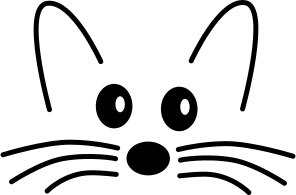
\includegraphics[width=1.4em]{squeak-logo}}}
\newcommand{\dothis}[1]{%
	\medskip
	\noindent\dothisicon
	\ifx#1\empty\else\quad\emph{#1}\fi
	\par\smallskip\nopagebreak}
% NB: To use this in an individual chapter, you must set:
%\graphicspath{{figures/} {../figures/}}
% at the head of the chapter.  Don't forget the final /
%=============================================================
%:Reader hints (hint)
%
% Indicates a non-obvious consequence 
\newcommand{\hint}[1]{\vspace{1ex}\noindent\fbox{\textsc{Astuce}} \emph{#1}}
%=================================================================
% graphics for Morphic handles
\newcommand{\grabHandle}{\raisebox{-0.2ex}{
\includegraphics[width=1em]{blackHandle}}}
\newcommand{\moveHandle}{\raisebox{-0.2ex}{
\includegraphics[width=1em]{moveHandle}}}
\newcommand{\debugHandle}{\raisebox{-0.2ex}{
\includegraphics[width=1em]{debugHandle}}}
% squeak-fr (added for Morphic handles)
\newcommand{\rotateHandle}{\raisebox{-0.2ex}{
\includegraphics[width=1em]{rotateHandle}}}
\newcommand{\viewerHandle}{\raisebox{-0.2ex}{
\includegraphics[width=1em]{viewerHandle}}}
% squeak-fr (add cloverHandle to use \clover in QuickTour.tex as alias
% todo 

%=============================================================
%:Highlighting Important stuff (doublebox)
%
% From Seaside book ...
\newsavebox{\SavedText}
\newlength{\InnerBoxRule}\setlength{\InnerBoxRule}{.75\fboxrule}
\newlength{\OuterBoxRule}\setlength{\OuterBoxRule}{1.5\fboxrule}
\newlength{\BoxSeparation}\setlength{\BoxSeparation}{1.5\fboxrule}
\addtolength{\BoxSeparation}{.5pt}
\newlength{\SaveBoxSep}\setlength{\SaveBoxSep}{2\fboxsep}
%
\newenvironment{doublebox}{\begin{lrbox}{\SavedText}
    \begin{minipage}{.75\textwidth}}
    {\end{minipage}\end{lrbox}\begin{center}
    \setlength{\fboxsep}{\BoxSeparation}\setlength{\fboxrule}{\OuterBoxRule}
    \fbox{\setlength{\fboxsep}{\SaveBoxSep}\setlength{\fboxrule}{\InnerBoxRule}%
      \fbox{\usebox{\SavedText}}}
  \end{center}}
% Use this:
\newcommand{\important}[1]{\begin{doublebox}#1\end{doublebox}}
%=============================================================
%:Section depth
\setcounter{secnumdepth}{2}
%% for this to happen start the file with
%\ifx\wholebook\relax\else
%% $Author$ Martial
% $Date$ Wed Oct 10 13:34:55 CEST 2007
% $Revision$ source: SBE 12715 
% Last Changed Date: 2007-10-08 21:32:45 +0200 (Mon, 08 Oct 2007)
%=============================================================
% NB: documentclass must be set in main document.
% Allows book to be generated in multiple formats.
%=============================================================
%:Packages
\usepackage[french]{babel}
\usepackage[T1]{fontenc}  %%%%%% really important to get the code directly in the text!
\usepackage{lmodern}
%\usepackage[scaled=0.85]{bookmanx} % needs another scale factor if used with \renewcommand{\sfdefault}{cmbr}
\usepackage{palatino}
\usepackage[scaled=0.85]{helvet}
\usepackage{microtype}
\usepackage{graphicx}
\usepackage{theorem}
\usepackage[utf8]{inputenc}
% ON: pdfsync breaks the use of p{width} for tabular columns!
\ifdefined\usepdfsync\usepackage{pdfsync}\fi % Requires texlive 2007
%=============================================================
%:More packages
%Stef should check which ones are used!
%\usepackage{picinpar}
%\usepackage{layout}
%\usepackage{color}
%\usepackage{enum}
%\usepackage{a4wide}
% \usepackage{fancyhdr}
\usepackage{ifthen}
\usepackage{float}
\usepackage{longtable}
\usepackage{makeidx}
\usepackage[nottoc]{tocbibind}
\usepackage{multicol}
\usepackage{booktabs}	% book-style tables
\usepackage{topcapt}	% enables \topcaption
\usepackage{multirow}
\usepackage{tabularx}
%\usepackage[bottom]{footmisc}
\usepackage{xspace}
\usepackage{alltt}
\usepackage{amssymb,textcomp}
\usepackage[usenames,dvipsnames]{color}
%\usepackage{colortbl}
\usepackage[hang]{subfigure}\makeatletter\def\p@subfigure{\thefigure\,}\makeatother
\usepackage{rotating}
\usepackage{enumitem}	% apb: allows more control over tags in enumerations
\usepackage{verbatim}     % for comment environment
\usepackage{varioref}	% for page references that work
\labelformat{footnote}{\thechapter--#1} % to distinguish citations from jurabib
\usepackage{needspace}
\usepackage{isodateo} % enable \isodate
\usepackage[newparttoc]{titlesec}
\usepackage{titletoc}
\usepackage{eurosym}
\usepackage{wrapfig}

\usepackage[
	super,
	citefull=first,
	authorformat={allreversed,and},
	titleformat={commasep,italic}
]{jurabib} % citations as footnotes
\usepackage[
	colorlinks=true,
	linkcolor=black,
	urlcolor=black,
	citecolor=black
]{hyperref}   % should come last

%=============================================================
%:URL style
\makeatletter

\def\url@leostyle{%
  \@ifundefined{selectfont}{\def\UrlFont{\sf}}{\def\UrlFont{\sffamily}}}
% ajouter par Martial pour \traduit (met une dague dans les \doublebox
\def\thempfootnote{\fnsymbol{mpfootnote}}

\makeatother
% Now actually use the newly defined style.
\urlstyle{leo}
%=============================================================
%:Booleans
\newboolean{lulu}
\setboolean{lulu}{false}
\newcommand{\ifluluelse}[2]{\ifthenelse{\boolean{lulu}}{#1}{#2}}
%=============================================================
%:Names
\newcommand{\SUnit}{SUnit\xspace}
\newcommand{\sunit}{SUnit\xspace}
\newcommand{\xUnit}{$x$Unit\xspace}
\newcommand{\JUnit}{JUnit\xspace}
%\newcommand{\XP}{eXtreme Programming\xspace}
\newcommand{\st}{Smalltalk\xspace}
\newcommand{\Squeak}{Squeak\xspace}
\newcommand{\sq}{Squeak\xspace}
\newcommand{\sqmap}{SqueakMap\xspace}
\newcommand{\squeak}{Squeak\xspace}
%\newcommand{\sbe}{\url{scg.unibe.ch/SBE}\xspace}
%\newcommand{\sbe}{\url{squeakbyexample.org}\xspace}
\newcommand{\sbe}{\url{SqueakByExample.org}\xspace}
% squeak-fr: adresse de la version francaise
\newcommand{\spe}{\url{SqueakByExample.org}\xspace} % ?/FR
\newcommand{\sba}{\url{SquareBracketAssociates.org}\xspace}

% squeak-fr: ajout de la \squeakdev pour eviter les problemes de
% changements d'url rencontres dans la VO:
\newcommand{\squeakdev}{\url{www.squeaksource.com/ImageForDevelopers}\xspace} %ou
%\newcommand{\squeakdev}{\url{squeak.ofset.org/squeak-dev}\xspace}

%=============================================================
%:Editorial comment macros
\newcommand{\nnbb}[2]{
    \fbox{\bfseries\sffamily\scriptsize#1}
    {\sf\small$\blacktriangleright$\textit{#2}$\blacktriangleleft$}
   }
\newcommand{\ab}[1]{\nnbb{Andrew}{#1}}
\newcommand{\sd}[1]{\nnbb{St\'{e}f}{#1}}
\newcommand{\md}[1]{\nnbb{Marcus}{#1}}
\newcommand{\on}[1]{\nnbb{Oscar}{#1}}
\newcommand{\damien}[1]{\nnbb{Damien}{#1}}
\newcommand{\lr}[1]{\nnbb{Lukas}{#1}}
\newcommand{\orla}[1]{\nnbb{Orla}{#1}}
%\newcommand{\here}{\nnbb{CONTINUE}{HERE}}
\newcommand{\here}{\nnbb{CONTINUE}{ICI}}

%=============================================================
%:Abbreviation macros
\newcommand{\ie}{\emph{c-\`a-d.}\xspace}
\newcommand{\cad}{\emph{c-\`a-d.}\xspace}
%\newcommand{\eg}{\emph{e.g.},\xspace}
\newcommand{\eg}{\emph{par ex.},\xspace}
\newcommand{\parex}{\emph{par ex.},\xspace}
\newcommand{\etc}{etc\xspace}
%=============================================================
%:Cross reference macros

% [squeak-fr] martial: remarquez les articles devant les noms
\newcommand{\charef}[1]{le chapitre~\ref{cha:#1}\xspace}
% note de martial: utilise dans chapitre Syntax.tex: a redefinir
\newcommand{\charefs}[2]{les chapitres~\ref{cha:#1} et \ref{cha:#2}\xspace}
\newcommand{\secref}[1]{la section~\ref{sec:#1}\xspace}
\newcommand{\figref}[1]{la figure~\ref{fig:#1}\xspace}
\newcommand{\Figref}[1]{La figure~\ref{fig:#1}\xspace}
\newcommand{\appref}[1]{l'annexe~\ref{app:#1}\xspace}
\newcommand{\tabref}[1]{la table~\ref{tab:#1}\xspace}
% defini pour le chapitre Messages.tex
\newcommand{\Tabref}[1]{La table~\ref{tab:#1}\xspace}

% APB: I removed trailing \xspace commands from these macros because
% \xspace mostly doesn't work.  If you want a space after your
% references, type one!
% ON: xspace has always worked just fine for me!  Please leave them in.
%
\newcommand{\ruleref}[1]{\ref{rule:#1}\xspace}
%
\newcommand{\egref}[1]{exemple~\ref{eg:#1}\xspace}
\newcommand{\Egref}[1]{Exemple~\ref{eg:#1}\xspace}
%
\newcommand{\scrref}[1]{script~\ref{scr:#1}\xspace}
\newcommand{\Scrref}[1]{Script~\ref{scr:#1}\xspace}
% t = the
\newcommand{\tscrref}[1]{le script~\ref{scr:#1}\xspace}
\newcommand{\Tscrref}[1]{Le script~\ref{scr:#1}\xspace}
%
\newcommand{\mthref}[1]{m\'ethode~\ref{mth:#1}\xspace}
\newcommand{\mthsref}[1]{m\'ethodes~\ref{mth:#1}\xspace}
\newcommand{\Mthref}[1]{M\'ethode~\ref{mth:#1}\xspace}
\newcommand{\tmthref}[1]{la m\'ethode~\ref{mth:#1}\xspace}
\newcommand{\Tmthref}[1]{La m\'ethode~\ref{mth:#1}\xspace}
%
\newcommand{\clsref}[1]{classe~\ref{cls:#1}\xspace}
\newcommand{\tclsref}[1]{la classe~\ref{cls:#1}\xspace}
\newcommand{\Tclsref}[1]{La classe~\ref{cls:#1}\xspace}
%=============================================================
%:Menu item macro
% for menu items, so we can change our minds on how to print them! (apb)
\definecolor{lightgray}{gray}{0.89}
\newcommand{\menu}[1]{{%
	\setlength{\fboxsep}{0pt}%
	\colorbox{lightgray}{{{\upshape\sffamily\strut \,#1\,}}}}}
% \newcommand{\menu}[1]{{%
% 	\fontfamily{lmr}\selectfont
% 	\upshape\textlangle{\sffamily #1}\textrangle}}
% For submenu items:
\newcommand{\go}{\,$\triangleright$\,}
% \newcommand{\go}{\,$\blacktriangleright$\,}
% For keyboard shortcuts:
%\newcommand{\short}[1]{\mbox{$\langle${\sc CMD}$\rangle$-#1}\xspace}
\newcommand{\short}[1]{\mbox{{\sc cmd}\hspace{0.08em}--\hspace{0.09em}#1}\xspace}
% For buttons:
\newcommand{\button}[1]{{%
	\setlength{\fboxsep}{0pt}%
	\fbox{{\upshape\sffamily\strut \,#1\,}}}}
\newcommand{\toolsflap}{l'onglet \textit{Tools}\xspace}
%=============================================================
%:Reader cues (do this)
%
% Indicate something the reader should try out.
\newcommand{\dothisicon}{\raisebox{-.5ex}{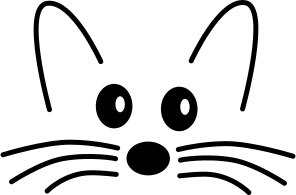
\includegraphics[width=1.4em]{squeak-logo}}}
\newcommand{\dothis}[1]{%
	\medskip
	\noindent\dothisicon
	\ifx#1\empty\else\quad\emph{#1}\fi
	\par\smallskip\nopagebreak}
% NB: To use this in an individual chapter, you must set:
%\graphicspath{{figures/} {../figures/}}
% at the head of the chapter.  Don't forget the final /
%=============================================================
%:Reader hints (hint)
%
% Indicates a non-obvious consequence 
\newcommand{\hint}[1]{\vspace{1ex}\noindent\fbox{\textsc{Astuce}} \emph{#1}}
%=================================================================
% graphics for Morphic handles
\newcommand{\grabHandle}{\raisebox{-0.2ex}{
\includegraphics[width=1em]{blackHandle}}}
\newcommand{\moveHandle}{\raisebox{-0.2ex}{
\includegraphics[width=1em]{moveHandle}}}
\newcommand{\debugHandle}{\raisebox{-0.2ex}{
\includegraphics[width=1em]{debugHandle}}}
% squeak-fr (added for Morphic handles)
\newcommand{\rotateHandle}{\raisebox{-0.2ex}{
\includegraphics[width=1em]{rotateHandle}}}
\newcommand{\viewerHandle}{\raisebox{-0.2ex}{
\includegraphics[width=1em]{viewerHandle}}}
% squeak-fr (add cloverHandle to use \clover in QuickTour.tex as alias
% todo 

%=============================================================
%:Highlighting Important stuff (doublebox)
%
% From Seaside book ...
\newsavebox{\SavedText}
\newlength{\InnerBoxRule}\setlength{\InnerBoxRule}{.75\fboxrule}
\newlength{\OuterBoxRule}\setlength{\OuterBoxRule}{1.5\fboxrule}
\newlength{\BoxSeparation}\setlength{\BoxSeparation}{1.5\fboxrule}
\addtolength{\BoxSeparation}{.5pt}
\newlength{\SaveBoxSep}\setlength{\SaveBoxSep}{2\fboxsep}
%
\newenvironment{doublebox}{\begin{lrbox}{\SavedText}
    \begin{minipage}{.75\textwidth}}
    {\end{minipage}\end{lrbox}\begin{center}
    \setlength{\fboxsep}{\BoxSeparation}\setlength{\fboxrule}{\OuterBoxRule}
    \fbox{\setlength{\fboxsep}{\SaveBoxSep}\setlength{\fboxrule}{\InnerBoxRule}%
      \fbox{\usebox{\SavedText}}}
  \end{center}}
% Use this:
\newcommand{\important}[1]{\begin{doublebox}#1\end{doublebox}}
%=============================================================
%:Section depth
\setcounter{secnumdepth}{2}
%% for this to happen start the file with
%\ifx\wholebook\relax\else
%% $Author$ Martial
% $Date$ Wed Oct 10 13:34:55 CEST 2007
% $Revision$ source: SBE 12715 
% Last Changed Date: 2007-10-08 21:32:45 +0200 (Mon, 08 Oct 2007)
%=============================================================
% NB: documentclass must be set in main document.
% Allows book to be generated in multiple formats.
%=============================================================
%:Packages
\usepackage[french]{babel}
\usepackage[T1]{fontenc}  %%%%%% really important to get the code directly in the text!
\usepackage{lmodern}
%\usepackage[scaled=0.85]{bookmanx} % needs another scale factor if used with \renewcommand{\sfdefault}{cmbr}
\usepackage{palatino}
\usepackage[scaled=0.85]{helvet}
\usepackage{microtype}
\usepackage{graphicx}
\usepackage{theorem}
\usepackage[utf8]{inputenc}
% ON: pdfsync breaks the use of p{width} for tabular columns!
\ifdefined\usepdfsync\usepackage{pdfsync}\fi % Requires texlive 2007
%=============================================================
%:More packages
%Stef should check which ones are used!
%\usepackage{picinpar}
%\usepackage{layout}
%\usepackage{color}
%\usepackage{enum}
%\usepackage{a4wide}
% \usepackage{fancyhdr}
\usepackage{ifthen}
\usepackage{float}
\usepackage{longtable}
\usepackage{makeidx}
\usepackage[nottoc]{tocbibind}
\usepackage{multicol}
\usepackage{booktabs}	% book-style tables
\usepackage{topcapt}	% enables \topcaption
\usepackage{multirow}
\usepackage{tabularx}
%\usepackage[bottom]{footmisc}
\usepackage{xspace}
\usepackage{alltt}
\usepackage{amssymb,textcomp}
\usepackage[usenames,dvipsnames]{color}
%\usepackage{colortbl}
\usepackage[hang]{subfigure}\makeatletter\def\p@subfigure{\thefigure\,}\makeatother
\usepackage{rotating}
\usepackage{enumitem}	% apb: allows more control over tags in enumerations
\usepackage{verbatim}     % for comment environment
\usepackage{varioref}	% for page references that work
\labelformat{footnote}{\thechapter--#1} % to distinguish citations from jurabib
\usepackage{needspace}
\usepackage{isodateo} % enable \isodate
\usepackage[newparttoc]{titlesec}
\usepackage{titletoc}
\usepackage{eurosym}
\usepackage{wrapfig}

\usepackage[
	super,
	citefull=first,
	authorformat={allreversed,and},
	titleformat={commasep,italic}
]{jurabib} % citations as footnotes
\usepackage[
	colorlinks=true,
	linkcolor=black,
	urlcolor=black,
	citecolor=black
]{hyperref}   % should come last

%=============================================================
%:URL style
\makeatletter

\def\url@leostyle{%
  \@ifundefined{selectfont}{\def\UrlFont{\sf}}{\def\UrlFont{\sffamily}}}
% ajouter par Martial pour \traduit (met une dague dans les \doublebox
\def\thempfootnote{\fnsymbol{mpfootnote}}

\makeatother
% Now actually use the newly defined style.
\urlstyle{leo}
%=============================================================
%:Booleans
\newboolean{lulu}
\setboolean{lulu}{false}
\newcommand{\ifluluelse}[2]{\ifthenelse{\boolean{lulu}}{#1}{#2}}
%=============================================================
%:Names
\newcommand{\SUnit}{SUnit\xspace}
\newcommand{\sunit}{SUnit\xspace}
\newcommand{\xUnit}{$x$Unit\xspace}
\newcommand{\JUnit}{JUnit\xspace}
%\newcommand{\XP}{eXtreme Programming\xspace}
\newcommand{\st}{Smalltalk\xspace}
\newcommand{\Squeak}{Squeak\xspace}
\newcommand{\sq}{Squeak\xspace}
\newcommand{\sqmap}{SqueakMap\xspace}
\newcommand{\squeak}{Squeak\xspace}
%\newcommand{\sbe}{\url{scg.unibe.ch/SBE}\xspace}
%\newcommand{\sbe}{\url{squeakbyexample.org}\xspace}
\newcommand{\sbe}{\url{SqueakByExample.org}\xspace}
% squeak-fr: adresse de la version francaise
\newcommand{\spe}{\url{SqueakByExample.org}\xspace} % ?/FR
\newcommand{\sba}{\url{SquareBracketAssociates.org}\xspace}

% squeak-fr: ajout de la \squeakdev pour eviter les problemes de
% changements d'url rencontres dans la VO:
\newcommand{\squeakdev}{\url{www.squeaksource.com/ImageForDevelopers}\xspace} %ou
%\newcommand{\squeakdev}{\url{squeak.ofset.org/squeak-dev}\xspace}

%=============================================================
%:Editorial comment macros
\newcommand{\nnbb}[2]{
    \fbox{\bfseries\sffamily\scriptsize#1}
    {\sf\small$\blacktriangleright$\textit{#2}$\blacktriangleleft$}
   }
\newcommand{\ab}[1]{\nnbb{Andrew}{#1}}
\newcommand{\sd}[1]{\nnbb{St\'{e}f}{#1}}
\newcommand{\md}[1]{\nnbb{Marcus}{#1}}
\newcommand{\on}[1]{\nnbb{Oscar}{#1}}
\newcommand{\damien}[1]{\nnbb{Damien}{#1}}
\newcommand{\lr}[1]{\nnbb{Lukas}{#1}}
\newcommand{\orla}[1]{\nnbb{Orla}{#1}}
%\newcommand{\here}{\nnbb{CONTINUE}{HERE}}
\newcommand{\here}{\nnbb{CONTINUE}{ICI}}

%=============================================================
%:Abbreviation macros
\newcommand{\ie}{\emph{c-\`a-d.}\xspace}
\newcommand{\cad}{\emph{c-\`a-d.}\xspace}
%\newcommand{\eg}{\emph{e.g.},\xspace}
\newcommand{\eg}{\emph{par ex.},\xspace}
\newcommand{\parex}{\emph{par ex.},\xspace}
\newcommand{\etc}{etc\xspace}
%=============================================================
%:Cross reference macros

% [squeak-fr] martial: remarquez les articles devant les noms
\newcommand{\charef}[1]{le chapitre~\ref{cha:#1}\xspace}
% note de martial: utilise dans chapitre Syntax.tex: a redefinir
\newcommand{\charefs}[2]{les chapitres~\ref{cha:#1} et \ref{cha:#2}\xspace}
\newcommand{\secref}[1]{la section~\ref{sec:#1}\xspace}
\newcommand{\figref}[1]{la figure~\ref{fig:#1}\xspace}
\newcommand{\Figref}[1]{La figure~\ref{fig:#1}\xspace}
\newcommand{\appref}[1]{l'annexe~\ref{app:#1}\xspace}
\newcommand{\tabref}[1]{la table~\ref{tab:#1}\xspace}
% defini pour le chapitre Messages.tex
\newcommand{\Tabref}[1]{La table~\ref{tab:#1}\xspace}

% APB: I removed trailing \xspace commands from these macros because
% \xspace mostly doesn't work.  If you want a space after your
% references, type one!
% ON: xspace has always worked just fine for me!  Please leave them in.
%
\newcommand{\ruleref}[1]{\ref{rule:#1}\xspace}
%
\newcommand{\egref}[1]{exemple~\ref{eg:#1}\xspace}
\newcommand{\Egref}[1]{Exemple~\ref{eg:#1}\xspace}
%
\newcommand{\scrref}[1]{script~\ref{scr:#1}\xspace}
\newcommand{\Scrref}[1]{Script~\ref{scr:#1}\xspace}
% t = the
\newcommand{\tscrref}[1]{le script~\ref{scr:#1}\xspace}
\newcommand{\Tscrref}[1]{Le script~\ref{scr:#1}\xspace}
%
\newcommand{\mthref}[1]{m\'ethode~\ref{mth:#1}\xspace}
\newcommand{\mthsref}[1]{m\'ethodes~\ref{mth:#1}\xspace}
\newcommand{\Mthref}[1]{M\'ethode~\ref{mth:#1}\xspace}
\newcommand{\tmthref}[1]{la m\'ethode~\ref{mth:#1}\xspace}
\newcommand{\Tmthref}[1]{La m\'ethode~\ref{mth:#1}\xspace}
%
\newcommand{\clsref}[1]{classe~\ref{cls:#1}\xspace}
\newcommand{\tclsref}[1]{la classe~\ref{cls:#1}\xspace}
\newcommand{\Tclsref}[1]{La classe~\ref{cls:#1}\xspace}
%=============================================================
%:Menu item macro
% for menu items, so we can change our minds on how to print them! (apb)
\definecolor{lightgray}{gray}{0.89}
\newcommand{\menu}[1]{{%
	\setlength{\fboxsep}{0pt}%
	\colorbox{lightgray}{{{\upshape\sffamily\strut \,#1\,}}}}}
% \newcommand{\menu}[1]{{%
% 	\fontfamily{lmr}\selectfont
% 	\upshape\textlangle{\sffamily #1}\textrangle}}
% For submenu items:
\newcommand{\go}{\,$\triangleright$\,}
% \newcommand{\go}{\,$\blacktriangleright$\,}
% For keyboard shortcuts:
%\newcommand{\short}[1]{\mbox{$\langle${\sc CMD}$\rangle$-#1}\xspace}
\newcommand{\short}[1]{\mbox{{\sc cmd}\hspace{0.08em}--\hspace{0.09em}#1}\xspace}
% For buttons:
\newcommand{\button}[1]{{%
	\setlength{\fboxsep}{0pt}%
	\fbox{{\upshape\sffamily\strut \,#1\,}}}}
\newcommand{\toolsflap}{l'onglet \textit{Tools}\xspace}
%=============================================================
%:Reader cues (do this)
%
% Indicate something the reader should try out.
\newcommand{\dothisicon}{\raisebox{-.5ex}{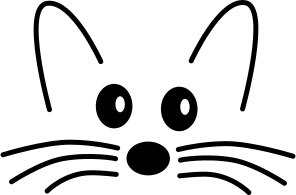
\includegraphics[width=1.4em]{squeak-logo}}}
\newcommand{\dothis}[1]{%
	\medskip
	\noindent\dothisicon
	\ifx#1\empty\else\quad\emph{#1}\fi
	\par\smallskip\nopagebreak}
% NB: To use this in an individual chapter, you must set:
%\graphicspath{{figures/} {../figures/}}
% at the head of the chapter.  Don't forget the final /
%=============================================================
%:Reader hints (hint)
%
% Indicates a non-obvious consequence 
\newcommand{\hint}[1]{\vspace{1ex}\noindent\fbox{\textsc{Astuce}} \emph{#1}}
%=================================================================
% graphics for Morphic handles
\newcommand{\grabHandle}{\raisebox{-0.2ex}{
\includegraphics[width=1em]{blackHandle}}}
\newcommand{\moveHandle}{\raisebox{-0.2ex}{
\includegraphics[width=1em]{moveHandle}}}
\newcommand{\debugHandle}{\raisebox{-0.2ex}{
\includegraphics[width=1em]{debugHandle}}}
% squeak-fr (added for Morphic handles)
\newcommand{\rotateHandle}{\raisebox{-0.2ex}{
\includegraphics[width=1em]{rotateHandle}}}
\newcommand{\viewerHandle}{\raisebox{-0.2ex}{
\includegraphics[width=1em]{viewerHandle}}}
% squeak-fr (add cloverHandle to use \clover in QuickTour.tex as alias
% todo 

%=============================================================
%:Highlighting Important stuff (doublebox)
%
% From Seaside book ...
\newsavebox{\SavedText}
\newlength{\InnerBoxRule}\setlength{\InnerBoxRule}{.75\fboxrule}
\newlength{\OuterBoxRule}\setlength{\OuterBoxRule}{1.5\fboxrule}
\newlength{\BoxSeparation}\setlength{\BoxSeparation}{1.5\fboxrule}
\addtolength{\BoxSeparation}{.5pt}
\newlength{\SaveBoxSep}\setlength{\SaveBoxSep}{2\fboxsep}
%
\newenvironment{doublebox}{\begin{lrbox}{\SavedText}
    \begin{minipage}{.75\textwidth}}
    {\end{minipage}\end{lrbox}\begin{center}
    \setlength{\fboxsep}{\BoxSeparation}\setlength{\fboxrule}{\OuterBoxRule}
    \fbox{\setlength{\fboxsep}{\SaveBoxSep}\setlength{\fboxrule}{\InnerBoxRule}%
      \fbox{\usebox{\SavedText}}}
  \end{center}}
% Use this:
\newcommand{\important}[1]{\begin{doublebox}#1\end{doublebox}}
%=============================================================
%:Section depth
\setcounter{secnumdepth}{2}
%% for this to happen start the file with
%\ifx\wholebook\relax\else
%\input{../common.tex}
%\begin{document}
%\fi
% and terminate by
% \ifx\wholebook\relax\else\end{document}\fi

\DeclareGraphicsExtensions{.pdf, .jpg, .png}
%=============================================================
%:PDF setup
\hypersetup{
%   a4paper,
%   pdfstartview=FitV,
%   colorlinks,
%   linkcolor=darkblue,
%   citecolor=darkblue,
%   pdftitle={Squeak by Example},
pdftitle={Squeak par l'exemple},
   pdfauthor={Andrew Black, St\'ephane Ducasse,	Oscar Nierstrasz,
Damien Pollet},
   pdfkeywords={Smalltalk, Squeak, Programmation Orient\'ee Objet},
pdfsubject={Informatique, Computer Science}
}
%=============================================================
%:Page layout and appearance
%
% \renewcommand{\headrulewidth}{0pt}
\renewcommand{\chaptermark}[1]{\markboth{#1}{}}
\renewcommand{\sectionmark}[1]{\markright{\thesection\ #1}}
\renewpagestyle{plain}[\small\itshape]{%
	\setheadrule{0pt}%
	\sethead[\thepage][][]{}{}{\thepage}%
	\setfoot[][][]{}{}{}}
\renewpagestyle{headings}[\small\itshape]{%
	\setheadrule{0pt}%
	\setmarks{chapter}{section}%
	\sethead[\thepage][][\chaptertitle]{\sectiontitle}{}{\thepage}%
	\setfoot[][][]{}{}{}}
%=============================================================
%:Title section setup and TOC numbering depth
\setcounter{secnumdepth}{1}
\setcounter{tocdepth}{1}
\titleformat{\part}[display]{\centering}{\huge\partname\ \thepart}{1em}{\Huge\textbf}[]
\titleformat{\chapter}[display]{}{\huge\chaptertitlename\ \thechapter}{1em}{\Huge\raggedright\textbf}[]
\titlecontents{part}[3pc]{%
		\pagebreak[2]\addvspace{1em plus.4em minus.2em}%
		\leavevmode\large\bfseries}
	{\contentslabel{3pc}}{\hspace*{-3pc}}
	{}[\nopagebreak]
\titlecontents{chapter}[3pc]{%
		\pagebreak[0]\addvspace{1em plus.2em minus.2em}%
		\leavevmode\bfseries}
	{\contentslabel{3pc}}{}
	{\hfill\contentspage}[\nopagebreak]
\dottedcontents{section}[3pc]{}{3pc}{1pc}
\dottedcontents{subsection}[3pc]{}{0pc}{1pc}
% \dottedcontents{subsection}[4.5em]{}{0pt}{1pc}
% Make \cleardoublepage insert really blank pages http://www.tex.ac.uk/cgi-bin/texfaq2html?label=reallyblank
\let\origdoublepage\cleardoublepage
\newcommand{\clearemptydoublepage}{%
  \clearpage
  {\pagestyle{empty}\origdoublepage}}
\let\cleardoublepage\clearemptydoublepage % see http://www.tex.ac.uk/cgi-bin/texfaq2html?label=patch
%=============================================================
%:FAQ macros (for FAQ chapter)
\newtheorem{faq}{FAQ}
\newcommand{\answer}{\paragraph{R\'eponse}\ }
%=============================================================
%:Listings package configuration
\usepackage{listings}
\newcommand{\caret}{\makebox{\raisebox{0.4ex}{\footnotesize{$\wedge$}}}}
\lstdefinelanguage{Smalltalk}{
%  morekeywords={self,super,true,false,nil,thisContext}, % This is overkill
  morestring=[d]',
  morecomment=[s]{"}{"},
  alsoletter={\#:},
  escapechar={!},
  escapebegin=\itshape, % comment-like by default (Martial 11/2007)
  literate=
    {BANG}{!}1
    {UNDERSCORE}{\_}1
    {\\st}{Smalltalk}9 % convenience -- in case \st occurs in code
    % {'}{{\textquotesingle}}1 % replaced by upquote=true in \lstset
    {_}{{$\leftarrow$}}1
    {>>>}{{\sep}}1
    {^}{{$\uparrow$}}1
    {~}{{$\sim$}}1
    {-}{{\sf -\hspace{-0.13em}-}}1  % the goal is to make - the same width as +
    {+}{\raisebox{0.08ex}{+}}1		% and to raise + off the baseline to match -
    {-->}{{\quad$\longrightarrow$\quad}}3
	, % Don't forget the comma at the end!
  tabsize=4
}[keywords,comments,strings]
% ajout pour les échappements dans les codes
% indispensable pour mettre le code en emphase (cf. Model.tex) 
\newcommand{\codeify}[1]{\NoAutoSpaceBeforeFDP#1\AutoSpaceBeforeFDP}
\newcommand{\normcomment}[1]{\emph{#1}} %cf. Streams
\newcommand{\normcode}[1]{\emph{\codeify{#1}}} %cf. Streams
\newcommand{\emcode}[1]{\textbf{\normcode{#1}}} % Martial 11/2007
\lstset{language=Smalltalk,
	basicstyle=\sffamily,
	keywordstyle=\color{black}\bfseries,
	% stringstyle=\ttfamily, % Ugly! do we really want this? -- on
	%commentstyle=\itshape,
	mathescape=true,
	showstringspaces=false,
	keepspaces=true,
	breaklines=true,
	breakautoindent=true,
	lineskip={-1pt}, % Ugly hack
	upquote=true, % straight quote; requires textcomp package
	columns=fullflexible} % no fixed width fonts
% In-line code (literal)
% Normally use this for all in-line code:
\newcommand{\ct}{\lstinline[mathescape=false,basicstyle={\sffamily\upshape}]}
% apb 2007.8.28 added the \upshape declaration to avoid getting italicized code in \dothis{ } sections.
% In-line code (latex enabled)
% Use this only in special situations where \ct does not work
% (within section headings ...):

% [squeak-fr] Modification de \lct suivant les indications de Martial Boniou
\newcommand{\lct}[1]{\textsf{\textup{\NoAutoSpaceBeforeFDP #1
\AutoSpaceBeforeFDP}}} %\xspace

% Use these for system categories and protocols:
\newcommand{\scat}[1]{\emph{\textsf{#1}}\xspace}
\newcommand{\pkg}[1]{\emph{\textsf{#1}}\xspace}
\newcommand{\prot}[1]{\emph{\textsf{#1}}\xspace}
% Code environments
% NB: the arg is for tests
% Only code and example environments may be tests
\lstnewenvironment{code}[1]{%
	\lstset{%
		frame=lines,
		mathescape=false
	}
}{}
\def\ignoredollar#1{}
%=============================================================
%:Code environments (method, script ...)
% NB: the third arg is for tests
% Only code and example environments may be tests
\lstnewenvironment{example}[3][defaultlabel]{%
	\renewcommand{\lstlistingname}{Exemple}%
	\lstset{
		frame=lines,
		mathescape=false,
		caption={\emph{#2}},
		label={eg:#1}
	}
}{}
\lstnewenvironment{script}[2][defaultlabel]{%
\renewcommand{\lstlistingname}{Script}%
	\lstset{
		frame=lines,
		mathescape=false,
		name={Script},
		caption={\emph{#2}},
		label={scr:#1}
	}
}{}
\lstnewenvironment{method}[2][defaultlabel]{%
	\renewcommand{\lstlistingname}{M\'ethode}%
	\lstset{
		frame=lines,
		mathescape=false,
		name={M\'ethode},
		caption={\emph{#2}},
		label={mth:#1}
	}
}{}
\lstnewenvironment{methods}[2][defaultlabel]{% just for multiple methods at once
	\renewcommand{\lstlistingname}{M\'ethodes}%
	\lstset{
		frame=lines,
		mathescape=false,
		name={M\'ethode},
		caption={\emph{#2}},
		label={mth:#1}
	}
}{}
\lstnewenvironment{numMethod}[2][defaultlabel]{%
	\renewcommand{\lstlistingname}{M\'ethode}%
	\lstset{
		numbers=left,
		numberstyle={\tiny\sffamily},
		frame=lines,
		mathescape=false,
		name={M\'ethode},
		caption={\emph{#2}},
		label={mth:#1}
	}
}{}
\lstnewenvironment{classdef}[2][defaultlabel]{%
	\renewcommand{\lstlistingname}{Classe}%
	\lstset{
		frame=lines,
		mathescape=false,
		name={Classe},
		caption={\emph{#2}},
		label={cls:#1}
	}
}{}
%=============================================================
%:Reserving space
% Usually need one more line than the actual lines of code
\newcommand{\needlines}[1]{\Needspace{#1\baselineskip}}
%=============================================================
%:Indexing macros
% Macros ending with "ind" generate text as well as an index entry
% Macros ending with "index" *only* generate an index entry
\newcommand{\ind}[1]{\index{#1}#1\xspace} % plain text
\newcommand{\subind}[2]{\index{#1!#2}#2\xspace} % show #2, subindex inder #1
\newcommand{\emphind}[1]{\index{#1}\emph{#1}\xspace} % emph #1
\newcommand{\emphsubind}[2]{\index{#1!#2}\emph{#2}\xspace} % show emph #2, subindex inder #1
\newcommand{\scatind}[1]{\index{#1@\textsf{#1} (cat\'egorie)}\scat{#1}} % category
\newcommand{\protind}[1]{\index{#1@\textsf{#1} (protocole)}\prot{#1}} % protocol
% \newcommand{\clsind}[1]{\index{#1@\textsf{#1} (class)}\ct{#1}\xspace}
\newcommand{\clsind}[1]{\index{#1!\#@(classe)}\ct{#1}\xspace} % class
\newcommand{\cvind}[1]{\index{#1@\textsf{#1} (variable de classe)}\ct{#1}\xspace} % class var
\newcommand{\glbind}[1]{\index{#1@\textsf{#1} (globale)}\ct{#1}\xspace} % global
\newcommand{\patind}[1]{\index{#1@#1 (patron)}\ct{#1}\xspace} % pattern
\newcommand{\pvind}[1]{\index{#1@\textsf{#1} (pseudo-variable)}\ct{#1}\xspace} % pseudo variable
% [squeak - fr]Martial: I found the following cleaner (should be
% merged in SBE for self and super)
\newcommand{\subpvindex}[2]{\index{#1@\textsf{#1} (pseudo-variable)!#2}}
\newcommand{\subpvind}[2]{\index{#1@\textsf{#1} (pseudo-variable)!#2}#2\xspace}
% used in Model.tex
\newcommand{\mthind}[2]{\index{#1!#2@\ct{#2}}\ct{#2}\xspace} % show method name only
\newcommand{\lmthind}[2]{\index{#1!#2@\ct{#2}}\lct{#2}\xspace} % show method name only
\newcommand{\cmind}[2]{\index{#1!#2@\ct{#2}}\ct{#1>>>#2}\xspace} % show class>>method
\newcommand{\toolsflapind}{\index{onglet Tools}\toolsflap} % index tools flap
% The following only generate an index entry:
% \newcommand{\clsindex}[1]{\index{#1@\textsf{#1} (class)}}
\newcommand{\clsindex}[1]{\index{#1!\#@(classe)}} % class
\newcommand{\cmindex}[2]{\index{#1!#2@\ct{#2}}} % class>>method
\newcommand{\cvindex}[1]{\index{#1@\textsf{#1} (variable de classe)}} % class var
\newcommand{\glbindex}[1]{\index{#1@\textsf{#1} (globale)}}% global
\newcommand{\pvindex}[1]{\index{#1@\textsf{#1} (pseudo-variable)}}% pseudo var
\newcommand{\seeindex}[2]{\index{#1|see{#2}}} % #1, see #2
\newcommand{\scatindex}[1]{\index{#1@\textsf{#1} (cat\'egorie)}} % category
\newcommand{\protindex}[1]{\index{#1@\textsf{#1} (protocole)}} % protocol
% How can we have the main entry page numbers in bold yet not break the hyperlink?
\newcommand{\boldidx}[1]{{\bf #1}} % breaks hyperlink
%\newcommand{\indmain}[1]{\index{#1|boldidx}#1\xspace} % plain text, main entry
%\newcommand{\emphsubindmain}[2]{\index{#1!#2|boldidx}\emph{#2}\xspace} % subindex, main entry
%\newcommand{\subindmain}[2]{\index{#1!#2|boldidx}#2\xspace} % subindex, main entry
%\newcommand{\clsindmain}[1]{\index{#1@\textsf{#1} (class)|boldidx}\ct{#1}\xspace}
%\newcommand{\clsindmain}[1]{\index{#1!\#@(class)|boldidx}\ct{#1}\xspace} % class main
%\newcommand{\indexmain}[1]{\index{#1|boldidx}} % main index entry only
\newcommand{\indmain}[1]{\index{#1}#1\xspace} 
\newcommand{\emphsubindmain}[2]{\index{#1!#2}\emph{#2}\xspace} % subindex, main entry
\newcommand{\subindmain}[2]{\index{#1!#2}#2\xspace} % subindex, main entry
%\newcommand{\clsindmain}[1]{\index{#1@\textsf{#1} (class)}\ct{#1}\xspace}
\newcommand{\clsindmain}[1]{\index{#1!\#@(classe)}\ct{#1}\xspace} % class main
\newcommand{\indexmain}[1]{\index{#1}} 
%=============================================================
%:Code macros
% some constants
\newcommand{\codesize}{\small}
\newcommand{\codefont}{\sffamily}
\newcommand{\cat}[1]{\textit{Dans la cat\'egorie #1}}%%To remove later
\newlength{\scriptindent}
\setlength{\scriptindent}{.3cm}
%% Method presentation constants
\newlength{\methodindent}
\newlength{\methodwordlength}
\newlength{\aftermethod}
\setlength{\methodindent}{0.2cm}
\settowidth{\methodwordlength}{\ M\'ethode\ }
%=============================================================
%:Smalltalk macros
%\newcommand{\sep}{{$\gg$}}
\newcommand{\sep}{\mbox{>>}}
\newcommand{\self}{\ct{self}\xspace}
\newcommand{\super}{\ct{super}\xspace}
\newcommand{\nil}{\ct{nil}\xspace}
%=============================================================
% be less conservative about float placement
% these commands are from http://www.tex.ac.uk/cgi-bin/texfaq2html?label=floats
\renewcommand{\topfraction}{.9}
\renewcommand{\bottomfraction}{.9}
\renewcommand{\textfraction}{.1}
\renewcommand{\floatpagefraction}{.85}
\renewcommand{\dbltopfraction}{.66}
\renewcommand{\dblfloatpagefraction}{.85}
\setcounter{topnumber}{9}
\setcounter{bottomnumber}{9}
\setcounter{totalnumber}{20}
\setcounter{dbltopnumber}{9}
%=============================================================
%% [Squeak-fr]
% pour identifier les zones de texte à corriger d'urgence!
\newcommand{\arevoir}[1]{#1}
% \traduit utilisé dans Model.tex
\newcommand{\traduit}[1]{\footnote[2]{#1}}
% changeset alias
\newcommand{\changeset}{\emph{change set}\xspace}
\newcommand{\changesets}{\emph{change sets}\xspace}
% callback alias
\newcommand{\callback}{\emph{callback}\xspace}
% blobmorph alias (QuickTour->blob)
\newcommand{\blobmorph}{\emph{blob}\xspace}
% repository
\newcommand{\squeaksource}{\textsf{SqueakSource}\xspace}
\newcommand{\sourceforge}{\textsf{SourceForge}\xspace}
% L'onglet Tools
\newcommand{\Toolsflap}{L'onglet \textit{Tools}\xspace}
% Mac OS X
\newcommand{\macosx}{\mbox{Mac OS X}\xspace}
% code en francais (uniquement dans le chapitre BasicClasses)
\newcommand{\codefrench}[1]{\NoAutoSpaceBeforeFDP\texttt{#1}\AutoSpaceBeforeFDP\xspace}
% mantra du modele objet (suite a l'erreur de martial)
\newcommand{\Mantra}{Tout est objet\xspace}
\newcommand{\mantra}{\MakeLowercase{\Mantra}\xspace}
% césure
\hyphenation{Omni-Brow-ser}
\hyphenation{m\'e-tho-de} % erreur de cesure commune
\hyphenation{m\'e-tho-des}
\hyphenation{e-xem-ple}
\hyphenation{en-re-gi-stre}
\hyphenation{a-na-ly-seur}
\hyphenation{glo-ba-le}
\hyphenation{fi-gu-re}
\hyphenation{vi-si-bles}
\hyphenation{cor-res-pon-dan-te}
\hyphenation{Work-space}
%=============================================================
% apb doesn't like paragraphs to run in to each other without a break
\parskip 1ex
%=============================================================
%:Stuff to check, merge or deprecate
%\setlength{\marginparsep}{2mm}
%\renewcommand{\baselinestretch}{1.1}
%=============================================================

%\begin{document}
%\fi
% and terminate by
% \ifx\wholebook\relax\else\end{document}\fi

\DeclareGraphicsExtensions{.pdf, .jpg, .png}
%=============================================================
%:PDF setup
\hypersetup{
%   a4paper,
%   pdfstartview=FitV,
%   colorlinks,
%   linkcolor=darkblue,
%   citecolor=darkblue,
%   pdftitle={Squeak by Example},
pdftitle={Squeak par l'exemple},
   pdfauthor={Andrew Black, St\'ephane Ducasse,	Oscar Nierstrasz,
Damien Pollet},
   pdfkeywords={Smalltalk, Squeak, Programmation Orient\'ee Objet},
pdfsubject={Informatique, Computer Science}
}
%=============================================================
%:Page layout and appearance
%
% \renewcommand{\headrulewidth}{0pt}
\renewcommand{\chaptermark}[1]{\markboth{#1}{}}
\renewcommand{\sectionmark}[1]{\markright{\thesection\ #1}}
\renewpagestyle{plain}[\small\itshape]{%
	\setheadrule{0pt}%
	\sethead[\thepage][][]{}{}{\thepage}%
	\setfoot[][][]{}{}{}}
\renewpagestyle{headings}[\small\itshape]{%
	\setheadrule{0pt}%
	\setmarks{chapter}{section}%
	\sethead[\thepage][][\chaptertitle]{\sectiontitle}{}{\thepage}%
	\setfoot[][][]{}{}{}}
%=============================================================
%:Title section setup and TOC numbering depth
\setcounter{secnumdepth}{1}
\setcounter{tocdepth}{1}
\titleformat{\part}[display]{\centering}{\huge\partname\ \thepart}{1em}{\Huge\textbf}[]
\titleformat{\chapter}[display]{}{\huge\chaptertitlename\ \thechapter}{1em}{\Huge\raggedright\textbf}[]
\titlecontents{part}[3pc]{%
		\pagebreak[2]\addvspace{1em plus.4em minus.2em}%
		\leavevmode\large\bfseries}
	{\contentslabel{3pc}}{\hspace*{-3pc}}
	{}[\nopagebreak]
\titlecontents{chapter}[3pc]{%
		\pagebreak[0]\addvspace{1em plus.2em minus.2em}%
		\leavevmode\bfseries}
	{\contentslabel{3pc}}{}
	{\hfill\contentspage}[\nopagebreak]
\dottedcontents{section}[3pc]{}{3pc}{1pc}
\dottedcontents{subsection}[3pc]{}{0pc}{1pc}
% \dottedcontents{subsection}[4.5em]{}{0pt}{1pc}
% Make \cleardoublepage insert really blank pages http://www.tex.ac.uk/cgi-bin/texfaq2html?label=reallyblank
\let\origdoublepage\cleardoublepage
\newcommand{\clearemptydoublepage}{%
  \clearpage
  {\pagestyle{empty}\origdoublepage}}
\let\cleardoublepage\clearemptydoublepage % see http://www.tex.ac.uk/cgi-bin/texfaq2html?label=patch
%=============================================================
%:FAQ macros (for FAQ chapter)
\newtheorem{faq}{FAQ}
\newcommand{\answer}{\paragraph{R\'eponse}\ }
%=============================================================
%:Listings package configuration
\usepackage{listings}
\newcommand{\caret}{\makebox{\raisebox{0.4ex}{\footnotesize{$\wedge$}}}}
\lstdefinelanguage{Smalltalk}{
%  morekeywords={self,super,true,false,nil,thisContext}, % This is overkill
  morestring=[d]',
  morecomment=[s]{"}{"},
  alsoletter={\#:},
  escapechar={!},
  escapebegin=\itshape, % comment-like by default (Martial 11/2007)
  literate=
    {BANG}{!}1
    {UNDERSCORE}{\_}1
    {\\st}{Smalltalk}9 % convenience -- in case \st occurs in code
    % {'}{{\textquotesingle}}1 % replaced by upquote=true in \lstset
    {_}{{$\leftarrow$}}1
    {>>>}{{\sep}}1
    {^}{{$\uparrow$}}1
    {~}{{$\sim$}}1
    {-}{{\sf -\hspace{-0.13em}-}}1  % the goal is to make - the same width as +
    {+}{\raisebox{0.08ex}{+}}1		% and to raise + off the baseline to match -
    {-->}{{\quad$\longrightarrow$\quad}}3
	, % Don't forget the comma at the end!
  tabsize=4
}[keywords,comments,strings]
% ajout pour les échappements dans les codes
% indispensable pour mettre le code en emphase (cf. Model.tex) 
\newcommand{\codeify}[1]{\NoAutoSpaceBeforeFDP#1\AutoSpaceBeforeFDP}
\newcommand{\normcomment}[1]{\emph{#1}} %cf. Streams
\newcommand{\normcode}[1]{\emph{\codeify{#1}}} %cf. Streams
\newcommand{\emcode}[1]{\textbf{\normcode{#1}}} % Martial 11/2007
\lstset{language=Smalltalk,
	basicstyle=\sffamily,
	keywordstyle=\color{black}\bfseries,
	% stringstyle=\ttfamily, % Ugly! do we really want this? -- on
	%commentstyle=\itshape,
	mathescape=true,
	showstringspaces=false,
	keepspaces=true,
	breaklines=true,
	breakautoindent=true,
	lineskip={-1pt}, % Ugly hack
	upquote=true, % straight quote; requires textcomp package
	columns=fullflexible} % no fixed width fonts
% In-line code (literal)
% Normally use this for all in-line code:
\newcommand{\ct}{\lstinline[mathescape=false,basicstyle={\sffamily\upshape}]}
% apb 2007.8.28 added the \upshape declaration to avoid getting italicized code in \dothis{ } sections.
% In-line code (latex enabled)
% Use this only in special situations where \ct does not work
% (within section headings ...):

% [squeak-fr] Modification de \lct suivant les indications de Martial Boniou
\newcommand{\lct}[1]{\textsf{\textup{\NoAutoSpaceBeforeFDP #1
\AutoSpaceBeforeFDP}}} %\xspace

% Use these for system categories and protocols:
\newcommand{\scat}[1]{\emph{\textsf{#1}}\xspace}
\newcommand{\pkg}[1]{\emph{\textsf{#1}}\xspace}
\newcommand{\prot}[1]{\emph{\textsf{#1}}\xspace}
% Code environments
% NB: the arg is for tests
% Only code and example environments may be tests
\lstnewenvironment{code}[1]{%
	\lstset{%
		frame=lines,
		mathescape=false
	}
}{}
\def\ignoredollar#1{}
%=============================================================
%:Code environments (method, script ...)
% NB: the third arg is for tests
% Only code and example environments may be tests
\lstnewenvironment{example}[3][defaultlabel]{%
	\renewcommand{\lstlistingname}{Exemple}%
	\lstset{
		frame=lines,
		mathescape=false,
		caption={\emph{#2}},
		label={eg:#1}
	}
}{}
\lstnewenvironment{script}[2][defaultlabel]{%
\renewcommand{\lstlistingname}{Script}%
	\lstset{
		frame=lines,
		mathescape=false,
		name={Script},
		caption={\emph{#2}},
		label={scr:#1}
	}
}{}
\lstnewenvironment{method}[2][defaultlabel]{%
	\renewcommand{\lstlistingname}{M\'ethode}%
	\lstset{
		frame=lines,
		mathescape=false,
		name={M\'ethode},
		caption={\emph{#2}},
		label={mth:#1}
	}
}{}
\lstnewenvironment{methods}[2][defaultlabel]{% just for multiple methods at once
	\renewcommand{\lstlistingname}{M\'ethodes}%
	\lstset{
		frame=lines,
		mathescape=false,
		name={M\'ethode},
		caption={\emph{#2}},
		label={mth:#1}
	}
}{}
\lstnewenvironment{numMethod}[2][defaultlabel]{%
	\renewcommand{\lstlistingname}{M\'ethode}%
	\lstset{
		numbers=left,
		numberstyle={\tiny\sffamily},
		frame=lines,
		mathescape=false,
		name={M\'ethode},
		caption={\emph{#2}},
		label={mth:#1}
	}
}{}
\lstnewenvironment{classdef}[2][defaultlabel]{%
	\renewcommand{\lstlistingname}{Classe}%
	\lstset{
		frame=lines,
		mathescape=false,
		name={Classe},
		caption={\emph{#2}},
		label={cls:#1}
	}
}{}
%=============================================================
%:Reserving space
% Usually need one more line than the actual lines of code
\newcommand{\needlines}[1]{\Needspace{#1\baselineskip}}
%=============================================================
%:Indexing macros
% Macros ending with "ind" generate text as well as an index entry
% Macros ending with "index" *only* generate an index entry
\newcommand{\ind}[1]{\index{#1}#1\xspace} % plain text
\newcommand{\subind}[2]{\index{#1!#2}#2\xspace} % show #2, subindex inder #1
\newcommand{\emphind}[1]{\index{#1}\emph{#1}\xspace} % emph #1
\newcommand{\emphsubind}[2]{\index{#1!#2}\emph{#2}\xspace} % show emph #2, subindex inder #1
\newcommand{\scatind}[1]{\index{#1@\textsf{#1} (cat\'egorie)}\scat{#1}} % category
\newcommand{\protind}[1]{\index{#1@\textsf{#1} (protocole)}\prot{#1}} % protocol
% \newcommand{\clsind}[1]{\index{#1@\textsf{#1} (class)}\ct{#1}\xspace}
\newcommand{\clsind}[1]{\index{#1!\#@(classe)}\ct{#1}\xspace} % class
\newcommand{\cvind}[1]{\index{#1@\textsf{#1} (variable de classe)}\ct{#1}\xspace} % class var
\newcommand{\glbind}[1]{\index{#1@\textsf{#1} (globale)}\ct{#1}\xspace} % global
\newcommand{\patind}[1]{\index{#1@#1 (patron)}\ct{#1}\xspace} % pattern
\newcommand{\pvind}[1]{\index{#1@\textsf{#1} (pseudo-variable)}\ct{#1}\xspace} % pseudo variable
% [squeak - fr]Martial: I found the following cleaner (should be
% merged in SBE for self and super)
\newcommand{\subpvindex}[2]{\index{#1@\textsf{#1} (pseudo-variable)!#2}}
\newcommand{\subpvind}[2]{\index{#1@\textsf{#1} (pseudo-variable)!#2}#2\xspace}
% used in Model.tex
\newcommand{\mthind}[2]{\index{#1!#2@\ct{#2}}\ct{#2}\xspace} % show method name only
\newcommand{\lmthind}[2]{\index{#1!#2@\ct{#2}}\lct{#2}\xspace} % show method name only
\newcommand{\cmind}[2]{\index{#1!#2@\ct{#2}}\ct{#1>>>#2}\xspace} % show class>>method
\newcommand{\toolsflapind}{\index{onglet Tools}\toolsflap} % index tools flap
% The following only generate an index entry:
% \newcommand{\clsindex}[1]{\index{#1@\textsf{#1} (class)}}
\newcommand{\clsindex}[1]{\index{#1!\#@(classe)}} % class
\newcommand{\cmindex}[2]{\index{#1!#2@\ct{#2}}} % class>>method
\newcommand{\cvindex}[1]{\index{#1@\textsf{#1} (variable de classe)}} % class var
\newcommand{\glbindex}[1]{\index{#1@\textsf{#1} (globale)}}% global
\newcommand{\pvindex}[1]{\index{#1@\textsf{#1} (pseudo-variable)}}% pseudo var
\newcommand{\seeindex}[2]{\index{#1|see{#2}}} % #1, see #2
\newcommand{\scatindex}[1]{\index{#1@\textsf{#1} (cat\'egorie)}} % category
\newcommand{\protindex}[1]{\index{#1@\textsf{#1} (protocole)}} % protocol
% How can we have the main entry page numbers in bold yet not break the hyperlink?
\newcommand{\boldidx}[1]{{\bf #1}} % breaks hyperlink
%\newcommand{\indmain}[1]{\index{#1|boldidx}#1\xspace} % plain text, main entry
%\newcommand{\emphsubindmain}[2]{\index{#1!#2|boldidx}\emph{#2}\xspace} % subindex, main entry
%\newcommand{\subindmain}[2]{\index{#1!#2|boldidx}#2\xspace} % subindex, main entry
%\newcommand{\clsindmain}[1]{\index{#1@\textsf{#1} (class)|boldidx}\ct{#1}\xspace}
%\newcommand{\clsindmain}[1]{\index{#1!\#@(class)|boldidx}\ct{#1}\xspace} % class main
%\newcommand{\indexmain}[1]{\index{#1|boldidx}} % main index entry only
\newcommand{\indmain}[1]{\index{#1}#1\xspace} 
\newcommand{\emphsubindmain}[2]{\index{#1!#2}\emph{#2}\xspace} % subindex, main entry
\newcommand{\subindmain}[2]{\index{#1!#2}#2\xspace} % subindex, main entry
%\newcommand{\clsindmain}[1]{\index{#1@\textsf{#1} (class)}\ct{#1}\xspace}
\newcommand{\clsindmain}[1]{\index{#1!\#@(classe)}\ct{#1}\xspace} % class main
\newcommand{\indexmain}[1]{\index{#1}} 
%=============================================================
%:Code macros
% some constants
\newcommand{\codesize}{\small}
\newcommand{\codefont}{\sffamily}
\newcommand{\cat}[1]{\textit{Dans la cat\'egorie #1}}%%To remove later
\newlength{\scriptindent}
\setlength{\scriptindent}{.3cm}
%% Method presentation constants
\newlength{\methodindent}
\newlength{\methodwordlength}
\newlength{\aftermethod}
\setlength{\methodindent}{0.2cm}
\settowidth{\methodwordlength}{\ M\'ethode\ }
%=============================================================
%:Smalltalk macros
%\newcommand{\sep}{{$\gg$}}
\newcommand{\sep}{\mbox{>>}}
\newcommand{\self}{\ct{self}\xspace}
\newcommand{\super}{\ct{super}\xspace}
\newcommand{\nil}{\ct{nil}\xspace}
%=============================================================
% be less conservative about float placement
% these commands are from http://www.tex.ac.uk/cgi-bin/texfaq2html?label=floats
\renewcommand{\topfraction}{.9}
\renewcommand{\bottomfraction}{.9}
\renewcommand{\textfraction}{.1}
\renewcommand{\floatpagefraction}{.85}
\renewcommand{\dbltopfraction}{.66}
\renewcommand{\dblfloatpagefraction}{.85}
\setcounter{topnumber}{9}
\setcounter{bottomnumber}{9}
\setcounter{totalnumber}{20}
\setcounter{dbltopnumber}{9}
%=============================================================
%% [Squeak-fr]
% pour identifier les zones de texte à corriger d'urgence!
\newcommand{\arevoir}[1]{#1}
% \traduit utilisé dans Model.tex
\newcommand{\traduit}[1]{\footnote[2]{#1}}
% changeset alias
\newcommand{\changeset}{\emph{change set}\xspace}
\newcommand{\changesets}{\emph{change sets}\xspace}
% callback alias
\newcommand{\callback}{\emph{callback}\xspace}
% blobmorph alias (QuickTour->blob)
\newcommand{\blobmorph}{\emph{blob}\xspace}
% repository
\newcommand{\squeaksource}{\textsf{SqueakSource}\xspace}
\newcommand{\sourceforge}{\textsf{SourceForge}\xspace}
% L'onglet Tools
\newcommand{\Toolsflap}{L'onglet \textit{Tools}\xspace}
% Mac OS X
\newcommand{\macosx}{\mbox{Mac OS X}\xspace}
% code en francais (uniquement dans le chapitre BasicClasses)
\newcommand{\codefrench}[1]{\NoAutoSpaceBeforeFDP\texttt{#1}\AutoSpaceBeforeFDP\xspace}
% mantra du modele objet (suite a l'erreur de martial)
\newcommand{\Mantra}{Tout est objet\xspace}
\newcommand{\mantra}{\MakeLowercase{\Mantra}\xspace}
% césure
\hyphenation{Omni-Brow-ser}
\hyphenation{m\'e-tho-de} % erreur de cesure commune
\hyphenation{m\'e-tho-des}
\hyphenation{e-xem-ple}
\hyphenation{en-re-gi-stre}
\hyphenation{a-na-ly-seur}
\hyphenation{glo-ba-le}
\hyphenation{fi-gu-re}
\hyphenation{vi-si-bles}
\hyphenation{cor-res-pon-dan-te}
\hyphenation{Work-space}
%=============================================================
% apb doesn't like paragraphs to run in to each other without a break
\parskip 1ex
%=============================================================
%:Stuff to check, merge or deprecate
%\setlength{\marginparsep}{2mm}
%\renewcommand{\baselinestretch}{1.1}
%=============================================================

%\begin{document}
%\fi
% and terminate by
% \ifx\wholebook\relax\else\end{document}\fi

\DeclareGraphicsExtensions{.pdf, .jpg, .png}
%=============================================================
%:PDF setup
\hypersetup{
%   a4paper,
%   pdfstartview=FitV,
%   colorlinks,
%   linkcolor=darkblue,
%   citecolor=darkblue,
%   pdftitle={Squeak by Example},
pdftitle={Squeak par l'exemple},
   pdfauthor={Andrew Black, St\'ephane Ducasse,	Oscar Nierstrasz,
Damien Pollet},
   pdfkeywords={Smalltalk, Squeak, Programmation Orient\'ee Objet},
pdfsubject={Informatique, Computer Science}
}
%=============================================================
%:Page layout and appearance
%
% \renewcommand{\headrulewidth}{0pt}
\renewcommand{\chaptermark}[1]{\markboth{#1}{}}
\renewcommand{\sectionmark}[1]{\markright{\thesection\ #1}}
\renewpagestyle{plain}[\small\itshape]{%
	\setheadrule{0pt}%
	\sethead[\thepage][][]{}{}{\thepage}%
	\setfoot[][][]{}{}{}}
\renewpagestyle{headings}[\small\itshape]{%
	\setheadrule{0pt}%
	\setmarks{chapter}{section}%
	\sethead[\thepage][][\chaptertitle]{\sectiontitle}{}{\thepage}%
	\setfoot[][][]{}{}{}}
%=============================================================
%:Title section setup and TOC numbering depth
\setcounter{secnumdepth}{1}
\setcounter{tocdepth}{1}
\titleformat{\part}[display]{\centering}{\huge\partname\ \thepart}{1em}{\Huge\textbf}[]
\titleformat{\chapter}[display]{}{\huge\chaptertitlename\ \thechapter}{1em}{\Huge\raggedright\textbf}[]
\titlecontents{part}[3pc]{%
		\pagebreak[2]\addvspace{1em plus.4em minus.2em}%
		\leavevmode\large\bfseries}
	{\contentslabel{3pc}}{\hspace*{-3pc}}
	{}[\nopagebreak]
\titlecontents{chapter}[3pc]{%
		\pagebreak[0]\addvspace{1em plus.2em minus.2em}%
		\leavevmode\bfseries}
	{\contentslabel{3pc}}{}
	{\hfill\contentspage}[\nopagebreak]
\dottedcontents{section}[3pc]{}{3pc}{1pc}
\dottedcontents{subsection}[3pc]{}{0pc}{1pc}
% \dottedcontents{subsection}[4.5em]{}{0pt}{1pc}
% Make \cleardoublepage insert really blank pages http://www.tex.ac.uk/cgi-bin/texfaq2html?label=reallyblank
\let\origdoublepage\cleardoublepage
\newcommand{\clearemptydoublepage}{%
  \clearpage
  {\pagestyle{empty}\origdoublepage}}
\let\cleardoublepage\clearemptydoublepage % see http://www.tex.ac.uk/cgi-bin/texfaq2html?label=patch
%=============================================================
%:FAQ macros (for FAQ chapter)
\newtheorem{faq}{FAQ}
\newcommand{\answer}{\paragraph{R\'eponse}\ }
%=============================================================
%:Listings package configuration
\usepackage{listings}
\newcommand{\caret}{\makebox{\raisebox{0.4ex}{\footnotesize{$\wedge$}}}}
\lstdefinelanguage{Smalltalk}{
%  morekeywords={self,super,true,false,nil,thisContext}, % This is overkill
  morestring=[d]',
  morecomment=[s]{"}{"},
  alsoletter={\#:},
  escapechar={!},
  escapebegin=\itshape, % comment-like by default (Martial 11/2007)
  literate=
    {BANG}{!}1
    {UNDERSCORE}{\_}1
    {\\st}{Smalltalk}9 % convenience -- in case \st occurs in code
    % {'}{{\textquotesingle}}1 % replaced by upquote=true in \lstset
    {_}{{$\leftarrow$}}1
    {>>>}{{\sep}}1
    {^}{{$\uparrow$}}1
    {~}{{$\sim$}}1
    {-}{{\sf -\hspace{-0.13em}-}}1  % the goal is to make - the same width as +
    {+}{\raisebox{0.08ex}{+}}1		% and to raise + off the baseline to match -
    {-->}{{\quad$\longrightarrow$\quad}}3
	, % Don't forget the comma at the end!
  tabsize=4
}[keywords,comments,strings]
% ajout pour les échappements dans les codes
% indispensable pour mettre le code en emphase (cf. Model.tex) 
\newcommand{\codeify}[1]{\NoAutoSpaceBeforeFDP#1\AutoSpaceBeforeFDP}
\newcommand{\normcomment}[1]{\emph{#1}} %cf. Streams
\newcommand{\normcode}[1]{\emph{\codeify{#1}}} %cf. Streams
\newcommand{\emcode}[1]{\textbf{\normcode{#1}}} % Martial 11/2007
\lstset{language=Smalltalk,
	basicstyle=\sffamily,
	keywordstyle=\color{black}\bfseries,
	% stringstyle=\ttfamily, % Ugly! do we really want this? -- on
	%commentstyle=\itshape,
	mathescape=true,
	showstringspaces=false,
	keepspaces=true,
	breaklines=true,
	breakautoindent=true,
	lineskip={-1pt}, % Ugly hack
	upquote=true, % straight quote; requires textcomp package
	columns=fullflexible} % no fixed width fonts
% In-line code (literal)
% Normally use this for all in-line code:
\newcommand{\ct}{\lstinline[mathescape=false,basicstyle={\sffamily\upshape}]}
% apb 2007.8.28 added the \upshape declaration to avoid getting italicized code in \dothis{ } sections.
% In-line code (latex enabled)
% Use this only in special situations where \ct does not work
% (within section headings ...):

% [squeak-fr] Modification de \lct suivant les indications de Martial Boniou
\newcommand{\lct}[1]{\textsf{\textup{\NoAutoSpaceBeforeFDP #1
\AutoSpaceBeforeFDP}}} %\xspace

% Use these for system categories and protocols:
\newcommand{\scat}[1]{\emph{\textsf{#1}}\xspace}
\newcommand{\pkg}[1]{\emph{\textsf{#1}}\xspace}
\newcommand{\prot}[1]{\emph{\textsf{#1}}\xspace}
% Code environments
% NB: the arg is for tests
% Only code and example environments may be tests
\lstnewenvironment{code}[1]{%
	\lstset{%
		frame=lines,
		mathescape=false
	}
}{}
\def\ignoredollar#1{}
%=============================================================
%:Code environments (method, script ...)
% NB: the third arg is for tests
% Only code and example environments may be tests
\lstnewenvironment{example}[3][defaultlabel]{%
	\renewcommand{\lstlistingname}{Exemple}%
	\lstset{
		frame=lines,
		mathescape=false,
		caption={\emph{#2}},
		label={eg:#1}
	}
}{}
\lstnewenvironment{script}[2][defaultlabel]{%
\renewcommand{\lstlistingname}{Script}%
	\lstset{
		frame=lines,
		mathescape=false,
		name={Script},
		caption={\emph{#2}},
		label={scr:#1}
	}
}{}
\lstnewenvironment{method}[2][defaultlabel]{%
	\renewcommand{\lstlistingname}{M\'ethode}%
	\lstset{
		frame=lines,
		mathescape=false,
		name={M\'ethode},
		caption={\emph{#2}},
		label={mth:#1}
	}
}{}
\lstnewenvironment{methods}[2][defaultlabel]{% just for multiple methods at once
	\renewcommand{\lstlistingname}{M\'ethodes}%
	\lstset{
		frame=lines,
		mathescape=false,
		name={M\'ethode},
		caption={\emph{#2}},
		label={mth:#1}
	}
}{}
\lstnewenvironment{numMethod}[2][defaultlabel]{%
	\renewcommand{\lstlistingname}{M\'ethode}%
	\lstset{
		numbers=left,
		numberstyle={\tiny\sffamily},
		frame=lines,
		mathescape=false,
		name={M\'ethode},
		caption={\emph{#2}},
		label={mth:#1}
	}
}{}
\lstnewenvironment{classdef}[2][defaultlabel]{%
	\renewcommand{\lstlistingname}{Classe}%
	\lstset{
		frame=lines,
		mathescape=false,
		name={Classe},
		caption={\emph{#2}},
		label={cls:#1}
	}
}{}
%=============================================================
%:Reserving space
% Usually need one more line than the actual lines of code
\newcommand{\needlines}[1]{\Needspace{#1\baselineskip}}
%=============================================================
%:Indexing macros
% Macros ending with "ind" generate text as well as an index entry
% Macros ending with "index" *only* generate an index entry
\newcommand{\ind}[1]{\index{#1}#1\xspace} % plain text
\newcommand{\subind}[2]{\index{#1!#2}#2\xspace} % show #2, subindex inder #1
\newcommand{\emphind}[1]{\index{#1}\emph{#1}\xspace} % emph #1
\newcommand{\emphsubind}[2]{\index{#1!#2}\emph{#2}\xspace} % show emph #2, subindex inder #1
\newcommand{\scatind}[1]{\index{#1@\textsf{#1} (cat\'egorie)}\scat{#1}} % category
\newcommand{\protind}[1]{\index{#1@\textsf{#1} (protocole)}\prot{#1}} % protocol
% \newcommand{\clsind}[1]{\index{#1@\textsf{#1} (class)}\ct{#1}\xspace}
\newcommand{\clsind}[1]{\index{#1!\#@(classe)}\ct{#1}\xspace} % class
\newcommand{\cvind}[1]{\index{#1@\textsf{#1} (variable de classe)}\ct{#1}\xspace} % class var
\newcommand{\glbind}[1]{\index{#1@\textsf{#1} (globale)}\ct{#1}\xspace} % global
\newcommand{\patind}[1]{\index{#1@#1 (patron)}\ct{#1}\xspace} % pattern
\newcommand{\pvind}[1]{\index{#1@\textsf{#1} (pseudo-variable)}\ct{#1}\xspace} % pseudo variable
% [squeak - fr]Martial: I found the following cleaner (should be
% merged in SBE for self and super)
\newcommand{\subpvindex}[2]{\index{#1@\textsf{#1} (pseudo-variable)!#2}}
\newcommand{\subpvind}[2]{\index{#1@\textsf{#1} (pseudo-variable)!#2}#2\xspace}
% used in Model.tex
\newcommand{\mthind}[2]{\index{#1!#2@\ct{#2}}\ct{#2}\xspace} % show method name only
\newcommand{\lmthind}[2]{\index{#1!#2@\ct{#2}}\lct{#2}\xspace} % show method name only
\newcommand{\cmind}[2]{\index{#1!#2@\ct{#2}}\ct{#1>>>#2}\xspace} % show class>>method
\newcommand{\toolsflapind}{\index{onglet Tools}\toolsflap} % index tools flap
% The following only generate an index entry:
% \newcommand{\clsindex}[1]{\index{#1@\textsf{#1} (class)}}
\newcommand{\clsindex}[1]{\index{#1!\#@(classe)}} % class
\newcommand{\cmindex}[2]{\index{#1!#2@\ct{#2}}} % class>>method
\newcommand{\cvindex}[1]{\index{#1@\textsf{#1} (variable de classe)}} % class var
\newcommand{\glbindex}[1]{\index{#1@\textsf{#1} (globale)}}% global
\newcommand{\pvindex}[1]{\index{#1@\textsf{#1} (pseudo-variable)}}% pseudo var
\newcommand{\seeindex}[2]{\index{#1|see{#2}}} % #1, see #2
\newcommand{\scatindex}[1]{\index{#1@\textsf{#1} (cat\'egorie)}} % category
\newcommand{\protindex}[1]{\index{#1@\textsf{#1} (protocole)}} % protocol
% How can we have the main entry page numbers in bold yet not break the hyperlink?
\newcommand{\boldidx}[1]{{\bf #1}} % breaks hyperlink
%\newcommand{\indmain}[1]{\index{#1|boldidx}#1\xspace} % plain text, main entry
%\newcommand{\emphsubindmain}[2]{\index{#1!#2|boldidx}\emph{#2}\xspace} % subindex, main entry
%\newcommand{\subindmain}[2]{\index{#1!#2|boldidx}#2\xspace} % subindex, main entry
%\newcommand{\clsindmain}[1]{\index{#1@\textsf{#1} (class)|boldidx}\ct{#1}\xspace}
%\newcommand{\clsindmain}[1]{\index{#1!\#@(class)|boldidx}\ct{#1}\xspace} % class main
%\newcommand{\indexmain}[1]{\index{#1|boldidx}} % main index entry only
\newcommand{\indmain}[1]{\index{#1}#1\xspace} 
\newcommand{\emphsubindmain}[2]{\index{#1!#2}\emph{#2}\xspace} % subindex, main entry
\newcommand{\subindmain}[2]{\index{#1!#2}#2\xspace} % subindex, main entry
%\newcommand{\clsindmain}[1]{\index{#1@\textsf{#1} (class)}\ct{#1}\xspace}
\newcommand{\clsindmain}[1]{\index{#1!\#@(classe)}\ct{#1}\xspace} % class main
\newcommand{\indexmain}[1]{\index{#1}} 
%=============================================================
%:Code macros
% some constants
\newcommand{\codesize}{\small}
\newcommand{\codefont}{\sffamily}
\newcommand{\cat}[1]{\textit{Dans la cat\'egorie #1}}%%To remove later
\newlength{\scriptindent}
\setlength{\scriptindent}{.3cm}
%% Method presentation constants
\newlength{\methodindent}
\newlength{\methodwordlength}
\newlength{\aftermethod}
\setlength{\methodindent}{0.2cm}
\settowidth{\methodwordlength}{\ M\'ethode\ }
%=============================================================
%:Smalltalk macros
%\newcommand{\sep}{{$\gg$}}
\newcommand{\sep}{\mbox{>>}}
\newcommand{\self}{\ct{self}\xspace}
\newcommand{\super}{\ct{super}\xspace}
\newcommand{\nil}{\ct{nil}\xspace}
%=============================================================
% be less conservative about float placement
% these commands are from http://www.tex.ac.uk/cgi-bin/texfaq2html?label=floats
\renewcommand{\topfraction}{.9}
\renewcommand{\bottomfraction}{.9}
\renewcommand{\textfraction}{.1}
\renewcommand{\floatpagefraction}{.85}
\renewcommand{\dbltopfraction}{.66}
\renewcommand{\dblfloatpagefraction}{.85}
\setcounter{topnumber}{9}
\setcounter{bottomnumber}{9}
\setcounter{totalnumber}{20}
\setcounter{dbltopnumber}{9}
%=============================================================
%% [Squeak-fr]
% pour identifier les zones de texte à corriger d'urgence!
\newcommand{\arevoir}[1]{#1}
% \traduit utilisé dans Model.tex
\newcommand{\traduit}[1]{\footnote[2]{#1}}
% changeset alias
\newcommand{\changeset}{\emph{change set}\xspace}
\newcommand{\changesets}{\emph{change sets}\xspace}
% callback alias
\newcommand{\callback}{\emph{callback}\xspace}
% blobmorph alias (QuickTour->blob)
\newcommand{\blobmorph}{\emph{blob}\xspace}
% repository
\newcommand{\squeaksource}{\textsf{SqueakSource}\xspace}
\newcommand{\sourceforge}{\textsf{SourceForge}\xspace}
% L'onglet Tools
\newcommand{\Toolsflap}{L'onglet \textit{Tools}\xspace}
% Mac OS X
\newcommand{\macosx}{\mbox{Mac OS X}\xspace}
% code en francais (uniquement dans le chapitre BasicClasses)
\newcommand{\codefrench}[1]{\NoAutoSpaceBeforeFDP\texttt{#1}\AutoSpaceBeforeFDP\xspace}
% mantra du modele objet (suite a l'erreur de martial)
\newcommand{\Mantra}{Tout est objet\xspace}
\newcommand{\mantra}{\MakeLowercase{\Mantra}\xspace}
% césure
\hyphenation{Omni-Brow-ser}
\hyphenation{m\'e-tho-de} % erreur de cesure commune
\hyphenation{m\'e-tho-des}
\hyphenation{e-xem-ple}
\hyphenation{en-re-gi-stre}
\hyphenation{a-na-ly-seur}
\hyphenation{glo-ba-le}
\hyphenation{fi-gu-re}
\hyphenation{vi-si-bles}
\hyphenation{cor-res-pon-dan-te}
\hyphenation{Work-space}
%=============================================================
% apb doesn't like paragraphs to run in to each other without a break
\parskip 1ex
%=============================================================
%:Stuff to check, merge or deprecate
%\setlength{\marginparsep}{2mm}
%\renewcommand{\baselinestretch}{1.1}
%=============================================================

%	\usepackage{a4wide}
% --------------------------------------------
    \graphicspath{{figures/} {../figures/}}
	\begin{document}
	\renewcommand{\nnbb}[2]{} % Disable editorial comments
	\sloppy
\fi
%=================================================================
\chapter{Le mod\`ele objet de \st}
\label{cha:SqueakModel}\label{cha:model}

Le mod\`ele de programmation de \st est simple et homog\`ene: tout est objet et les objets communiquent les uns avec les autres uniquement
via envoi de messages (nous disons aussi transmission de messages).
Cependant, ces caract\'eristiques de simplicit\'e et d'homog\'en\'eit\'e peuvent \^etre source de quelques difficult\'es pour le programmeur habitu\'e \`a d'autres langages. Dans ce chapitre nous pr\'esenterons les concepts de base du mod\`ele objet de \st; en particulier nous discuterons des cons\'equences de repr\'esenter les classes comme des objets.

%=========================================================
\section{Les r\`egles du mod\`ele}
\label{sec:rules}

Le mod\`ele objet de \st repose sur un ensemble de r\`egles simples 
qui sont appliqu\'es de mani\`ere \emph{uniforme}. Les r\`egles s'\'enoncent comme suit:

\begin{enumerate}[label={\textbf{R\`egle \arabic{*}}.}, ref={R\`egle \arabic{*}}, leftmargin=*]
\item{} \label{rule:everything}
	Tout est un objet.

\item{} \label{rule:instance}
	Tout objet est instance de classe.

\item{} \label{rule:inheritance}
	Toute classe a une super-classe.

\item{}  \label{rule:message}
	Tout se passe par envoi de messages.

\item{}  \label{rule:lookup}
	La recherche des m\'ethodes suit la cha\^ine de l'h\'eritage.

\end{enumerate}

\noindent
Prenons le temps d'\'etudier ces r\`egles en d\'etail.


%=========================================================
\section{Tout est un objet}

%\ruleref{everything}

Le mantra ``tout est un objet'' est hautement contagieux.
Apr\`es seulement peu de temps pass\'e avec \st, vous serez progressivement surpris par comment cette r\`egle simplifie tout ce que vous faites.
Par exemple, les entiers sont v\'eritablement des objets (de classe Integer). D\`es lors vous pouvez leur envoyer des messages, comme vous feriez avec n'importe quel autre objet.

\begin{code}{@TEST}
3 + 4            --> 7    "!envoie '+ 4' \`a 3, donnant 7!"
20 factorial  --> 2432902008176640000   "envoie factorial, donnant un grand nombre"
\end{code}

La repr\'esentation de \ct{20 factorial} est certainement diff\'erente de la repr\'esentation de \ct{7}, mais aucune partie du code\,---\,pas m\^eme l'impl\'ementation de 
\ct{factorial}~\footnote{En anglais, factorielle.}
\,---\,n'a besoin de le savoir puisque ce sont des objets tous deux.

\needlines{3}
La cons\'equence fondamentale de cette r\`egle pourrait s'\'enoncer ainsi:

\important{Les classes sont aussi des objets.}
Plus encore, les classes ne sont pas des objets de seconde zone: elles sont v\'eritablement des objets de premier plan auquels vous pouvez envoyer des messages, que vous pouvez inspecter, \etc.
Ainsi \squeak est vraiment un syst\`eme r\'eflexif offrant une grande expressivit\'e
aux développeurs.

En regardant plus avant dans l'impl\'ementation de \st, nous trouvons
trois sortes diff\'erentes d'objets. Il y a (1) les objets ordinaires
avec des variables d'instance pass\'ees par r\'eference; il y a (2)
\emph{les petits entiers}~\footnote{En anglais, \emph{small
    integers}.} qui sont pass\'es par valeur, et enfin, il y a (3) les
objets 
%martial: remplacement de 'indexables' (Tue Dec 25 11:37:17 CET 2007)
index\'es comme les Array (tableaux) qui ont une portion contig\"ue de m\'emoire. La beaut\'e de \st r\'eside 
dans le fait que vous n'avez aucunement \`a vous soucier des diff\'erences entre ces trois types
d'objet.


%=========================================================
\section{Tout objet est instance de classe}

%\ruleref{instance}

Tout objet a une classe; pour vous en assurer, vous pouvez envoyer \`a un objet le message \ct{class} (classe en anglais).

\begin{code}{@TEST}
1 class                 --> SmallInteger 
20 factorial class --> LargePositiveInteger
'hello' class          --> ByteString
#(1 2 3) class       --> Array
(4@5) class         --> Point
Object new class --> Object
\end{code}

Une classe d\'efinit la \emph{structure} pour ses instances via les variables d'instance (instance variables en anglais)
et leur \emph{comportement} (\emph{behavior} en anglais) via les m\'ethodes.
Chaque m\'ethode a un nom. C'est le \emphsubind{m\'ethode}{s\'electeur}. Il est unique pour chaque classe.

Puisque \emph{les classes sont des objets} et que \emph{tout objet est une instance d'une classe}, nous en concluons que les classes doivent aussi \^etre des instances de classes.
Une classe dont les instances sont des classes sont nomm\'ees des \emph{m\'eta-classes}.
\`A chaque fois que vous cr\'eez une classe, le syst\`eme cr\'ee pour vous une m\'eta-classe
automatiquement.
La m\'eta-classe definit la structure et le comportement de la classe qui est son instance.
\damien{Did any of you verify it is 99\%? Maybe 'Most' would have been better than '99\%'}
99\% du temps vous n'aurez pas \`a penser aux m\'eta-classes et vous pourrez joyeusement les ignorer.
(Nous porterons notre attention aux m\'eta-classes dans \charef{metaclasses}.)

%---------------------------------------------------------
\subsection{Les variables d'instance}

Les variables d'instance en \st sont priv\'ees vis-\`a-vis de l'\emph{instance} elle-m\^eme.
Ceci diff\`ere de langages comme \ind{Java} et \ind{C++} qui permettent l'acc\`es aux variables d'instance (aussi connues sous le nom d'``attributs'' ou ``variables membre'') depuis n'importe qu'elle autre instance de la m\^eme classe.
Nous disons que l'\emphind{espace d'encapsulation}~\footnote{En anglais, encapsulation boundary.} des objets en Java et en C++ est la classe, l\`a o\`u, en \st, c'est l'instance.
\seeindex{variable!instance}{variable d'instance}
\seeindex{attribut}{variable d'instance}
%\seeindex{attribute}{instance variable}
\seeindex{slot}{variable d'instance}
%\index{variable instance}
\index{variable d'instance}

En \st, deux instances d'une m\^eme classe ne peuvent pas acc\`eder aux variables d'instance l'une de l'autre \`a moins que la classe ne d\'efinisse des ``m\'ethodes d'\ind{acc\`es}'' (en anglais, accessor methods).
Aucun \'element de la syntaxe ne permet l'acc\`es direct \`a la variable d'instances de n'importe quel autre objet.
(En fait, un m\'ecanisme appel\'e \ind{r\'eflexivit\'e}
%, discussed in \charef{metaprog},
offre une v\'eritable possibilit\'e d'interroger un autre objet sur la valeur de ses variables d'instance; la m\'eta-programmation permet d'\'ecrire des outils tel que l'\ind{inspecteur} d'objets (nous utiliserons aussi le terme \ind{Inspector}). La seule vocation de ce dernier est de regarder le contenu des autres objets.)

Les variables d'instance peuvent \^etre acc\'ed\'ees par 
nom dans toutes les m\'ethodes d'instance de la classe qui les d\'efinit
ainsi que dans les m\'ethodes d\'efinies dans les sous-classes de cette classe.
Cela signifie que les variables d'instance en \st sont semblables aux
variables \emph{prot\'eg\'ees} (protected) en C++ et en Java. Cependant,
nous pr\'ef\'erons dire qu'elles sont priv\'ees parce qu'il n'est pas d'usage en \st d'acc\'eder \`a une variable d'instance directement depuis une sous-classe. 
\subsubsection{Exemple}
La m\'ethode \cmind{Point}{dist:} (\mthref{dist:}) calcule la distance entre le receveur et un autre point. Les variables d'instance \ct{x} et \ct{y} du receveur sont acc\'ed\'ees directement par le corps de la m\'ethode. Cependant, les variables d'instance de l'autre point doivent \^etre acc\'ed\'ees en lui envoyant les messasges \ct{x} et \ct{y}.

\needlines{7}
\begin{method}[dist:]{la distance entre deux points. le nom arbitraire aPoint est utilis\'e dans le sens de \emph{a point} qui, en anglais, signifie un point.}
Point>>>dist: aPoint 
	"Retourne la distance entre aPoint et le receveur."
	| dx dy |
	dx := aPoint x - x.
	dy :=  aPoint y - y.
	^ ((dx * dx) + (dy * dy)) sqrt
\end{method}

\begin{code}{@TEST}
1@1 dist: 4@5 --> 5.0
\end{code}

La raison-cl\'e de pr\'ef\'erer l'encapsulation bas\'ee sur l'instance
\`a l'encapsulation bas\'ee sur la classe tient au fait qu'elle permet
\`a diff\'erentes impl\'ementations d'une m\^eme abstraction de coexister.
Par exemple, la m\'ethode \ct{point>>>dist:} n'a besoin ni de surveiller, ni 
m\^eme de savoir si l'argument \ct{aPoint} est une instance de la m\^eme classe
que le receveur.  L'argument objet pourrait \^etre repr\'esent\'e par des
coordonn\'ees polaires, voire comme un enregistrement dans une base de donn\'ees ou sur une autre machine d'un r\'eseau distribu\'e; tant qu'il peut r\'epondre
aux messages \ct{x} et \ct{y}, le code de \mthref{dist:} fonctionnera toujours.

%---------------------------------------------------------
\subsection{Les m\'ethodes}

Toutes les m\'ethodes sont \subind{m\'ethodes}{publiques}~\footnote{En fait, presque toute.  En \squeak, des m\'ethodes dont les s\'electeurs commencent par
la cha\^{\i}ne de caract\`eres \ct{pvt} sont priv\'ees: un message \ct{pvt}
ne peut \^etre envoy\'e qu'\`a \self \emph{uniquement}.  N'importe comment, les m\'ethodes \ct{pvt} sont tr\`es peu utilis\'ees.}.
Les m\'ethodes sont regroup\'ees en protocoles qui indique leur objectif.
Certains noms de protocoles courants ont \'et\'e attribu\'es par convention,
par exemple, \protind{accessing} pour les m\'ethodes d'acc\`es, et \protind{initialization} pour construire un \'etat initial stable pour l'objet.
Le protocole \protind{private} est parfois utilis\'e pour r\'eunir les
m\'ethodes qui ne devraient pas \^etre visibles depuis l'ext\'erieur.
Rien ne vous emp\^eche cependant d'envoyer un message qui est impl\'ement\'e
par une telle m\'ethode ``priv\'ee''.

Les m\'ethodes peuvent acc\'eder \`a toutes les variables d'instance de l'objet.
Certains programmeurs en \st pr\'ef\`erent acc\'eder aux variables d'instance
uniquement au travers des m\'ethodes d'acc\`es.
Cette pratique a un certain avantage, mais elle tend \`a rendre l'interface de vos classes chaotique, ou pire, \`a exposer des \'etats priv\'es \`a tous les regards.

%---------------------------------------------------------
\subsection{Le c\^ot\'e instance et le c\^ot\'e classe}

Puisque les classes sont des objets, elles peuvent avoir leur propre variables d'instance ainsi que leur propre m\'ethodes.
Nous les appelons \emph{variables d'instance de classe} (en anglais \emph{class instance variables}) et \emph{m\'ethodes de classe}, mais elles ne sont v\'eritablement pas diff\'erentes des variables et m\'ethodes d'instances ordinaires:
les variables d'instance de classe ne sont seulement que des variables d'instance d\'efinies par une m\'eta-classe. Quant aux m\'ethodes de classe,
elles correspondent juste aux m\'ethodes d\'efinies par une \ind{m\'eta-classe}. 
\index{classe!variable d'instance}
\seeindex{variable!instance de classe}{classe, variable d'instance}
\index{classe!m\'ethode}

Une classe et sa \ind{m\'eta-classe} sont deux classes distinctes, et ce, m\^eme si cette premi\`ere est une instance de l'autre. Pour vous, tout ceci sera somme toute largement trivial: vous n'aurez qu'\`a vous concentrer sur la d\'efinition du comportement de vos objets et des classes qui les cr\'eent.

\begin{figure}[htb]
\begin{center}
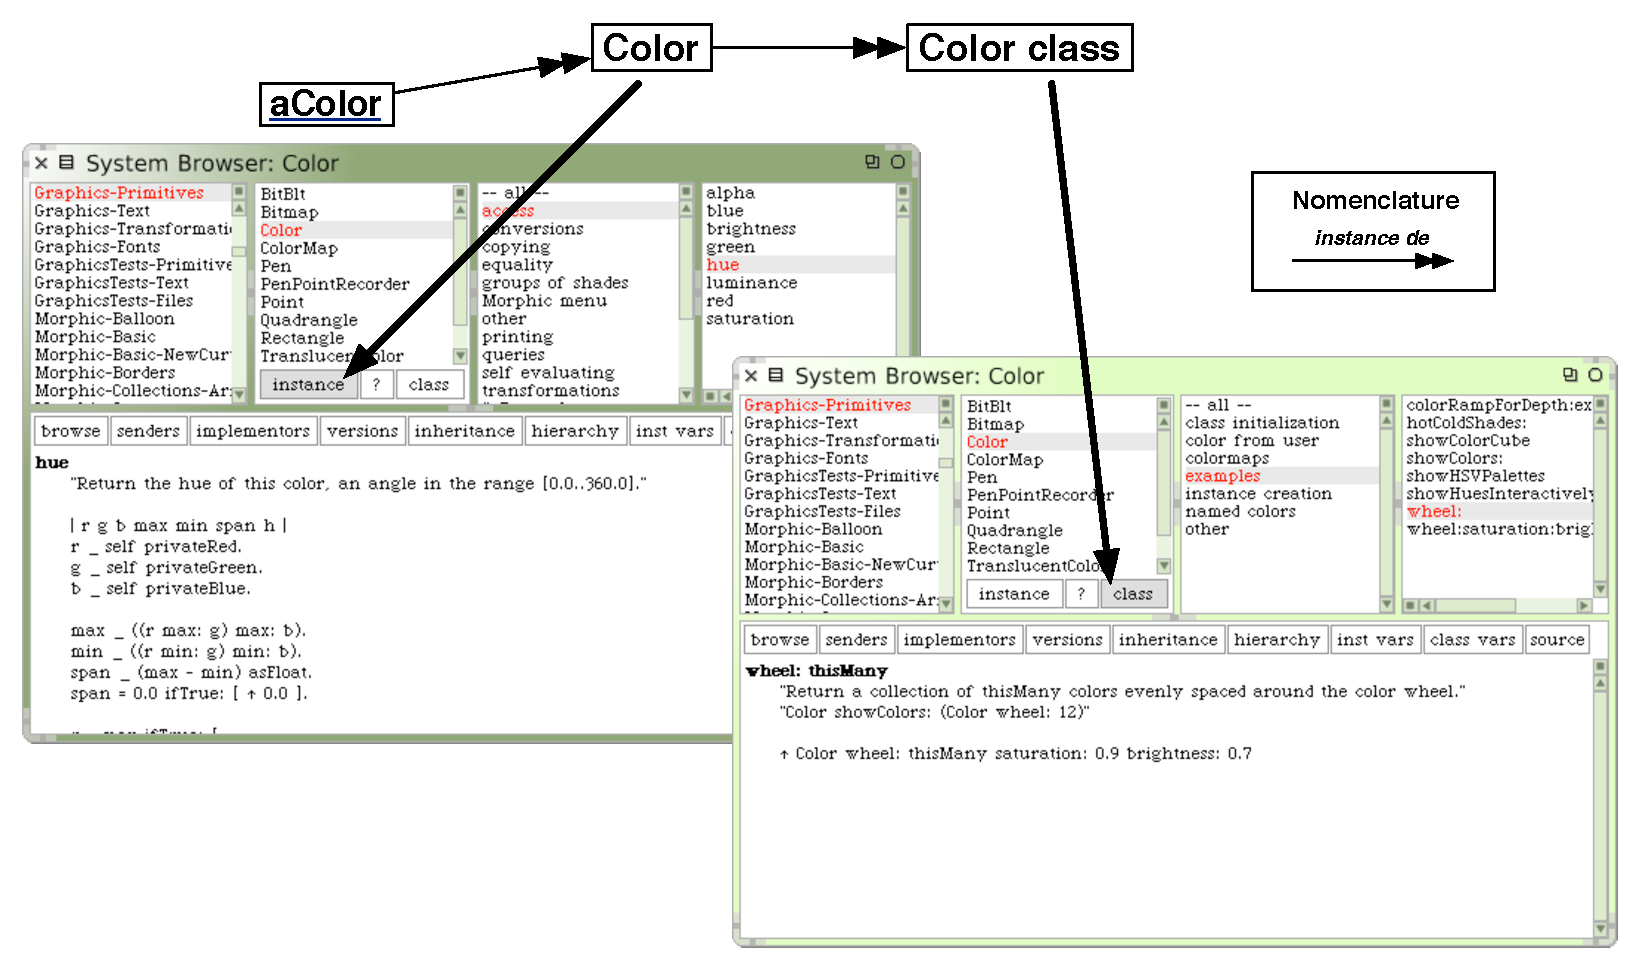
\includegraphics[width=\textwidth]{Color-Buttons}
\caption{Naviguer dans une classe et sa m\'eta-classe.
% \sd{Do we use Key everywhere in the picture as a legend indicator?}
% \on{sure, wherever appropriate}
\label{fig:Buttons}}
\end{center}
\end{figure}

De ce fait, le navigateur de classes nomm\'e \ind{System Browser} vous
aide \`a parcourir \`a la fois classes et m\'eta-classes comme si elles
n'\'etaient qu'une seule entit\'e avec deux ``c\^ot\'es'': le ``\subind{System Browser}{c\^ot\'e instance}'' et le ``\subind{System Browser}{c\^ot\'e classe}'', comme le montre la \figref{Buttons}. 
\damien{something wrong here. The text between quotes is not generated}
% true: \ind should replace \index there! (martial)
En cliquant sur le 
bouton \button{instance}, vous voyez la pr\'esentation de la classe \ct{Color}, \ie vous pouvez naviguer dans les m\'ethodes qui sont ex\'ecut\'ees quand
les messages sont envoy\'es \`a une instance de
\ct{Color}, comme la couleur blue (correspondant au bleu). En appuyant
sur le bouton \button{class} (pour classe), vous naviguez dans la classe \ct{Color class}, autrement dit vous voyez les m\'ethodes qui seront ex\'ecut\'ees
en envoyant les messages directement \`a la classe \ct{Color} elle-m\^eme.
Par exemple, \ct{Color blue} envoie le message \ct{blue} (pour \emph{bleu}) \`a
la classe \clsind{Color}.
Vous trouverez donc la m\'ethode \ct{blue} d\'efinie c\^ot\'e classe de la classe \ct{Color} et non du c\^ot\'e instance.
\seeindex{c\^ot\'e instance}{System Browser!c\^ot\'e instance}
\seeindex{c\^ot\'e classe}{System Browser!c\^ot\'e classe}
\seeindex{navigateur de classes!c\^ot\'e instance}{System Browser!c\^ot\'e instance}
\seeindex{navigateur de classes!c\^ot\'e classe}{System Browser!c\^ot\'e classe}


\needlines{5}
\begin{code}{@TEST | aColor |}
aColor := Color blue.               "!M\'ethode! de classe blue"
aColor        --> Color blue
aColor red  --> 0.0         "!M\'ethode d'acc\`es red (rouge) c\^ot\'e instance!"
aColor blue --> 1.0        "!M\'ethode d'acc\`es blue (bleu) c\^ot\'e instance!"
\end{code}

Vous d\'efinissez une classe en remplissant le patron (ou \emph{template} en anglais) propos\'e
dans le \subind{System Browser}{c\^ot\'e instance}.
Quand vous acceptez ce patron, le syst\`eme cr\'ee non seulement la classe
que vous d\'efinissez mais aussi la m\'eta-classe correspondante.
Vous pouvez naviguer dans la m\'eta-classe en cliquant sur le bouton \button{class}.
Du patron employ\'e pour la cr\'eation de la m\'eta-classe, seule la
liste des noms des variables d'instance vous est propos\'ee pour une \'edition directe.  

Une fois que vous avez cr\'e\'e une classe, cliquer sur
le bouton \button{instance} vous permet d'\'editer et de parcourir les
m\'ethodes qui seront poss\'ed\'ees par les instances de cette classe (et de ses sous-classes). Par exemple, nous pouvons voir dans la \figref{Buttons} que 
la m\'ethode \ct{hue} est d\'efinie pour les instances de la classe \ct{Color}.
A contrario, le bouton \button{class} vous laisse parcourir et \'editer
la m\'eta-classe (dans ce cas \ct{Color class}).

%---------------------------------------------------------
\subsection{Les m\'ethodes de classe} 

Les m\'ethodes de classe peuvent \^etre relativement utiles; naviguez dans \ct{Color class} pour voir quelques bons exemples.
Vous verrez qu'il y a deux sortes de \subind{classe}{m\'ethode}{s} d\'efinies dans une classe: celles qui cr\'eent les instances de la classe, comme \cmind{Color class}{blue} et celles qui ont une action \emph{utilitaire}, 
% martial: j'ai mis volontairement \emph pour l'adjectif utilitaire
comme \cmind{Color class}{showColorCube}.
Ceci est courant, bien que vous trouverez occasionnellement des m\'ethodes
de classe utilis\'ees d'une autre mani\`ere.

Il est coutumier de placer des m\'ethodes utilitaires dans le \subind{System Browser}{c\^ot\'e classe} parce qu'elles peuvent \^etre ex\'ecut\'ees
sans avoir \`a cr\'eer un objet additionnel dans un premier temps.
En fait, beaucoup d'entre elles contiennent un commentaire pour les rendre plus compr\'ehensible spour l'utilisateur qui les ex\'ecute.

\dothis{Naviguez dans la m\'ethode \ct{Color class>>>showColorCube}, double-cliquez \`a l'int\'erieur des guillements englobant le commentaire \ct{"Color showColorCube"} et tape au clavier \short{d}.}
Vous verrez l'effet de l'ex\'ecution de cette m\'ethode.  (S\'electionnez \menu{World \go \ind{restore display}~(r)} pour annuler les effets.)

Pour les familiers de \ind{Java} et \ind{C++},  les m\'ethodes de classe peuvent \^etre assimil\'ees aux m\'ethodes statiques. 
N\'eanmoins, l'homog\'en\'eit\'e de \st induit une diff\'erence:  les m\'ethodes statiques de Java sont des fonctions r\'esolues de mani\`ere statique alors que les m\'ethodes de classe de \st sont des m\'ethodes \`a transfert dynamique~\footnote{En anglais, dynamically-dispatched methods.} Ainsi, l'h\'eritage, la surcharge et l'utilisation de \emph{super} fonctionnent avec les m\'ethodes de classe dans \st, ce qui n'est pas le cas avec les m\'ethodes statiques en Java.  

%---------------------------------------------------------
\subsection{Les variables d'instance de classe}
Dans le cadre des variables d'instance ordinaires,
toutes les instances d'une classe partagent le m\^eme ensemble
de noms de variable et les instances de ses sous-classes h\'eritent
de ces noms; cependant, chaque instance poss\`ede son propre jeu de valeurs.
C'est exactement la m\^eme histoire avec les \subind{classe!variables d'instance}{variables d'instance de classe}: chaque classe a ses propres variables d'instance de classe priv\'ees.
Une sous-classe h\'eritera de ces  variables d'instance de classe, \emph{mais elle aura ses propres copies priv\'ees de ces variables}.
Aussi vrai que les objets ne partagent pas les variables d'instance, les classes et leurs sous-classes ne partagent pas les variables d'instance de classe.

Vous pouvez utiliser une variable d'instance de classe \ct{count}~\footnote{En fran\c{c}ais, compteur.} afin de suivre le nombre d'instances vous cr\'eez pour une classe donn\'ee.
Cependant, les sous-classes ont leur propre variable \ct{count}, 
les instances des sous-classes seront compt\'ees s\'epar\'ement.

\paragraph{Exemple: les variables d'instance de classe ne sont pas partag\'ees avec les sous-classes.}
Soient les classes \ct{Dog} et \ct{Hyena}~\footnote{En fran\c{c}ais, chien et hy\`ene.} telles que \ct{Hyena} h\'erite de la variable d'instance de classe \ct{count} de la classe \ct{Dog}.

%martial: si mauvaise coupe:
\newpage
\begin{classdef}[dog]{Cr\'eer Dog et Hyena}
Object subclass: #Dog
	instanceVariableNames: ''
	classVariableNames: ''
	poolDictionaries: ''
	category: 'SBE-CIV'

Dog class
	instanceVariableNames: 'count'

Dog subclass: #Hyena
	instanceVariableNames: ''
	classVariableNames: ''
	poolDictionaries: ''
	category: 'SBE-CIV'
\end{classdef}

Supposons que nous ayons des m\'ethodes de classe de \ct{Dog} pour initialiser sa variable \ct{count} \`a \ct{0} et pour incr\'ementer cette derni\`ere quand de nouvelles instances sont cr\'e\'ees:
\begin{method}[dogcount]{Comptabiliser les nouvelles instances de Dog via count}
Dog class>>>initialize
	super initialize.
	count := 0.

Dog class>>>new
	count := count +1.
	^ super new

Dog class>>>count
	^ count
\end{method}

Maintenant, \`a chaque fois que nous cr\'eons un nouveau \ct{Dog}, son compteur
count est incr\'ement\'e. Il en est de m\^eme pour toute nouvelle instance de \ct{Hyena}, mais elles sont compt\'ees s\'epar\'ement:
\begin{code}{}
Dog initialize.
Hyena initialize.
Dog count     --> 0
Hyena count --> 0
Dog new.
Dog count     --> 1
Dog new.
Dog count     --> 2
Hyena new.
Hyena count --> 1
\end{code}
% ON: In order to make this a test, I need the previous code to be part of the setup. Bleh.

Remarquons aussi que les variables d'instance de classe sont priv\'ees \`a la classe tout comme les variables d'instance sont priv\'ees \`a l'instance. 
Comme les classes et leurs instances sont des objets diff\'erents,
il en r\'esulte que:
\important{Une classe n'a pas acc\`es aux variables d'instance de ses propres instances.}
\important{Une instance d'une classe n'a pas acc\`es aux variables d'instance de classe de sa classe.}
C'est pour cette raison que les m\'ethodes d'initialisation d'instance doivent 
toujours \^etre d\'efinies dans le \subind{System Browser}{c\^ot\'e instance}\,---\,le \subind{System Browser}{c\^ot\'e classe} n'ayant pas acc\`es aux variables d'instance, il ne pourrait y avoir initiali\-sation!  
% 2007-11-05 correction errata SBE
Tout ce que peut faire la classe, c'est d'envoyer des messages d'\ind{initialisation} \`a des instances nouvellement cr\'e\'ees; ces messages pouvant bien s\^ur utiliser les m\'ethodes d'acc\`es.

De m\^eme, les instances ne peuvent acc\'eder aux variables d'instance de classe
que de mani\`ere indirecte en envoyant les messages d'acc\`es \`a leur classe.

\ind{Java} n'a rien d'\'equivalent aux variables d'instance de classe.  
Les variables statiques en Java et en \ind{C++} ont plut\^ot des similitudes 
avec les variables de classe de \st dont nous parlerons dans \secref{classVars}: toutes les sous-classes et leurs instances partagent la m\^eme variable statique.

\paragraph{Exemple: D\'efinir un Singleton.}
Le patron de conception~\footnote{En anglais, nous parlons de \emph{Design Patterns}.} nomm\'e \ind{Singleton}~\cite{Alpe98a} offre un exemple-type de l'usage de variables d'instance de classe et de m\'ethodes de classe.
Imaginez que nous souhaitons d'une part, cr\'eer une classe \ct{WebServer} et d'autre part, s'assurer qu'il n'a qu'une et une seule instance en faisant appel au patron Singleton.

En cliquant sur le bouton \button{instance} dans le navigateur de classe, nous d\'efinissons la classe \clsind{WebServer} comme suit (\clsref{singleton}).

\begin{classdef}[singleton]{Un classe Singleton}
Object subclass: #WebServer
	instanceVariableNames: 'sessions' 	
	classVariableNames: '' 	
	poolDictionaries: ''
	category: 'Web'
\end{classdef}

Ensuite, en cliquant sur le bouton \button{class}, nous pouvons ajouter une variable d'instance \ct{uniqueInstance} au \subind{System Browser}{c\^ot\'e classe}.

\begin{classdef}[webserver]{Le c\^ot\'e classe de la classe Singleton}
WebServer class 	
	instanceVariableNames: 'uniqueInstance'
\end{classdef}

Par cons\'equence, la classe \ct{WebServer} a d\'esormais un autre variable d'instance, en plus des variables h\'erit\'ees telles que \ct{superclass} et \ct{methodDict}.

Nous pouvons maintenant d\'efinir une \subind{classe}{m\'ethode} de classe que nous appellerons \ct{uniqueInstance} comme dans \tmthref{uniqueInstance}. 
Pour commencer, cette m\'ethode v\'erifie si \ct{uniqueInstance} a \'et\'e initialis\'ee ou non: dans ce dernier cas,
la m\'ethode cr\'ee une instance et l'assigne \`a la variable d'instance de classe \ct{uniqueInstance}.  
\emph{In fine}, la valeur de \ct{uniqueInstance} est retourn\'ee.
Puisque \ct{uniqueInstance} est une variable d'instance de classe, cette m\'ethode peut directement y acc\'eder.
    
\begin{method}[uniqueInstance]{uniqueInstance (c\^ot\'e classe)}
WebServer class>>>uniqueInstance
     uniqueInstance ifNil: [uniqueInstance := self new].
     ^ uniqueInstance
\end{method}

La premi\`ere fois que l'expression \ct{WebServer uniqueInstance} est ex\'ecut\'ee, une instance de la classe \ct{WebServer} sera cr\'e\'ee et affect\'ee \`a la variable \ct{uniqueInstance}. 
La seconde fois, l'instance pr\'ec\'edemment cr\'e\'ee sera retourn\'ee au lieu d'y avoir une nouvelle cr\'eation. 

Remarquons que la clause conditionnelle \`a l'int\'erieur du code de cr\'eation
de \tmthref{uniqueInstance} est \'ecrite \ct{self new} et non 
\mbox{\ct{WebServer new}.}
Quelle en-est la diff\'erence?   Comme la m\'ethode \ct{uniqueInstance} est d\'efinie dans \ct{WebServer class}, vous pouvez penser qu'elles sont identiques.    En fait, tant que personne ne cr\'ee une sous-classe de \ct{WebServer}, elles sont pareilles. Mais en supposant que \ct{ReliableWebServer} est une sous-classe de \ct{WebServer} et qu'elle h\'erite de la m\'ethode \ct{uniqueInstance},
nous devrions nous attendre \`a ce que \ct{ReliableWebServer uniqueInstance} r\'eponde un \lct{ReliableWebServer}. L'utilisation de \self assure que cela arrivera car il sera li\'e \`a la classe correspondante.
Du reste, notez que \ct{WebServer} et \ct{ReliableWebServer} ont chacune
leur propre variable d'instance de classe nomm\'ee \ct{uniqueInstance}.  Ces
deux variables ont, bien entendu, diff\'erentes valeurs.

%=========================================================
\section{Toute classe a une super-classe}

%\ruleref{inheritance}

Chaque classe en \st h\'erite de son comportement et de la description
de sa structure d'une unique \emphind{super-classe}.
Ceci est \'equivalent \`a dire que \st a un \ind{h\'eritage} simple.

\needlines{2}
\begin{code}{@TEST}
SmallInteger superclass --> Integer
Integer superclass          --> Number
Number superclass        --> Magnitude
Magnitude superclass    --> Object
Object superclass           --> ProtoObject
ProtoObject superclass  --> nil
\end{code}

Traditionnellement, la racine de la hi\'erarchie d'h\'eritage en \st est la classe \clsind{Object} (``Objet'' en anglais; puisque tout est un objet).
En \squeak, la racine est en fait une classe nomm\'ee \clsind{ProtoObject}, mais
normalement, vous n'aurez aucune attention \`a accorder \`a cette classe.
\ct{ProtoObject} encapsule le jeu de messages restreint que tout objet \emph{doit} avoir.  
N'importe comment, la plupart des classes h\'eritent de \ct{Object} qui, pour
sa part, d\'efinit beaucoup de messages suppl\'ementaires que presque tous les
objets devraient comprendre et auquels ils devraient pouvoir r\'epondre.
\`A moins que vous ayez une autre raison de faire autrement, vous devriez
normalement g\'en\'erer des classes d'application par l'h\'eritage
de la classe \ct{Object} ou d'une de ses sous-classes lors de la cr\'eation de classe.

\dothis{Une nouvelle classe est normalement cr\'e\'ee par l'envoi du message
\ct{subclass: instanceVariableNames: ...}
\`a une classe existante.
Il y a d'autres m\'ethodes pour cr\'eer des classes.
Veuillez jeter un coup d'\oe il au protocole \prot{Kernel-Classes \go Class \go subclass creation} pour voir desquelles il s'agit.}
\scatindex{Kernel-Classes}
\protindex{cr\'eation}

%There is no special syntax for creating abstract classes in \st.
%An abstract class is an ordinary class in which the implementation of some methods is deferred to a subclass.
%This is repeated in the next section

Bien que \squeak ne dispose pas d'h\'eritage multiple, il incorpore depuis la version 3.9 un m\'ecanisme appel\'e 
% martial: footnote ajoute
\emphind{trait}{}s~\footnote{Dans le sens de trait de caract\`eres, nous faisons allusion ainsi \`a la g\'en\'etique du comportement d'une m\'ethode.} 
pour partager le comportement entre des classes distincts.
Les \emph{traits} sont des collections de m\'ethodes qui peuvent \^etre r\'eutilis\'ees par plusieurs classes sans lien d'h\'eritage. Employer les \emph{traits} vous permet de partager du code entre les diff\'erentes classes sans reproduire ce code.

%---------------------------------------------------------
\subsection{Les m\'ethodes abstraites et les classes abstraites}

Une classe \subind{classe}{abstraite} est une classe qui n'existe que pour \^etre h\'erit\'ee, au lieu d'\^etre instanci\'ee.
Une classe abstraite est habituellement incompl\`ete, dans le sens qu'elle ne d\'efinit pas toutes les m\'ethodes qu'elle utilise.
Les m\'ethodes ``manquantes''\,---\,celle que les autres m\'ethodes envoyent, mais qui ne sont pas d\'efinies elles-m\^eme\,---\,sont dites m\'e\-tho\-des \subind{m\'ethode}{abstraite}{s}.
\seeindex{classe abstraite}{classe, abstraite}
\seeindex{m\'ethode abstraite}{m\'ethode, abstraite}

\st n'a pas de syntaxe d\'edi\'ee pour dire qu'une m\'ethode ou qu'une classe est abstraite. 
Par convention, le corps d'une m\'ethode abstraite contient l'expression \ct{self subclassResponsibility}~\footnote{Dans le sens, laiss\'ee \`a la responsabilit\'e de la sous-classe.}. 
Ceci est connu sous le nom de ``marker method'' ou marqueur de m\'ethode; il indique que les sous-classes ont la responsabilit\'e de d\'efinir une version concr\`ete de la m\'ethode. 
Les m\'ethodes \ct{self subclassResponsibility} devraient toujours \^etre surcharg\'ees, et ainsi, ne devraient jamais \^etre ex\'ecut\'ees.
Si vous oubliez d'en surcharger une et que celle-ci est ex\'ecut\'ee, une exception sera lev\'ee. 
\cmindex{Object}{subclassResponsibility}

Une classe est consid\'er\'ee comme abstraite si une de ses m\'ethodes est abstraite.
Rien ne vous emp\^eche de cr\'eer une instance d'une classe abstraite; tout fonctionnera jusqu'\`a ce qu'une m\'ethode abstraite soit invoqu\'ee. 

\subsubsection{Exemple: la classe \ct{Magnitude}.}
\clsind{Magnitude} est une classe abstraite qui nous aide \`a d\'efinir
des objets pouvant \^etre comparables les uns avec les autres. Les
sous-classes de \ct{Magnitude} devraient impl\'ementer les m\'ethodes
\ct{<}, \ct{=} et \ct{hash}~\footnote{Relatif au code de hachage.}.
Gr\^ace \`a ces messages, \ct{Magnitude} d\'efinit d'autres m\'ethodes telles que
\ct{>}, \ct{>=}, \ct{<=}, \ct{max:}, \ct{min:} \ct{between:and:} et
d'autres encore pour comparer des objets.
Ces m\'ethodes sont h\'erit\'ees par les sous-classes.
La m\'ethode \mthind{Magnitude}{<} est abstraite et est d\'efinie comme
dans \tmthref{MagnitudeLessThan}.

\begin{method}[MagnitudeLessThan]{\ct{Magnitude>>><}. Le commentaire dit: ``r\'epond si le receveur est inf\'erieur \`a l'argument''.}
Magnitude>>>< aMagnitude 
	"Answer whether the receiver is less than the argument."
	^self subclassResponsibility
\end{method}

\noindent
A contrario, la m\'ethode \mthind{Magnitude}{>=} est concr\`ete; elle est d\'efinie en fonction de \ct{<}:

\begin{method}[Magnitude>=]{\ct{Magnitude>>>>=}. Le commentaire dit: ``r\'epond si le receveur est plus grand ou \'egal \`a l'argument''.}
>= aMagnitude 
	"Answer whether the receiver is greater than or equal to the argument."
	^(self < aMagnitude) not
\end{method}
Il en va de m\^eme des autres m\'ethodes de comparaison.

\clsind{Character} est une sous-classe de \ct{Magnitude}; elle surcharge la m\'ethode \mthind{Object}{subclassResponsibility} de \ct{<} avec sa propre version de \ct{<} (voir \mthref{CharacterLessThan}).  \ct{Character} d\'efinit aussi les m\'ethodes \ct{=} et \ct{hash}; elles h\'eritent les m\'ethodes \ct{>=}, \ct{<=}, \ct{~=} et autres de la classe \ct{Magnitude}.

\begin{method}[CharacterLessThan]{\ct{Character>>><}. Le commentaire dit: ``r\'epond vrai si la valeur du receveur est inf\'erieure \`a la valeur du l'argument''.}
Character>>>< aCharacter 
	"Answer true if the receiver's value < aCharacter's value."
	^self asciiValue < aCharacter asciiValue
\end{method}

%---------------------------------------------------------
\subsection{Traits}
Un \emphind{trait} est une collection de m\'ethodes qui peut \^etre incluse dans le comportement d'une classe sans le besoin d'un h\'eritage.
Les classes disposent non seulement d'une seule super-classe mais aussi de la facilit\'e offerte par le partage de m\'ethodes utiles avec d'autres m\'ethodes sans lien de parent\'e vis-\`a-vis de l'h\'eritage.

D\'efinir un nouveau \emph{trait} se fait en rempla\c{c}ant simplement le patron
pour la cr\'eation de la sous-classe par un message \`a la classe \clsind{Trait}.

\needspace{5\baselineskip}
\begin{classdef}[tauthor]{D\'efinir un nouveau \emph{trait}}
Trait named: #TAuthor
	uses: { }
	category: 'SBE-Quinto'
\end{classdef}

\noindent
Nous d\'efinissons ici le \emph{trait} \ct{TAuthor} dans la cat\'egorie \scat{SBE-Quinto}.
Ce \emph{trait} n'\emph{utilise}~\footnote{Terme anglais: \emph{uses}: il signifie ``utilise''.} aucun autre \emph{trait} existant.
En g\'en\'eral, nous pouvons sp\'ecifier l'\emph{expression de composition d'un trait} par d'autres \emph{traits} en u\-ti\-li\-sant le mot-cl\'e \ct{uses:}.
Dans notre cas, nous \'ecrivons un tableau vide \mbox{(\{ \}).}

Les \emph{traits} peuvent contenir des m\'ethodes, mais aucune variable d'instance.
Supposons que nous voulons ajouter une m\'ethode \ct{author} (auteur en anglais) \`a diff\'erentes classes sans lien hi\'erarchique;
nous le ferions ainsi:

\begin{method}[author]{D\'efinir la m\'ethode author}
TAuthor>>>author
    "Returns author initials"
	^ 'on'    "oscar nierstrasz"
\end{method}

\noindent
Maintenant nous pouvons employer ce \emph{trait} dans une classe ayant d\'ej\`a sa propre super-classe, disons, la classe \ct{SBEGame} que nous avons d\'efinie dans \charef{firstApp}.
Nous n'avons qu'\`a modifier le patron de cr\'eation de la classe \ct{SBEGame} pour y inclure cette fois l'argument-cl\'e \ct{uses:} suivi du \emph{trait} \`a utiliser: \ct{TAuthor}.

\begin{classdef}[sbegamewithtrait]{Utiliser un trait}
BorderedMorph subclass: #SBEGame
	uses: TAuthor
	instanceVariableNames: 'cells'
	classVariableNames: ''
	poolDictionaries: ''
	category: 'SBE-Quinto'
\end{classdef}

Si nous instantions maintenant \ct{SBEGame}, l'instance r\'epondra comme pr\'evu au message \ct{author}.

\begin{code}{}
SBEGame new author --> 'on'
\end{code}

Les expressions de composition de \emph{trait} peuvent combiner plusieurs \emph{traits} via l'op\'erateur \ct{+}.
En cas de conflit (\ie quand plusieurs \emph{traits} d\'efinissent des m\'ethodes avec le m\^eme nom), ces conflits peuvent \^etre r\'esolus en retirant explicitement ces m\'ethodes (avec \ct{-}) ou en red\'efinissant ces m\'ethodes dans la classe ou le \emph{trait} que vous \^etes en train de d\'efinir.
Il est possible aussi de cr\'eer un \emph{alias} des m\'ethodes (avec \ct{@}) 
leur fournissant ainsi un nouveau nom.

Les \emph{traits} sont employ\'es dans le noyau du syst\`eme~\footnote{En anglais, System kernel.}.
Un bon exemple est la classe \clsind{Behavior}.

\needlines{8}
\begin{classdef}[behaviorwithtraits]{Behavior d\'efinit par les \emph{traits}}
Object subclass: #Behavior
	uses: TPureBehavior @ {#basicAddTraitSelector:withMethod:->#addTraitSelector:withMethod:}
	instanceVariableNames: 'superclass methodDict format'
	classVariableNames: 'ObsoleteSubclasses'
	poolDictionaries: ''
	category: 'Kernel-Classes'
\end{classdef}
\noindent
Ici, nous voyons que la m\'ethode \ct{basicAddTraitSelector:withMethod:} d\'efinie dans le \emph{trait} \ct{TPureBehavior} a \'et\'e renomm\'ee en \mbox{\ct{addTraitSelector:withMethod:}.}
%-Here we see that the method \ct{addTraitSelector:withMethod:} defined in the trait \ct{TPureBehavior} has been aliased to \ct{basicAddTraitSelector:withMethod:}.
Les \emph{traits} sont \`a pr\'esent support\'es par les navigateurs de classe (ou \emph{browsers}).

%=========================================================
\section{Tout se passe par envoi de messages}

%\ruleref{message}

Cette r\`egle r\'esume l'essence m\^eme de la programmation en \st.

Dans la programmation proc\'edurale, lorsqu'une proc\'edure est appel\'ee, l'appelant (\emph{caller}, en anglais) fait le choix du morceau de code \`a ex\'ecuter; il choisit la proc\'edure ou la fonction \`a ex\'ecuter \emph{statiquement}, par nom.  

En programmation orient\'ee objet, nous ne faisons \emph{pas} d'``appel de m\'ethodes''. Nous faisons un ``\subind{message}{envoi} de messages.''
Le choix de terminologique est important.
Chaque objet a ses propres responsabilit\'es.
Nous ne pouvons \emph{dire} \`a un objet ce qu'il faut faire en lui imposant 
une proc\'edure.
Au lieu de cela, nous devons lui \emph{demander} poliment de faire quelque chose en lui envoyant un message.
Le message n'est \emph{pas} un morceau de code: ce n'est rien d'autre qu'un nom (s\'electeur) et une liste d'arguments.
Le receveur d\'ecide alors de comment y r\'epondre en s\'electionnant en retour
sa propre m\'ethode correspondant \`a ce qui a \'et\'e demand\'e.
Puisque des objets distincts peuvent avoir diff\'erentes m\'ethodes pour r\'epondre \`a un m\^eme message, le choix de la m\'ethode doit se faire \emph{dynamiquement} \`a la r\'eception du message.
\begin{code}{@TEST}
3 + 4         --> 7          "!envoie le message + d'argument 4 \`a l'entier  3!"
(1@2) + 4 --> 5@6    "envoie le message + d'argument 4 au point (1@2)"
\end{code}
\noindent
En cons\'equence, nous pouvons envoyer le \emph{m\^eme message} \`a diff\'erents objets, chacun pouvant avoir \emph{sa propre m\'ethode} en r\'eponse au message.
Nous ne disons pas \`a \ct{SmallInteger} \ct{3} ou au \ct{Point} \ct{1@2} comment r\'epondre au message \ct{+ 4}.
Chacun a sa propre m\'ethode pour r\'epondre \`a cet envoi de message, et r\'epond ainsi selon le cas.

L'une des cons\'equences du mod\`ele de transmission de message de \st est qu'il encourage un style de programmation dans lequel les objets tendent \`a avoir des m\'ethodes tr\`es compactes en d\'el\'eguant des t\^aches aux autres objets, plut\^ot que d'impl\'ementer de gigantesques m\'ethodes proc\'edurales engendrant trop de responsabilit\'e.
Joseph Pelrine
\ab{Citation?}
\on{d\'esol\'e, simple communiqu\'e personel de l'auteur et notes de lecture!}
dit succintement le principe suivant:
\important{Ne fais rien que tu ne peux d\'el\'eguer \`a quelqu'un d'autre~\traduit{Don't do anything that you can push off onto someone else.}.}
\index{Pelrine, Joseph}

Beaucoup de langages orient\'es objets disposent \`a la fois d'op\'erations statiques et dynamiques pour les objets; en \st il n'y a qu'envois de messages dynamiques. Au lieu de fournir des op\'erations statiques sur les classes, nous leur envoyons simplement des messages, puisque les classes sont aussi des objets. 

\emph{Pratiquement} tout en \st se passe par envoi de messages.
\`A certains stades, le pragmatisme doit prendre le relais:
\begin{itemize}
  \item Les \emph{d\'eclarations de variable} ne reposent pas sur l'envoi de message.
  		En fait, les \subind{variable}{d\'eclaration}{}s de variable ne sont m\^eme pas ex\'ecutables.
  		D\'eclarer une variable produit simplement l'allocation d'un espace pour la r\'ef\'erence de l'objet.
  \item Les \emph{affectations} (ou assignations) ne reposent pas sur l'envoi de message.
  		L'\ind{affectation} d'une variable produit une liaison de nom de variable dans le cadre de sa d\'efinition.
  \item Les \emph{retours} (ou renvois) ne reposent pas sur l'envoi de message.
  		Un \ind{retour} ne produit que le retour \`a l'envoyeur du r\'esultat calcul\'e.
  \item Les \emph{primitives} ne reposent pas sur l'envoi de message.
  		Elles sont cod\'ees au niveau de la \ind{machine virtuelle}.
		\index{primitive}
\end{itemize}

\`A quelques autres exceptions pr\`es, presque tout le reste se d\'eroule v\'eritablement par l'envoi de messages. 
En particulier, la seule fa\c{c}on de mettre \`a jour une \ind{variable d'instance} d'un autre objet est de lui envoyer un message r\'eclamant le changement de son propre attribut (ou champ) car ces derniers ne sont pas des ``attributs publics'' en \st.
Bien entendu, offrir des m\'ethodes d'acc\`es dites accesseurs (\emph{getter}, en anglais, retournant l'\'etat de la variable) et mutateurs (\emph{setter} en anglais, changeant la variable) pour chaque variable d'instance d'un objet n'est pas une bonne m\'ethodologie orient\'ee objet.
Joseph Pelrine annonce aussi \`a juste titre:
\important{Ne laissez jamais personne d'autre jouer avec vos donn\'ees~\traduit{Don't let anyone else play with your data.}.}

%=========================================================
\section{La recherche de m\'ethode suit la cha\^{\i}ne d'h\'eritage} 

%\ruleref{lookup}

Qu'arrive-t-il exactement quand un objet re\c{c}oit un message?

Le processus est relativement simple:
la classe du receveur cherche la m\'ethode \`a utiliser pour
op\'erer le message.
Si cette classe n'a pas de m\'ethode, elle demande \`a sa \ind{super-classe} et remonte ainsi de suite la cha\^{\i}ne d'\ind{h\'eritage}.
Quand la m\'ethode est enfin trouv\'ee, les arguments sont affect\'es aux param\`etres de la m\'ethode et la \ind{machine virtuelle} l'ex\'ecute.
\index{m\'ethode!lookup}
\index{m\'ethode!r\'eferencement}

C'est, en essence, aussi simple que cela.
Mais il reste quelques questions auxquelles nous devons prendre soin de r\'epondre:

\begin{itemize}
  \item \emph{Que se passe-t-il lorsque une m\'ethode ne renvoie pas explicitement une valeur?}
  \item \emph{Que se passe-t-il quand une classe r\'eimpl\'emente une m\'ethode d'une super-classe?}
  \item \emph{Qu'elle diff\'erence y a-t-il entre les envois faits \`a \pvind{self} et ceux faits \`a \pvind{super}?}
  \item \emph{Que se passe-t-il lorsqu'aucune m\'ethode est trouv\'ee?}
\end{itemize}

Les r\`egles pour la recherche par r\'ef\'erencement (en anglais \emph{lookup}) pr\'esent\'ees ici sont conceptuelles: des r\'ealisations au sein de la machine virtuelle rusent pour optimiser la vitesse de recherche des m\'ethodes. 
C'est leur travail mais tout est fait pour que vous ne remarqueriez jamais qu'elles font quelque chose de diff\'erent des r\`egles \'enonc\'ees.
% Whatever the implementation does, these rules will give you a clear understanding of the semantics of sending messages to \self and \super.

Tout d'abord, penchons-nous sur la strat\'egie de base de la recherche. Ensuite
nous r\'epondrons aux questions.

%---------------------------------------------------------
\subsection{La recherche de m\'ethode}
Supposons la cr\'eation d'une instance de \ct{EllipseMorph}.
\begin{code}{@TEST | anEllipse |}
anEllipse := EllipseMorph new.
\end{code}
\noindent
Si nous envoyons \`a cet objet le message \ct{defaultColor}, nous obtenons le r\'esultat \ct{Color yellow}~\footnote{Yellow est la couleur jaune.}:
\begin{code}{@TEST | anEllipse | anEllipse := EllipseMorph new.}
anEllipse defaultColor --> Color yellow
\end{code}
\noindent
La classe \ct{EllipseMorph} impl\'emente \ct{defaultColor}, donc la m\'ethode ad\'equate est trouv\'ee imm\'ediatement.

\begin{method}[defaultColor]{Une m\'ethode impl\'ement\'ee localement. Le commentaire dit: ``retourne la couleur par d\'efaut; le style de remplissage pour le receveur''.}
EllipseMorph>>>defaultColor
	"answer the default color/fill style for the receiver"
	^ Color yellow
\end{method}
\cmindex{EllipseMorph}{defaultColor}

A contrario, si nous transmettons le message \ct{openInWorld} \`a \mbox{\ct{anEllipse},} la m\'ethode n'est pas trouv\'ee imm\'ediatement parce que la classe \ct{EllipseMorph} n'impl\'emente pas \ct{openInWorld}.
La recherche continue plus avant dans la super-classe \mbox{\lct{BorderedMorph},} puis ainsi de suite, jusqu'\`a ce qu'une m\'ethode \ct{openInWorld} soit trouv\'ee dans la classe \ct{Morph} (voir \figref{openInWorldLookup}).

\begin{method}[openInWorld]{Une m\'ethode h\'erit\'ee. Le commentaire dit: ``Ajoute ce morph dans le monde (world). Si le mode MVC est actif alors lui fournir une fen\^etre Morphic.''.}
Morph>>>openInWorld
	"Add this morph to the world.  If in MVC, then provide a Morphic window for it."
	self couldOpenInMorphic
		ifTrue: [self openInWorld: self currentWorld]
		ifFalse: [self openInMVC]
\end{method}
\cmindex{Morph}{openInWorld}

\begin{figure}[htb]
\begin{center}
\ifluluelse
	{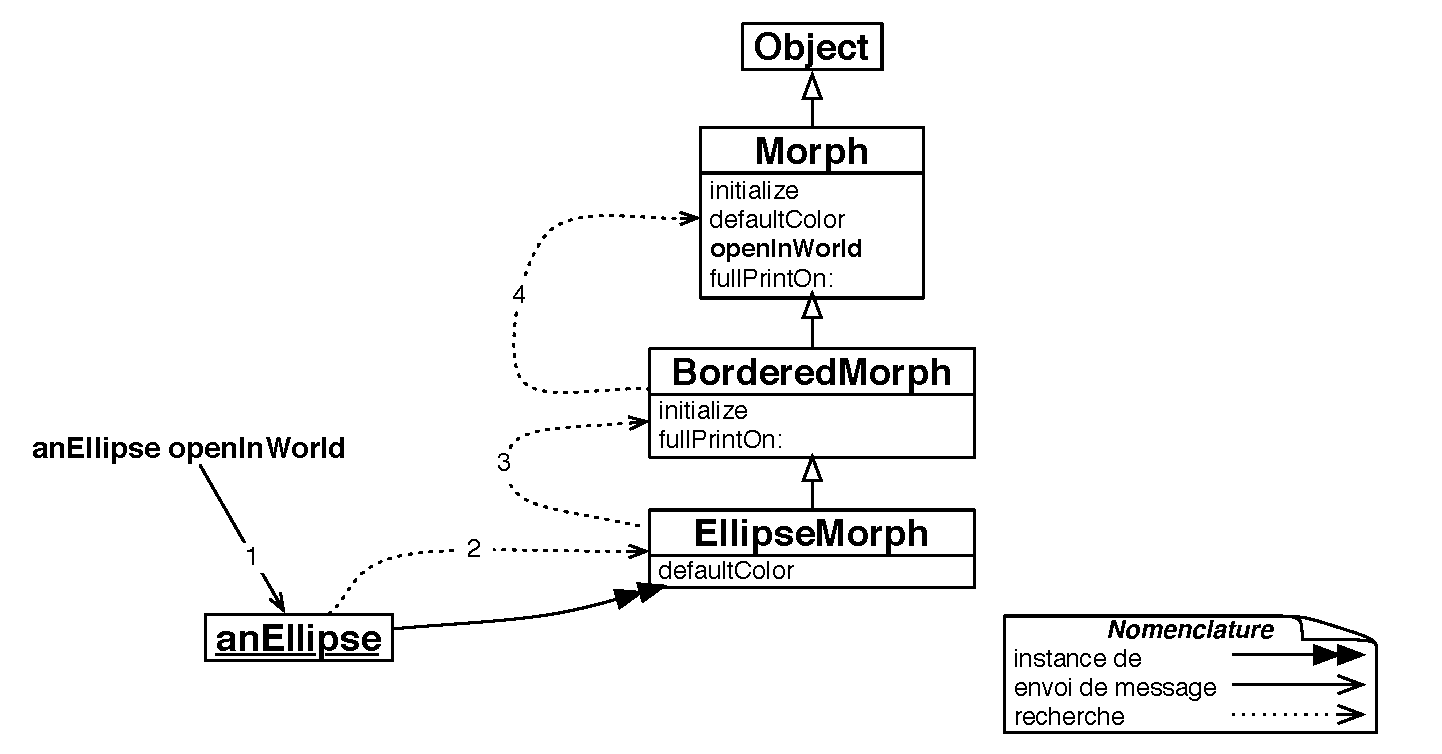
\includegraphics[width=\textwidth]{openInWorldLookup}}
	{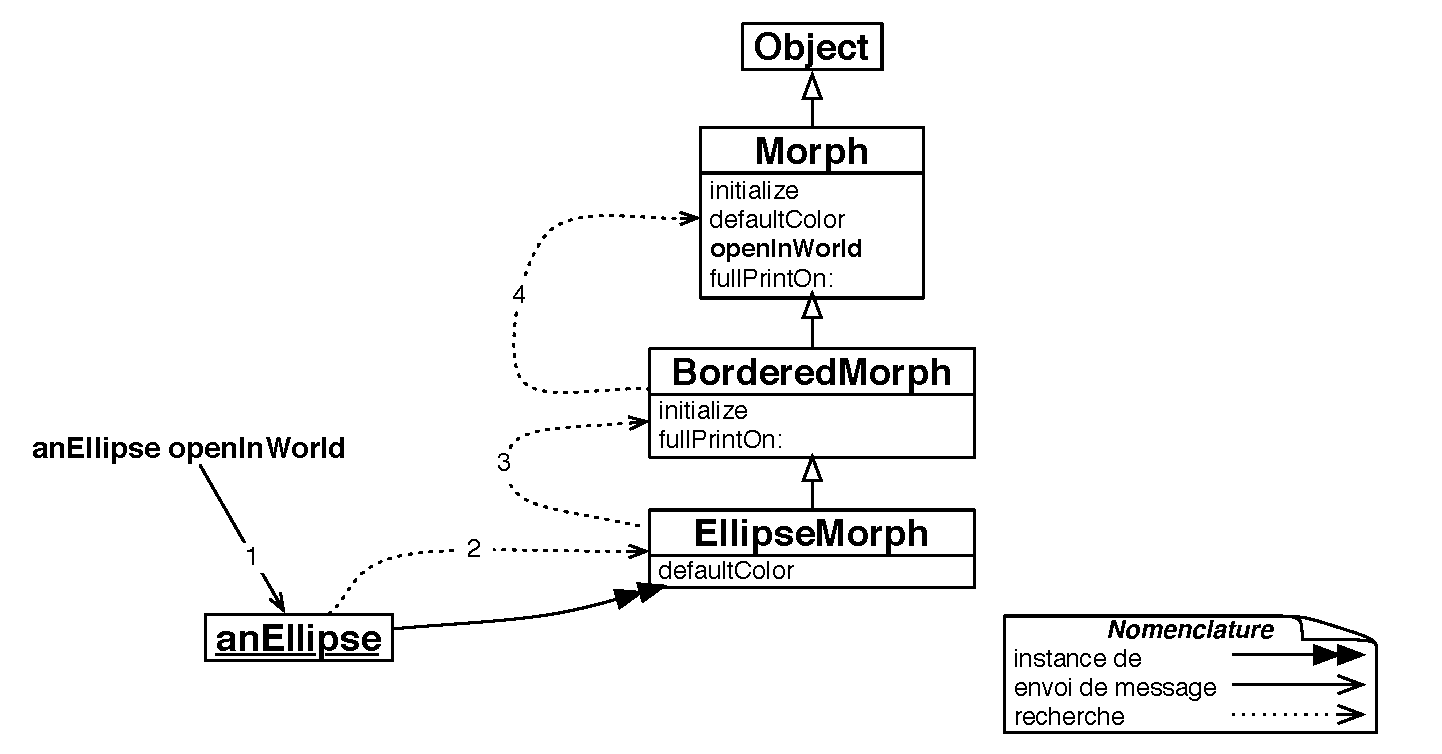
\includegraphics[width=0.8\textwidth]{openInWorldLookup}}
\caption{Recherche par r\'ef\'erencement d'une m\'ethode suivant la hi\'erarchie d'h\'eritage.\label{fig:openInWorldLookup}}
\end{center}
\end{figure}

%---------------------------------------------------------
\subsection{Renvoyer self}

Remarquez que \ct{EllipseMorph>>>defaultColor} (\mthref{defaultColor}) renvoie explicitement \ct{Color yellow} alors que \ct{Morph>>>openInWorld} (\mthref{openInWorld}) semble ne rien retourner.

En r\'ealit\'e une m\'ethode renvoie \emph{toujours} un message avec une valeur\,---\,qui est, bien entendu, un objet.
La r\'eponse peut \^etre d\'efinit par la construction en \ct{^} dans la m\'ethode, mais si l'ex\'ecution atteint la fin de la m\'ethode sans ex\'ecuter un \ct{^}, la m\'ethode retournera toujours une valeur: l'objet receveur lui-m\^eme.
Nous disons habituellement que la m\'ethode ``renvoie \self'', parce qu'en
\st la pseudo-variable \self repr\'esente le receveur du message. En \ind{Java}, nous utilisons \ct{this}.
\index{variable!pseudo}
%\index{return}
\index{renvoi}
\index{retour}
\seeindex{caret}{renvoi}
\seeindex{caret}{retour}

Ceci induit le constat suivant: \tmthref{openInWorld} est \'equivalent \`a \mbox{\tmthref{openInWorldReturnSelf}:}

\needlines{5}
\begin{method}[openInWorldReturnSelf]{Renvoi explicite de \mbox{\self.} Le dernier commentaire dit: ``Ne faites pas cela \`a moins d'en \^etre s\^ur''.}
Morph>>>openInWorld
	"Add this morph to the world.  If in MVC,
	then provide a Morphic window for it."
	self couldOpenInMorphic
		ifTrue: [self openInWorld: self currentWorld]
		ifFalse: [self openInMVC].
	^ self		"Don't do this unless you mean it!"
\end{method}

Pourquoi \'ecrire \ct{^ self} explicitement n'est pas une bonne chose \`a faire?
Parce que, quand vous renvoyez explicitement quelque chose, vous communiquez
que vous retournez quelque chose d'importance \`a l'exp\'editeur du message.
D\`es lors vous sp\'ecifiez que vous attendez que l'exp\'editeur fasse quelque chose de la valeur retourn\'ee.
Puisque ce n'est pas le cas ici, il est pr\'ef\'erable de ne pas renvoyer explicitement \self.

C'est une convention en \st, ainsi r\'esum\'e par Kent Beck se r\'ef\'erant \`a la \emph{valeur de retour importante} ``Interesting return value'' \cite{Beck97a}:
\index{Beck, Kent}

\important{Renvoyez une valeur seulement quand votre objet exp\'editeur en a l'usage~\traduit{Return a value only when you intend for the sender to use the value.}.}

%---------------------------------------------------------
\subsection{Surcharge et extension.}

Si nous revenons \`a la hi\'erarchie de classe \ct{EllipseMorph} dans \figref{openInWorldLookup}, nous voyons que les classes \ct{Morph} et \mbox{\ct{EllipseMorph}} impl\'ementent toutes deux \ct{defaultColor}.
En fait, si nous ouvrons un nouvel \'el\'ement graphique \emph{morph} (\ct{Morph new openInWorld}), nous constatons que nous obtenons un morph bleu, l\`a o\`u l'ellipse (\ct{EllipseMorph}) est jaune (yellow) par d\'efaut.
\index{m\'ethode!surcharge}
\index{m\'ethode!extension}
\seeindex{surcharge}{m\'ethode, surcharge}
\seeindex{extension}{m\'ethode, extension}

Nous disons que \ct{EllipseMorph} \emph{surcharge} la m\'ethode \ct{defaultColor} qui h\'erite de \ct{Morph}.
La m\'ethode h\'erit\'ee n'existe plus du point de vue \ct{anEllipse}.

Parfois nous ne voulons pas surcharger les m\'ethodes h\'erit\'ees, mais plut\^ot les \emph{\'etendre} avec de nouvelles fonctionnalit\'es; autrement dit, nous souhaiterions pouvoir invoquer la m\'ethode surcharg\'ee \emph{compl\'et\'ee} par la nouvelle fonctionnalit\'e que nous aurons d\'efinie dans la sous-classe.
En \st, comme dans beaucoup de langages orient\'es objet reposant sur l'h\'eritage simple, nous pouvons le faire \`a l'aide d'un envoi de message \`a \super.

La m\'ethode \ct{initialize} est l'exemple le plus important de l'application de ce m\'ecanisme.
Quand une nouvelle instance d'une classe est initialis\'ee, il est vital
d'initialiser toutes les variables d'instance h\'erit\'ees.
Cependant, les m\'ethodes \ct{initialize} de chacune des super-classes
de la cha\^{\i}ne d'h\'eritage fournissent d\'ej\`a la connaissance
n\'ecessaire. 
La sous-classe n'a pas \`a s'occuper d'initialiser les variables d'instance h\'erit\'ees!

C'est une bonne pratique d'envoyer \ct{super initialize} avant tout autre consid\'eration lorsque nous cr\'eons une m\'ethode d'\ind{initialisation}:
\index{super!initialize}

\needlines{6}
\begin{method}[morphinit]{Super initialize. Le commentaire dit: ``initialise l'\'etat du receveur''.}
BorderedMorph>>>initialize
	"initialize the state of the receiver"
	super initialize.
	self borderInitialize
\end{method}

\important{Une m\'ethode \ct{initialize} devrait toujours commencer par la ligne \ct{super initialize}.}

%---------------------------------------------------------
\subsection{Self et super}

Nous avons besoin des \subind{super}{transmission}{}s sur \super pour 
r\'eutiliser le comportement h\'erit\'e qui pourrait sinon \^etre
surcharg\'e.
Cependant, la technique habituelle de composition de m\'ethodes,
h\'erit\'ees ou non, est bas\'ee sur la \subind{self}{transmission} sur
\self.

Comment la transmission sur \self diff\`ere de celle avec \super?
Comme \self, \super repr\'esente le receveur du message.
La seule diff\'erence est dans la \subind{recherche}{m\'ethode} de recherche.
Au lieu de faire partir la recherche depuis la classe du receveur,
celle-ci d\'emarre dans la super-classe de la m\'ethode dans laquelle la
transmission sur \super se produit. 

Remarquez que \super n'est \emph{pas} la super-classe!
C'est une erreur courante et normale que de le penser.
C'est aussi une erreur de penser que la recherche commence dans la super-classe du receveur.
Nous allons voir pr\'ecisemment comment cela marche avec l'exemple suivant.

Consid\'erons le message \ct{initString}, que nous pouvons envoyer \`a 
n'importe quel morph:
\begin{code}{@TEST | anEllipse | anEllipse := EllipseMorph new.}
anEllipse initString --> '(EllipseMorph newBounds: (0@0 corner: 50@40) color: Color yellow) setBorderWidth: 1 borderColor: Color black'
\end{code}
La valeur de retour est une cha\^{\i}ne de caract\`eres qui peut \^etre
\'evalu\'ee pour recr\'eer un morph.

Comment ce r\'esultat est-il exactement obtenu gr\^ace \`a l'association
de \self et de \super?
Pour commencer, 
\ct{anEllipse initString} trouvera la m\'ethode \ct{initString} dans la 
classe \ct{Morph},
comme vu dans \figref{initStringLookup}.

\begin{figure}[htb]
\begin{center}
\ifluluelse
	{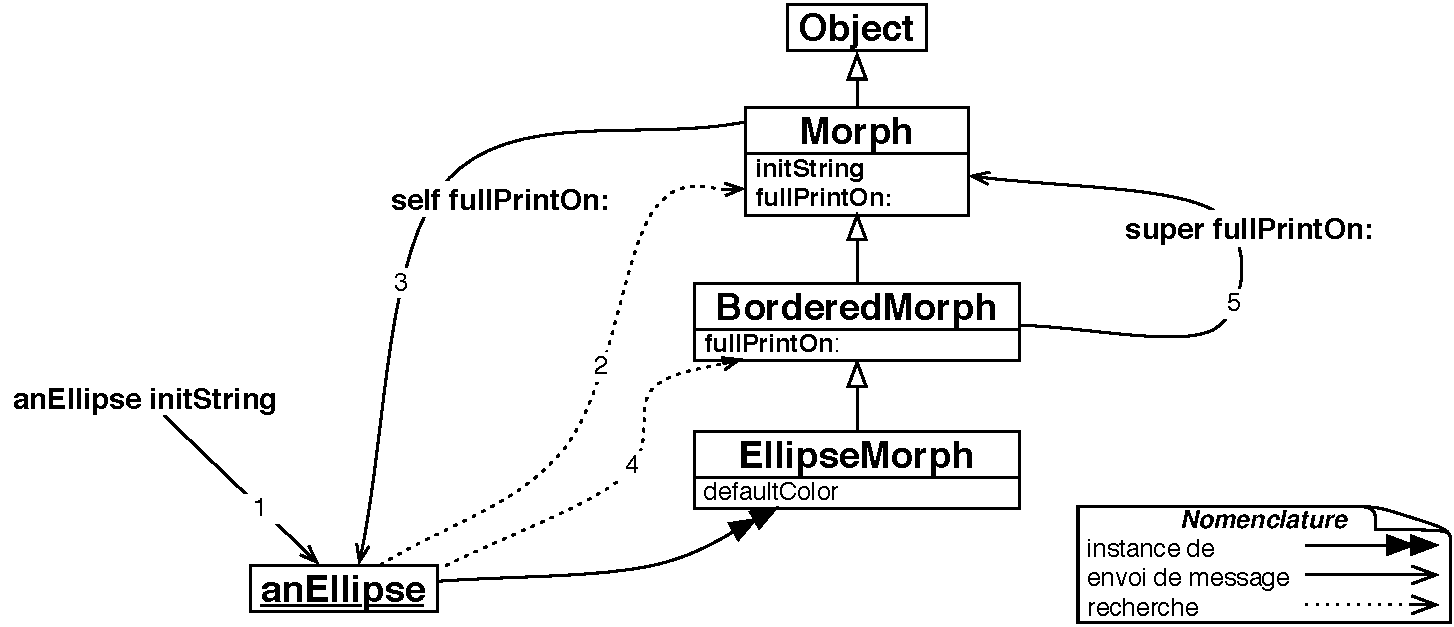
\includegraphics[width=\textwidth]{initStringLookup}}
	{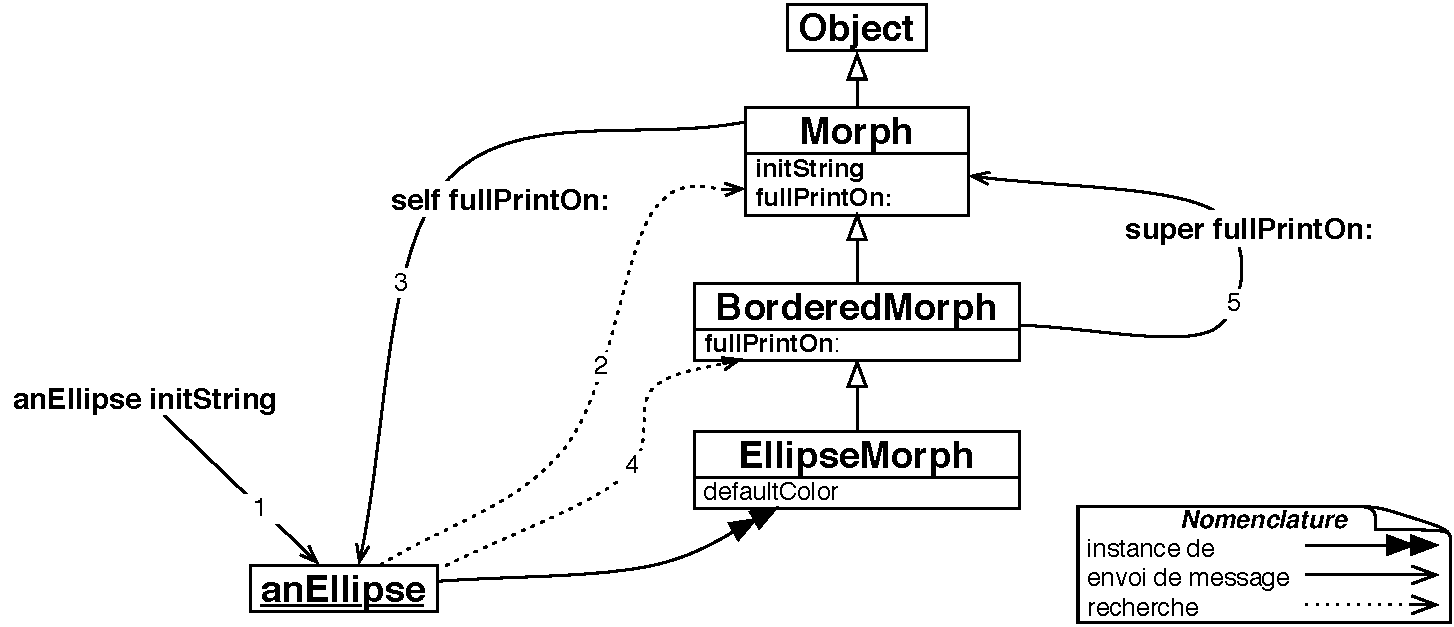
\includegraphics[width=0.8\textwidth]{initStringLookup}}
\caption{Les transmissions sur \self et \super.\label{fig:initStringLookup}}
\end{center}
\end{figure}

\needlines{5}
\begin{method}[initString]{Une transmission sur \self}
Morph>>>initString
	^ String streamContents: [:s | self fullPrintOn: s]
\end{method}
La m\'ethode \cmind{Morph}{initString} envoie \ct{fullPrintOn:} \`a \self,
ce qui entra\^{\i}ne une seconde recherche, d\'emarrant dans la classe
\ct{EllipseMorph}, trouvant \mthind{BorderedMorph}{fullPrintOn:} dans \ct{BorderedMorph} (voir \figref{initStringLookup} encore une fois).
Ce qu'il faut noter, c'est que la transmission sur \self
fait d\'emarrer encore la recherche de m\'ethode dans la classe du 
receveur, \ie la classe de
\ct{anEllipse}.

\important{Une transmission sur \self d\'eclenche le d\'epart de la recherche \emph{dynamique} de m\'ethode dans la classe du receveur.}

\needlines{4}
\begin{method}[fullPrintOn]{Combiner l'usage de \super et \self}
BorderedMorph>>>fullPrintOn: aStream
	aStream nextPutAll: '('.
	!\emcode{super fullPrintOn: aStream.}!
	aStream nextPutAll: ') setBorderWidth: '; print: borderWidth;
		nextPutAll: ' borderColor: ' , (self colorString: borderColor)
\end{method}
Maintenant, \ct{BorderedMorph>>>fullPrintOn:} utilise la transmission sur \super pour \'etendre le comportement \ct{fullPrintOn:} h\'erit\'e de sa super-classe.
Parce qu'il s'agit d'un envoi sur \super, la recherche d\'emarre alors
depuis la super-classe de la classe dans laquelle se produit l'envoi \`a
\super, autrement dit, dans 
\ct{Morph}.
Nous trouvons ainsi imm\'ediatemment \ct{Morph>>>fullPrintOn:} que nous \'evaluons.

Notez que la recherche sur \super n'a pas commenc\'e dans la 
super-classe du receveur. Ainsi il en aurait r\'esult\'e
un d\'epart de la recherche depuis \ct{BorderedMorph}, 
cr\'eant alors une boucle infinie!

\important{Une transmission sur \super d\'eclenche un d\'epart de recherche \emph{statique} de m\'ethode dans la super-classe de la classe dont la m\'ethode envoie le message \`a \super.}

Si vous regardez attentivement l'envoi \`a \super et \figref{initStringLookup}, vous r\'ealiserez que les liens \`a \super sont statiques: tout ce qui importe
est la classe dans laquelle le texte de la transmission sur \super est trouv\'e.
A contrario, le sens de \self est dynamique: \self repr\'esente toujours le
receveur du message courant ex\'ecut\'e. Ce qui signifie que  \emph{tout} message envoy\'e \`a \self est recherch\'e en partant de la classe du receveur.

%---------------------------------------------------------
\subsection{MessageNotUnderstood}
%\subsection{Message incompris}

Que se passe-t-il si la m\'ethode que nous cherchons n'est pas trouv\'ee?
\index{message!not understood}
%\index{message!incompris}

Supposons que nous transmettions le message \ct{foo} \`a une ellipse \ct{anEllipse}.
Tout d'abord, la recherche normale de cette m\'ethode aurait \`a parcourir
toute la cha\^{\i}ne d'h\'eritage jusqu'\`a la classe \clsind{Object} (ou
plut\^ot \clsind{ProtoObject}).
Comme cette m\'ethode n'est pas trouv\'ee, la \ind{machine virtuelle} veillera
\`a ce que l'object envoie \ct{self doesNotUnderstand: #foo}.
(voir \figref{fooNotFound}.)

\begin{figure}[htb]
\begin{center}
\ifluluelse
	{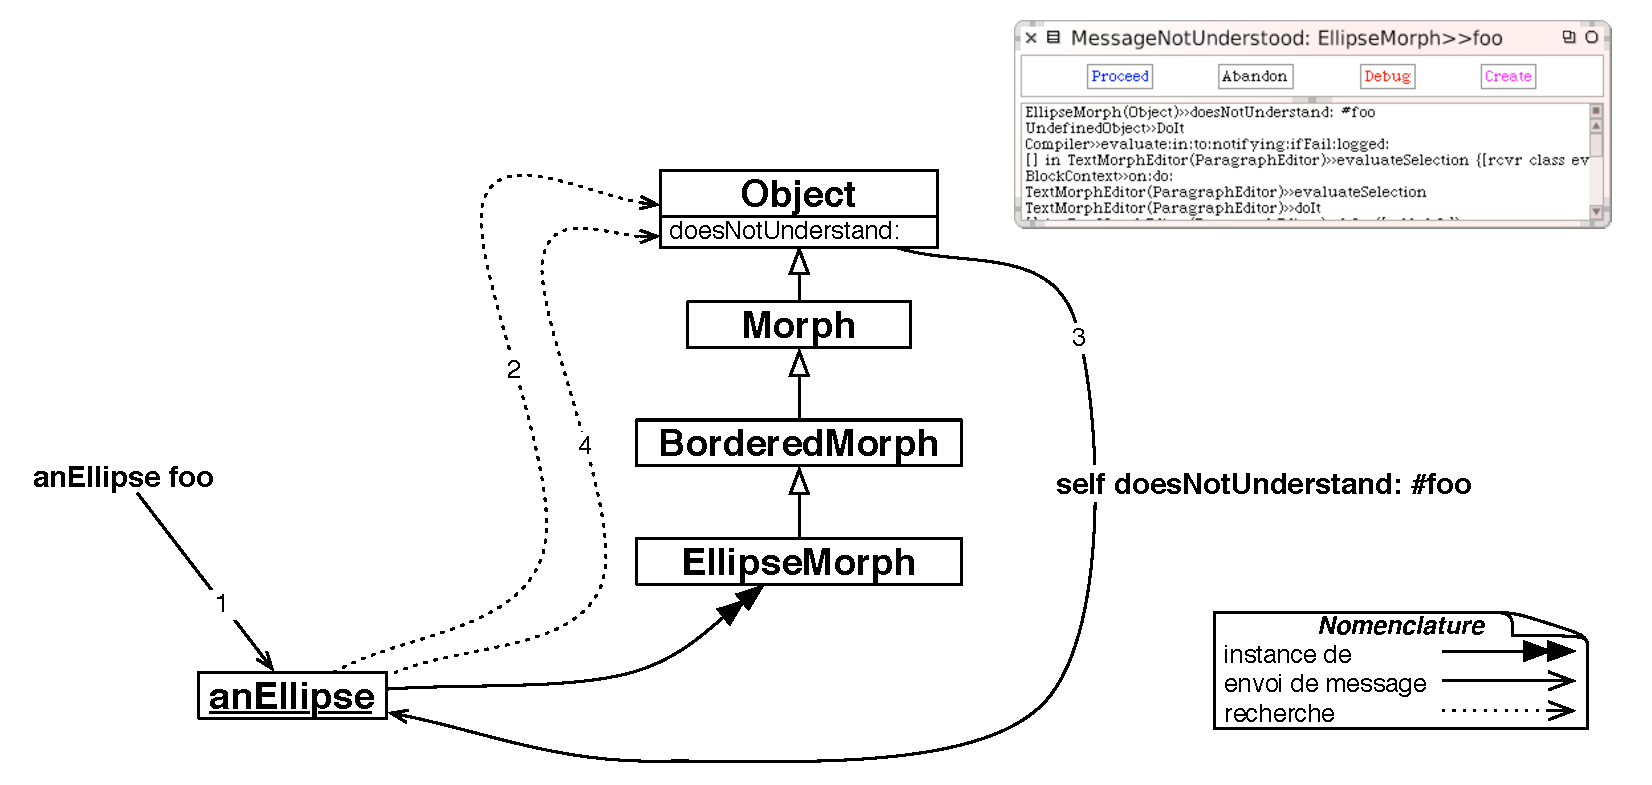
\includegraphics[width=\textwidth]{fooNotFound}}
	{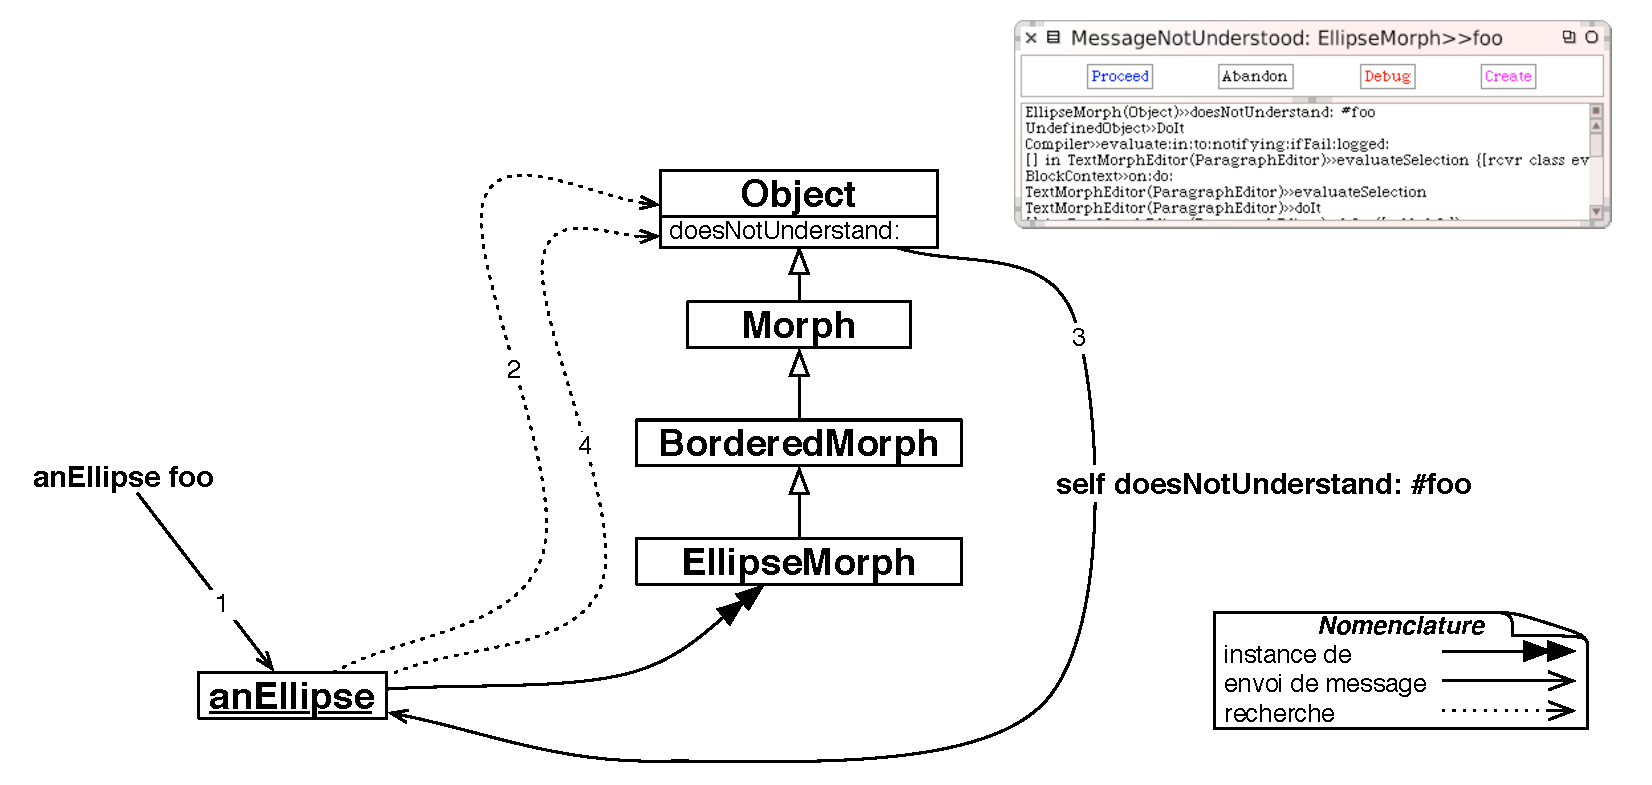
\includegraphics[width=0.8\textwidth]{fooNotFound}}
\caption{Le message \lct{foo} n'est pas compris (not understood).\label{fig:fooNotFound}}
\end{center}
\end{figure}

Ceci est un envoi dynamique de message tout \`a fait normal. Ainsi
la recherche recommence depuis la classe \ct{EllipseMorph}, mais
cette fois-ci en cherchant la m\'ethode \ct{doesNotUnderstand:}~\footnote{Le nom du message peut se traduire par: \emph{ne comprend pas}.}.
Il appara\^{\i}t que \ct{Object} impl\'emente \ct{doesNotUnderstand:}.
Cette m\'ethode cr\'eera un nouvel objet \ct{MessageNotUnderstood} (en fran\c{c}ais: Message incompr\'ehensible) capable de d\'emarrer Debugger, le d\'ebogueur, dans le contexte actuel de l'ex\'ecution.

Pourquoi prenons-nous ce chemin sinueux pour g\'erer une erreur si \'evidente?
Parce qu'en faisant ainsi, le d\'eveloppeur dispose de tous les outils pour
agir alternativement gr\^ace \`a l'interception de ces erreurs.
N'importe qui peut surcharger la m\'ethode \mthind{Object}{doesNotUnderstand:} 
dans une sous-classe de \ct{Object} en \'etendant ses possibilit\'es en
offrant une fa\c{c}on diff\'erente de capturer l'erreur.

En fait, nous nous simplifions la vie en impl\'ementant une 
d\'el\'egation automatique de messages d'un objet \`a un autre.
Un objet \ct{Delegator} peut simplement d\'el\'eguer tous les messages
qu'il ne comprend pas \`a un autre objet responsable de les g\'erer ou
de lever une erreur lui-m\^eme!

%=========================================================
\section{Les variables partag\'ees}

Maintenant, int\'eressons-nous \`a un aspect de \st que nous n'avons pas couvert
par nos cinq r\`egles: les variables \subind{variable}{partag\'ee}{}s.

\st offre trois sortes de variables partag\'ees: (1) les variables \emph{globales}; (2) les \emph{variables de classe} partag\'ees entre les instances et les classes, et (3) les variables partag\'ees parmi un groupe de classes ou \emph{variables de pool}.  Les noms de toutes ces variables partag\'ees commencent par une lettre capitale (majuscule), pour nous informer qu'elles sont partag\'ees entre plusieurs objets.
\index{variable!globale}
\index{classe!variable}
\index{variable!pool}

%---------------------------------------------------------
\subsection{Les variables globales}
En \squeak, toutes les variables globales sont stock\'ees dans un espace de nommage appel\'e \glbind{Smalltalk} qui est une instance de la classe \clsind{SystemDictionary}.
Les variables globales sont accessibles de partout.
Toute classe est nomm\'ee par une variable globale; en plus, quelques variables globales sont utilis\'ees pour nommer des objets sp\'eciaux ou couramment utilis\'es.  

La variable \glbind{Transcript} nomme une instance de \clsind{TranscriptStream}, un flux de donn\'ees ou \emph{stream} qui \'ecrit dans une fen\^etre 
\`a ascenseur (dite aussi \emph{scrollable}).
Le code suivant affiche des informations dans le \ct{Transcript} en passant une ligne.

\begin{code}{}
Transcript show: 'Squeak est extra' ; cr
\end{code}

\noindent
Avant vous lanciez la commande \menu{do it}, ouvrez un transcript en faisant un glisser-d\'eposer (drag) d'une fen\^etre Transcript depuis l'onglet (flap) \emph{Tools}~\footnote{Outils en fran\c{c}ais.}.

\hint{\'Ecrire dans le Transcript est lent, surtout quand la fen\^etre Transcript est ouverte. 
Ainsi, si vous constatez un manque de r\'eactivit\'e de votre syst\`eme alors que vous \^etes en train d'\'ecrire dans le Transcript, pensez \`a le minimiser (bouton \emph{collapse this window}).}

\subsubsection{D'autres variables globales utiles}

\begin{itemize}
\item
\ct{Smalltalk} est une instance de \ct{SystemDictionary} (Dictionnaire Syst\`eme) d\'efinissant toutes les variables globales\,---\,dont l'objet \ct{Smalltalk} lui-m\^eme.   
Les cl\'es de ce dictionnaire sont des symboles nommant les objets globaux dans le code \st.
Ainsi par exemple,
\begin{code}{@TEST}
Smalltalk at: #Boolean --> Boolean
\end{code}
Puisque \ct{Smalltalk} est aussi une variable globale lui-m\^eme,
\begin{code}{}
Smalltalk at: #Smalltalk-->a SystemDictionary(lots of globals)}
\end{code} 
et
\begin{code}{@TEST}
(Smalltalk at: #Smalltalk) == Smalltalk --> true
\end{code}

\item \clsind{Sensor} est une instance of \clsind{EventSensor}. Il repr\'esente les entr\'ees interactives ou intefaces de saisie (en anglais, \emph{input}) dans \squeak.
Par exemple, \lct{Sensor keyboard} retourne le caract\`ere suivant saisi au clavier, et \ct{Sensor leftShiftDown} r\'epond \ct{true} (vrai en bool\'een) si la
touche \emph{shift} gauche est maintenue enfonc\'ee, alors que \ct{Sensor mousePoint} renvoie un \ct{Point} indiquant la position actuelle de la souris.

\item \glbind{World} (Monde en anglais) est une instance de \clsind{PasteUpMorph} repr\'esentant l'\'ecran.
\ct{World bounds} retourne un rectangle d\'efinissant l'espace tout entier de l'\'ecran; tous les morphs (objet Morph) sur l'\'ecran sont des sous-morphs ou \emph{submorphs} de \ct{World}.
\index{Morphic}

\item \glbind{ActiveHand} est l'instance courante de \clsind{HandMorph}, la repr\'esentation graphique du curseur. Les sous-morphs de \ct{ActiveHand} tiennent tout ce qui est gliss\'e par la souris.
\ab{I have never used this, and had to browse the image to see what it is!  What do you use it for?}

\item
\glbind{Undeclared}~\footnote{Non d\'eclar\'e, en fran\c{c}ais.} est un autre dictionnaire\,---\,il contient toutes les variables non d\'eclar\'ees.
Si vous \'ecrivez une m\'ethode qui r\'ef\'erence une variable non d\'eclar\'ee,
le navigateur de classe (Browser) vous l'annoncera normalement
pour que vous la d\'eclariez, par exemple, en tant que variable globale ou variable d'instance de la classe.
Cependant, si par la suite, vous effacez la d\'eclaration, le code
r\'ef\'erencera une variable non d\'eclar\'ee. 
Inspecter \ct{Undeclared} peut parfois expliquer des comportements bizarres!

\item
\glbind{SystemOrganization} est une instance de \clsind{SystemOrganizer}: il enregistre l'organisation des classes en paquets.  Plus pr\'ecisement, il cat\'egorise les \emph{noms} des classes, ainsi
\begin{code}{@TEST}
SystemOrganization categoryOfElement: #Magnitude --> #'Kernel-Numbers'
\end{code}

\end{itemize}

Une pratique courante est de limiter fortement l'usage des variables globales;
il est toujours pr\'ef\'erable d'utiliser des variables d'instance de classe ou des variables de classes et de fournir des m\'ethodes de classe pour y acc\'eder.
En effet, si aujourd'hui \sq devait \^etre reprogramm\'e \`a partir de
z\'ero~\footnote{Le terme anglais est: \emph{from scratch}, signifiant depuis le d\'ebut.}, la plupart des variables globales qui ne sont pas des classes seraient remplac\'ees par des Singletons.

La technique habituellement employ\'ee pour d\'efinir une variable globale
est simplement de faire un \menu{do it} sur une affectation d'un identifiant
non d\'eclar\'e commen\c{c}ant par une majuscule. D\`es lors,
l'analyseur syntaxique ou \emph{parser} vous 
la d\'eclarera en tant que variable globale.  
Si vous voulez en d\'efinir une de mani\`ere programmatique, ex\'ecutez
\ct{Smalltalk at: #AGlobalName put: nil}.
Pour l'effacer, ex\'ecutez \ct{Smalltalk removeKey: #AGlobalName}.
\glbindex{Smalltalk}

%---------------------------------------------------------
\subsection{Les variables de classe}
\label{sec:classVars}

Nous avons besoin parfois de partager des donn\'ees entre les instances d'une classe et la classe elle-m\^eme.
C'est possible gr\^ace aux \emph{variables de classe}. 
Le terme \subind{classe}{variable} de classe indique que le cycle de vie
de la variable est le m\^eme que celui de la classe. Cependant, 
le terme ne v\'ehicule pas l'id\'ee que ces variables sont partag\'ees aussi bien parmi toutes
les instances d'une classe que dans la classe elle-m\^eme comme nous pouvons le voir sur \figref{privateSharedVar}.
En fait, \emph{variables partag\'ees} (ou \emph{shared variables}, en anglais) aurait
\'et\'e un meilleur nom car ce dernier exprime plus clairement leur r\^ole
tout en pointant le danger de les utiliser, en particulier si elles sont 
sujettes aux modifications.

\begin{figure}[htb]
\begin{center}
\ifluluelse
	{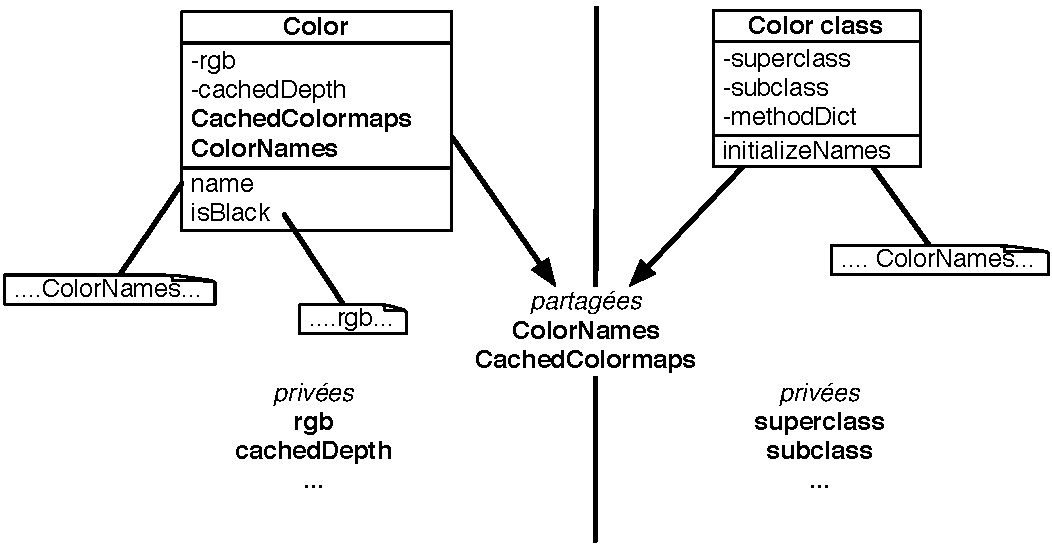
\includegraphics[width=\textwidth]{privateSharedVarColor}}
	{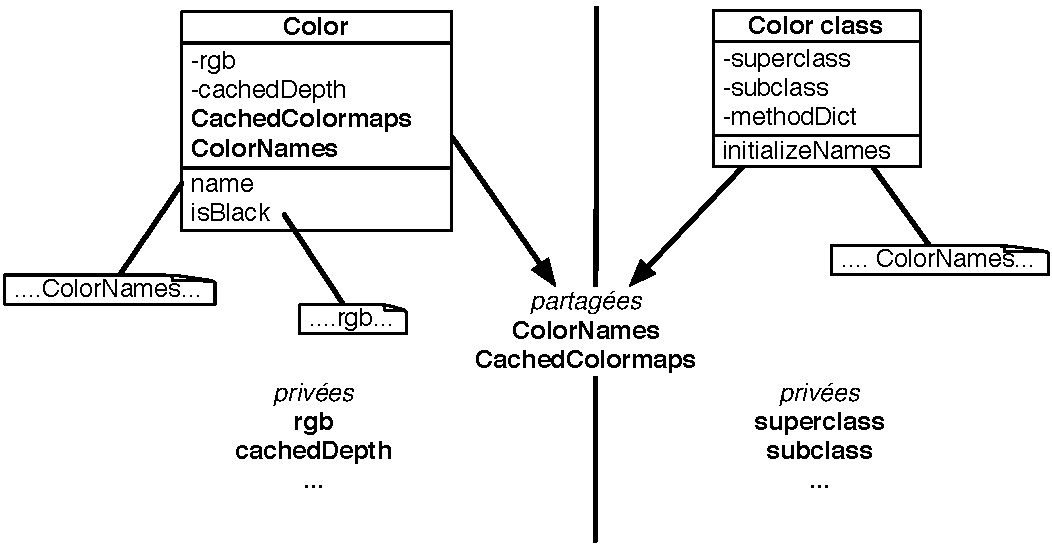
\includegraphics[width=0.7\textwidth]{privateSharedVarColor}}
\caption{Des m\'ethodes d'instance et de classe acc\'edant \`a diff\'erentes
variables.\label{fig:privateSharedVar}}
\end{center}
\end{figure}

Sur \figref{privateSharedVar} nous voyons que \ct{rgb} et \ct{cachedDepth} sont
des variables d'instance de \ct{Color} uniquement accessibles par les 
instances de \clsind{Color}.
Nous remarquons aussi que \lct{superclass}, \lct{subclass}, \lct{methodDict}\ldots \etc, sont des variables d'instance de classe, \ie des variables d'instance  accessibles seulement par \lct{Color} class.

Mais nous pouvons noter quelque chose de nouveau: \ct{ColorNames} et \ct{CachedColormaps} sont des \emph{variables de classe} d\'efinies pour \ct{Color}.
La capitalisation du nom de ces variables nous donne un indice sur le fait qu'elles sont partag\'ees.
En fait, non seulement toutes les instances de \ct{Color} peuvent acc\'eder
\`a ces variables partag\'ees, mais aussi la classe \ct{Color} elle-m\^eme, ainsi que \emph{toutes ses sous-classes}.
Les m\'ethodes d'instance et de classe peuvent acc\'eder tous les deux
\`a ces variables partag\'ees.

%\begin{figure}
%\begin{center}\includegraphics[width=6cm]{dateToday}\caption{A date is an object that  represents only anumber of days; all the information about month names, day names, etc.\ is shared among all the instances \label{fig:dateToday}}\end{center}.
%\end{figure}

Une \subind{classe}{variable} de classe est d\'eclar\'ee dans le patron
de d\'efinition de la classe.
Par exemple, la classe \ct{Color} d\'efinit un grand nombre de variables
de classe pour acc\'el\'erer la cr\'eation des couleurs;
sa d\'efinition est visible ci-dessous (\clsref{Color}).

\begin{classdef}[Color]{Color et ces variables de classe}
Object subclass: #Color 	
        instanceVariableNames: 'rgb cachedDepth cachedBitPattern'
        classVariableNames: 'Black Blue BlueShift Brown CachedColormaps ColorChart ColorNames ComponentMask ComponentMax Cyan DarkGray Gray GrayToIndexMap Green GreenShift HalfComponentMask HighLightBitmaps IndexedColors LightBlue LightBrown LightCyan LightGray LightGreen LightMagenta LightOrange LightRed LightYellow Magenta MaskingMap Orange PaleBlue PaleBuff PaleGreen PaleMagenta PaleOrange PalePeach PaleRed PaleTan PaleYellow PureBlue PureCyan PureGreen PureMagenta PureRed PureYellow RandomStream Red RedShift TranslucentPatterns Transparent VeryDarkGray VeryLightGray VeryPaleRed VeryVeryDarkGray VeryVeryLightGray White Yellow'
        poolDictionaries: '' 	
        category: 'Graphics-Primitives'
\end{classdef}

La variable de classe \cvind{ColorNames} est un tableau contenant le nom des
couleurs fr\'equemment utilis\'ees. Ce tableau est partag\'e par toutes les instances de \ct{Color} et de sa sous-classe \clsind{TranslucentColor}. 
Elles sont accessibles via les m\'ethodes d'instance et de classe.

% (see \figref{ClassVarAccess2}).

\ct{ColorNames} est initialis\'ee une fois dans \cmind{Color class}{initializeNames}, mais elle est en libre acc\`es depuis les instances de \ct{Color}.
La m\'ethode \cmind{Color}{name} utilise la variable pour trouver
le nom de la couleur.
Il semble en effet inopportun d'ajouter une variable d'instance \ct{name}
\`a chaque couleur car la plupart des couleurs n'ont pas de noms.
 
\subsubsection{L'initialisation de classe}

La pr\'esence de variables de classe l\`eve une question: comment les initialiser?

Une solution est l'\subind{classe}{initialisation} dite paresseuse (ou \emph{lazy initialization} en anglais).
Cela est possible avec l'introduction d'un message d'acc\`es qui
initialise la variable, durant l'ex\'ecution, si celle-ci n'a pas \'et\'e
encore initialis\'ee.
Ceci nous oblige \`a utiliser la m\'ethode d'acc\`es tout le temps et de ne jamais
faire appel \`a la variable de classe directement.
De plus, notons que le co\^ut de l'envoi d'un accesseur et le test d'initialisation sont \`a prendre en compte.
Ceci va \`a l'encontre de notre motivation \`a utiliser une variable de classe, parce qu'en r\'ealit\'e elle n'est plus partag\'ee.

\begin{method}[colorclasscolornames]{Color class>>colorNames}
Color class>>>colorNames	
	ColorNames ifNil: [self initializeNames].
	^ ColorNames
\end{method}	
\cmindex{Color class}{colorNames}

Une autre solution consiste \`a surcharger la m\'ethode \ct{initialize}.

\needlines{3}
\begin{method}[colorclassinit]{Color class>>initialize}
Color class>>>initialize	
	!\ldots!
	self initializeNames
\end{method}
\cmindex{Color class}{initialize}

\noindent
Si vous adoptez cette solution, vous devez vous rappeler qu'il faut
invoquer la m\'ethode \ct{initialize} apr\`es que vous l'ayez d\'efinie,
\eg en utilisant \ct{Color initialize}.
Bien que les m\'ethodes \subind{System Browser}{c\^ot\'e classe} \ct{initialize} soient ex\'ecut\'ees automatiquement lorsque le code est charg\'e en m\'emoire,
elles ne sont \emph{pas} ex\'ecut\'ees durant leur saisie et leur compilation dans le navigateur Browser ou en phase d'\'edition et de recompilation.

%---------------------------------------------------------
\subsection{Les variables de pool}
Les variables de \emph{pool}~\footnote{Pool signifie piscine en anglais, ces variables sont dans un m\^eme bain!} sont des variables qui sont partag\'ees entre plusieurs classes qui ne sont pas li\'ees par une arborescence d'h\'eritage.
\`A la base, les variables de pool sont stock\'ees dans des dictionnaires
de pool;  maintenant elles devraient \^etre d\'efinies comme variables
de classe dans des classes d\'edi\'ees (sous-classes de SharedPool).
Notre conseil: \'evitez-les. Vous n'en aurez besoin qu'en des circonstances
exceptionnelles et sp\'ecifiques.
Ici, notre but est de vous expliquer suffisamment les variables de
\subind{variable}{pool} pour comprendre leur fonction quand vous les
rencontrez durant la lecture de code.

Une classe qui acc\'ede \`a une variable de pool doit mentionner le \emph{pool}
dans sa d\'efinition de classe.
Par exemple, la classe \clsind{Text} indique qu'elle emploie le dictionnaire
de pool \ct{TextConstants} qui contient toutes les constantes textuelles
telles que 
\glbind{CR} and \glbind{LF}. 
Ce dictionnaire a une cl\'e \ct{#CR} \`a laquelle est affect\'ee la valeur
\ct{Character cr}, \ie le caract\`ere retour-chariot ou \emph{carriage return}.
\cmindex{Character class}{cr}

\begin{classdef}[textpooldict]{Dictionnaire de pool dans la classe \ct{Text}}
ArrayedCollection subclass: #Text
        instanceVariableNames: 'string runs' 	
        classVariableNames: '' 	
        !\emcode{poolDictionaries: 'TextConstants'}!
        category: 'Collections-Text'
\end{classdef}
   
Ceci permet aux m\'ethodes de la classe \ct{Text} d'acc\'eder aux cl\'es
du dictionnaire \emph{directement} dans le corps de la m\'ethode, \ie 
en utilisant la syntaxe de variable plut\^ot qu'une recherche explicite
dans le dictionnaire.
Par exemple, nous pouvons \'ecrire la m\'ethode suivante.
  
\begin{method}[texttestcr]{Text>>testCR}
Text>>>testCR 	
      ^ CR == Character cr
\end{method}

Encore une fois, nous recommandons d'\'eviter d'utiliser
les variables et les dictionnaires de pool.

%=========================================================
\section{R\'esum\'e du chapitre}

Le mod\`ele objet de \squeak est \`a la fois simple et uniforme.
Tout est un objet, et quasiment tout se passe via l'envoi de messages.

\begin{itemize}
  \item Tout est un objet.
  Les entit\'es primitives telles que les entiers sont des objets, tout comme
il est vrai que les classes soient des objets de premier ordre.

  \item Tout objet est instance d'une classe.
Les classes d\'efinissent la structure de leurs instances via des
variables d'instance \emph{priv\'ees} et leur comportement 
via des m\'ethodes \emph{publiques}. Chaque classe est l'unique
instance de sa m\'eta-classe.
Les variables de classe sont des variables priv\'ees partag\'ees par la classe
et toutes les instances de la classe.
Les classes ne peuvent pas acc\'eder directement aux variables d'instance de
leurs instances et les instances ne peuvent pas acc\'eder aux variables de
classe de leur classe.
Les m\'ethodes d'acc\`es (accesseurs et mutateurs) doivent \^etre
d\'efinies au besoin.  

  \item Toute classe a une super-classe.
  La racine de la hi\'erarchie bas\'ee sur l'h\'eritage simple est \lct{ProtoObject}.
	Cependant les classes que vous d\'efinissez devrait normalement h\'eriter de la classe \ct{Object} ou de ses sous-classes.
Il n'y a pas d'\'el\'ement s\'emantique pour la d\'efinition de classes abstraites.
Une classe abstraite est simplement une classe avec au moins une m\'ethode abstraite
\,---\,une dont l'impl\'ementation contient l'expression 
\ct{self subclassResponsibility}.
  Bien que \squeak ne dispose que du principe d'h\'eritage simple, 
il est facile de partager les impl\'ementations de m\'ethodes
en regroupant ces derni\`eres en \emph{traits}.

  \item Tout se passe par envoi de messages.
	Nous ne faisons pas des ``appels de m\'ethodes'', nous
	faisons des ``envois de messages''.
Le receveur choisit alors sa propre m\'ethode pour r\'epondre au message.

  \item La recherche de m\'ethode suit la cha\^{\i}ne d'h\'eritage;
  Les transmissions sur \self sont dynamiques et la recherche de m\'ethode
d\'emarre dans le receveur de la classe, alors que
celles sur \super sont statiques
et la recherche commence dans la super-classe de la classe dans laquelle l'envoi
sur \super est \'ecrit.

  \item Il y a trois sortes de variables partag\'ees.
Les variables globales sont accessibles partout dans le syst\`eme.
Les variables de classe sont partag\'ees entre une classe, ses sous-classes et
ses instances.
Les variables de pool sont partag\'ees dans un ensemble de classes particulier.
Vous devez \'eviter l'emploi de variables partag\'ees autant que possible.

\end{itemize}

%=========================================================
\ifx\wholebook\relax\else
   \bibliographystyle{jurabib}
   \nobibliography{scg}
   \end{document}
\fi
%=========================================================

%=================================================================
%%% Local Variables:
%%% coding: utf-8
%%% mode: latex
%%% TeX-master: t
%%% TeX-PDF-mode: t
%%% ispell-local-dictionary: "english"
%%% End:

%---------------------------------------------------------
